\documentclass[12pt, a4paper]{report}
\special{papersize=210mm, 297mm}
\usepackage[english]{babel}
\usepackage[utf8x]{inputenc}
\usepackage[left=2.5cm, right=2.5cm, top=2.5cm]{geometry}
\renewcommand{\baselinestretch}{1.4}
\usepackage[toc,page]{appendix}
\pagenumbering{alph}

\usepackage{amsmath}
\usepackage{graphicx}
\usepackage{float}
\graphicspath{{images/} {diagrams/}}
\usepackage{tabularx}
\usepackage{booktabs}
\usepackage[linesnumbered,ruled]{algorithm2e}

%\usepackage{showframe}
\usepackage{fullpage}

\usepackage{url}
%\usepackage{natbib} % for author-date citation \citep{}, \citet[]
%\usepackage{hyperref}
%\usepackage[nottoc]{tocbibind}
\usepackage{listings}
\usepackage{verbatim}
\usepackage{color}

\definecolor{dkgreen}{rgb}{0,0.6,0}
\definecolor{gray}{rgb}{0.5,0.5,0.5}
\definecolor{mauve}{rgb}{0.58,0,0.82}

\lstset{frame=tb,
	language=java,
	aboveskip=5mm, belowskip=3mm, showstringspaces=false,
	columns=flexible, basicstyle={\small\ttfamily},
	numbers=none, numberstyle=\tiny\color{gray},
	keywordstyle=\color{blue},
	commentstyle=\color{dkgreen},
	stringstyle=\color{mauve},
	breaklines=true,
	breakatwhitespace=true,
	tabsize=3
}


\usepackage{multirow}
\usepackage{array}
\newcolumntype{L}[1]{> {\raggedright\let\newline\\\arraybackslash\hspace{0pt}}m{#1}}
\newcolumntype{C}[1]{>{\centering\let\newline\\\arraybackslash\hspace{0pt}}m{#1}}
\newcolumntype{R}[1]{>{\raggedleft\let\newline\\\arraybackslash\hspace{0pt}}m{#1}}

\pagenumbering{arabic}

\begin{document}
	
	%======================================================================
	
	\begin{titlepage}
		
		\newcommand{\HRule}{\rule{\linewidth}{0.5mm}}
		
		\center
		
		\vspace{-20pt}
		
\includegraphics[width=100pt]{../images/FMI-03.png}\\[1.0cm]
		
		\textsc{\LARGE West University of Timisoara}\\[0.5cm]
		\textsc{\Large Faculty of Mathematics and Computer Science}\\[0.5cm]
		\textsc{\large Study Program: \\Computer Science in English}\\[3cm]
		\textsc{\Huge Master Dissertation}\\[5cm]
		
		\begin{minipage}{0.4\textwidth}
			\begin{flushleft} \large
				\textbf{COORDINATOR:}\\
				Associate Prof. Marc Eduard \textsc{Frîncu}
			\end{flushleft}
		\end{minipage}
		~
		\begin{minipage}{0.4\textwidth}
			\begin{flushright} \large
				\textbf{GRADUATE:} \\
				Maria Minerva \textsc{Vonica}
			\end{flushright}
		\end{minipage}\\[0.5cm]
			
		\vfill
		{\large Timi\c{s}oara \\2021}\\
		\vfill
		
	\end{titlepage}
	
	% =====================================================================
	
	\begin{titlepage}
		
		\newcommand{\HRule}{\rule{\linewidth}{0.5mm}}
		
		\center
		
		\textsc{}\\[.7cm]
		
		\textsc{\LARGE West University of  Timi\c{s}oara}\\[0.5cm]
		\textsc{\Large Faculty of Mathematics and Computer Science}\\[0.5cm]
		\textsc{\large Study Program: \\Computer Science in English}\\[4.5cm]
		
		\textsc{\Huge Master Dissertation}\\[2cm]
		
		{\Huge \bfseries Name}\\[6cm]
		
		\begin{minipage}{0.4\textwidth}
			\begin{flushleft} \large
				\textbf{COORDINATOR:}\\
				Associate Prof. Marc Eduard \textsc{Frîncu}
			\end{flushleft}
		\end{minipage}
		~
		\begin{minipage}{0.4\textwidth}
			\begin{flushright} \large
				\textbf{GRADUATE:} \\
				Maria-Minerva \textsc{Vonica}
			\end{flushright}
		\end{minipage}\\[0.5cm]
		\vfill
		{\large Timi\c{s}oara\\ 2021}\\
		
		\vfill
		
	\end{titlepage}

	% =====================================================================
	
	\begin{abstract} %begin abstract  
		%The abstract should have one page and should be a compact presentation of the dissertation.
		\vspace{1.0cm}
		\vspace{1.0cm}
		\par
		
		Over the last decade, climate change has impacted Earths' atmosphere and environment more than anytime before. Studies held by NASA confirmed that the second hottest year ever recorded was 2019 and the recorded temperatures of the ocean have never been higher. One way to track these changes is to study the retreat of glaciers, since they are the most sensitive climate change indicators. Since NASA and USGS launched their first Earth observation satellite in 23 July 1972, millions of images of the Earth have been stored and are freely to use for various fields of research. 
		\vskip 0.2cm
		Having this in mind, the goal of our application is to analyse the retreat of glaciers over time by using advanced computer vision algorithms which are able to detect movement of pixels based on a time series of aerial scenes collected from the Landsat 8 satellite. By analysing the directions of glacier retreat over time, we try to generate future images of how they might change. The snowfall and ice percentages of a glacier for a satellite image are also taken into consideration as a validation of our results. The application has also been made with the goal of being simple to use and easy to access for anyone who wants to get involved and make a contribution. 
		\vskip 0.2cm
		This thesis contains information about the application's functionality, processing mechanics and experiments on various glaciers. In order to have a self sufficient environment,  both search and download of Landsat 8 assets facilities have been made available, such that one does not need to have an already created dataset of glacier satellite images.  As for generating a motion predicted image, we need to extract movement information between two consecutive snow index scenes which produces vectors of movement for each pixel. These results are used to further extend this movement trend which generates a predicted image.
		
	\end{abstract} %end abstract

	\newpage{}

	\tableofcontents{}
	\addcontentsline{toc}{chapter}{List Of Figures}
	\listoffigures{}
	\addcontentsline{toc}{chapter}{List Of Tables}
	\listoftables{}
	
	\newpage{}

	\chapter{Introduction}
	
	\par The aim of Earth observation satellites is to collect satellite imagery in a consistent and long-term manner. These images can then further be used in order to extract information on weather behaviour, ocean temperatures, vegetation health, droughts and various other environmental variables. There are application which extract patterns based on these factors in order to understand why certain phenomena happened in the past and what are the conditions required for them to reappear in the future as well. 
	
	\par However, applications which track these changes require large processing power and consistent, qualitative datasets. Most of these datasets can be freely accessed and various analysation techniques can be used in order to extract pattern changes throughout the years. Fortunately, there are numerous Earth observing satellites which could satisfy the requirements of such a dataset. For the purpose of this thesis, only images collected by the Landsat 8 satellite have been used, since their quality is better than the last missions.
	
	\section{Motivation and goals}
	
	\par The motivation behind this thesis is found in the background of what climate change meant in the past and what it could further inquire in the future. Carbon dioxide levels in the atmosphere grown more than they can be naturally eliminated, causing butterfly effect changes in the environment. Glaciers are the most sensitive to these changes and through the means of Erath observation satellites they have been tracked longed enough such that qualitative imagery research can be used on them. On top of this, over the last years we have developed more and more powerful tools which are able to process heavy amounts of data. Not taking advantage of these factors seems like a loss.
	
	\par The goal of this thesis is to make use of such data by creating a tool for easy dataset creation, as well as analysing changes of glaciers in the last decade with the purpose of creating predicted images which could highlight future glacier retreat and snow fall decrease.

	\section{Related work} 

	\par There are multiple research papers on the domain of glacier analysis. Some of those which we found useful for our research regarding analysis of glacier based on satellite imagery are:
	\begin{itemize}
		\item \cite{rgmuos}, which proposes various methods of mapping glaciers on satellite images while taking into consideration seasonal variations in spectral properties of snow; 
		\item \cite{aaesakh}: methods for separating ice and snow from debris using different indicators to calculate the mass balance of the glacier;
		\item \cite{parvati}: assessment of glacier mass loss through a remote sensing modelling framework;
		\item \cite{sar}: tracking transient snow lines and investigating firn evolution;
		\item \cite{msg}: methods for measuring snow and glacier ice properties with the use of new satellite sensors, such as synthetic aperture radar.
	\end{itemize}

	For the alignment part of the thesis, some of the most helpful papers were \cite{orbsift}, \cite{feorb} and \cite{orblocal} which describe different ways in which we can pair the ORB alignment algorithm with different methods of warping and feature point extraction.

	\section{Our Contribution}
	
	\par This thesis makes use of techniques such as computer vision and machine learning for generating predicted images based on detected motion. This can be used to highlight glacier retreat over longer periods of time. For this purpose we had to implement techniques to align our images with respect to a reference, as well as determining ways to make use of the extracted optical flow information such that we can generate new images.

	\par For the alignment process, more than 200 pairs of images have been tested, while only 10\% of them having erroneous alignment results. As for the image generation, the results can be seen in the Section~\ref{seq:performance}. TODO MORE TO WRITE HERE, SOME NUMBERS. Since the generated images rely mostly on visual validation, we have compared the ice and snow coverage on multiple datasets with different coordinates. TODO WRITE THIS BETTER.
	
	\par The results were achieved through indexing glacier datasets by a crawler, which later on structure the data into path and row coordinates (see Paragraph~\ref{par:wrs2}), such that we are working with geographically consistent data. The normalized snow difference index has been calculated as described in Section~\ref{seq:ndsi_functional}, by using two Landsat 8 bands. We have chosen this metric to enhance snowfall and ice due to their high reflectance in the visible spectrum and high absorption in the infrared one.
	
	\par Our goal is to process these images as pairs, so we had to take into consideration the fact that Landsat 8 does not have a perfectly stable trajectory, which yields in slightly misaligned pictures. However, this discrepancy would prove to generate unreliable results in the predicted image, therefore multiple techniques of solving this problem have been tested. Details of these can be found at Section~\ref{seq:alignment_functional}.

	\par For the image generation we used a computer vision algorithm which calculated the optical flow between two consecutive frames, which resulted in a matrix holding the distance of movement for each pixel. Based on this distance, new coordinates have been predicted for the pixels and they have been moved accordingly, resulting in a new image representing the change over time. Various methods of filtering have been applied on the results, as it is described in Section\ref{seq:motion_ndsi_functional}. In order to validate our results, we have computed predicted images for all the pairs of the dataset, and we have compared them to already existing consecutive ones. The snow and ice coverage of the motion generated image can be then compared with its neighbours.

	\par Since our application focuses on working with images, a graphical user interface seemed fit for this purpose. However, for the search and download part, a simple command line script has been used (see Section~\ref{seq:gui}.
	
	\newpage{}
	
	\chapter{Application}
	\section{Dataset}
	\par In order to build the dataset, we made use of the freely available data from the Landsat Archive, specifically from collection 1, level 1. This dataset contains assets which are generated from the Landsat 8 Sensors, as well as entries from other older Landsat satellites. For the purpose of this paper, we will focus only on images collected from the Landsat 8 satellite.
	
	\subsection{Landsat 8}
	\label{seq:landsat8_section}

	\par We will use images collected by the Landsat 8 satellite (Figure~\ref{fig:landsat_satellite}), which was the most recently lauched on the Atlas-V rocket (Vandenberg Air Force Base), in California on February 11, 2013. For remote sensing, Landsat 8 is equipped with two sensors, the Thermal Infrared Sensor (TIRS)  and Operational Land Imager (OLI) one.
	\begin{figure}[h!]
		\centering
		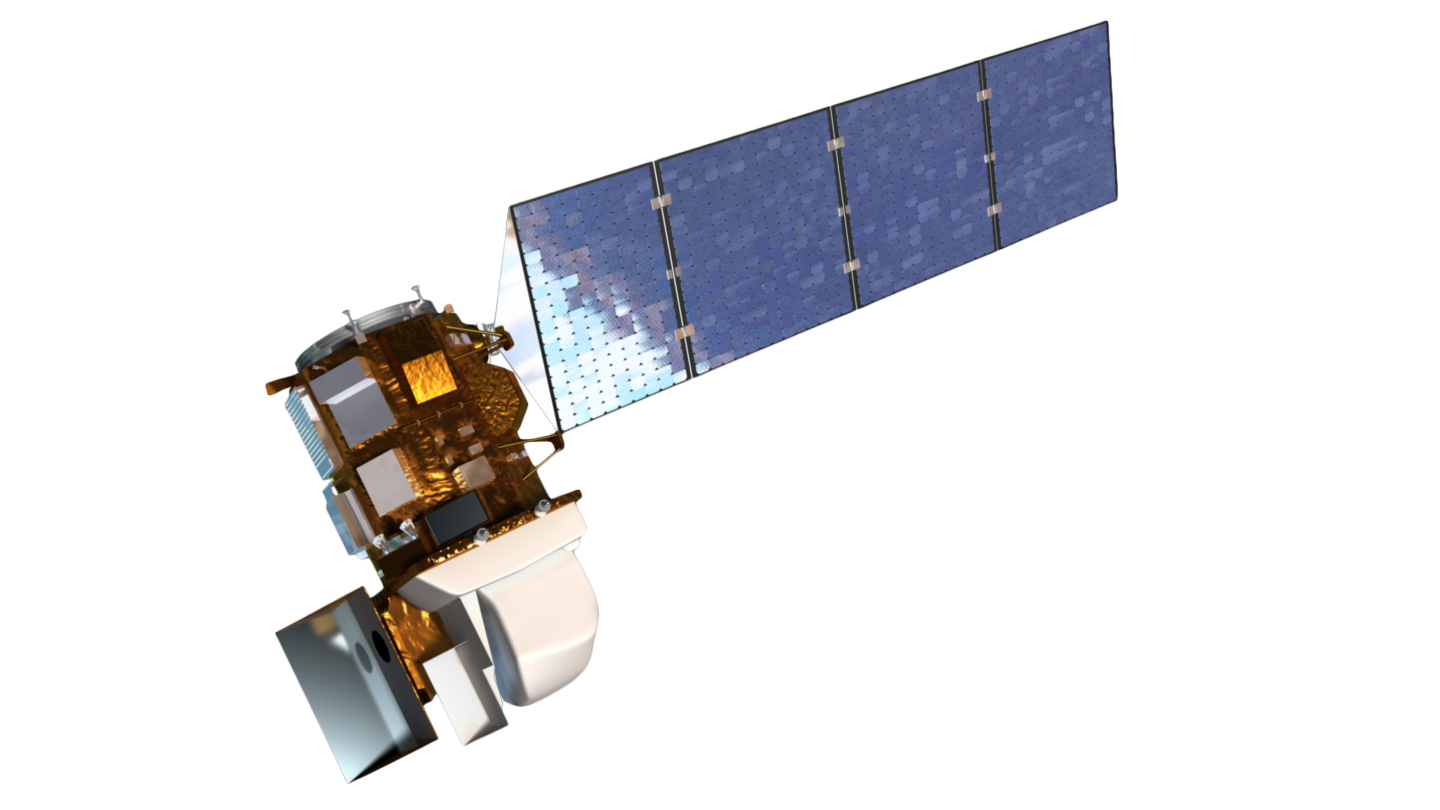
\includegraphics[scale=0.25]{../images/LandsatSatellite.png}
		\caption{Landsat 8 satellite \cite{LANDSATPIC}}
		\label{fig:landsat_satellite}
	\end{figure}

	\par The satellite is orbiting the Earth at an altitude of 705 km, completing one orbit every 99 minutes. Based on this trajectory, the satellite has a 16 day repeat cycle and it acquires 740 scenes each day. These are organised on the path/row system defined by Worldwide Reference System-2 (WRS-2). A Landsat 8 scene size is 185 km x 180 km \cite{LANDSAT}. 
	
	\paragraph{Worldwide Reference System-2}
	\label{par:wrs2}
	
	\par We will be referring to each scene's location based on its path and row coordinates from the worldwide reference system-2, which is a notation system used for Landsat images. This system is used with the main goal of keeping a structured archive of Landsat data which can be easily catalogued and accesses. Users can access aerial imagery through querying the specified path and row variables \cite{wrs}. Landsat's trajectory projected on the world map can be seen in Figure~\ref{fig:wrs2}.
	\begin{figure}[h]
		\centering
		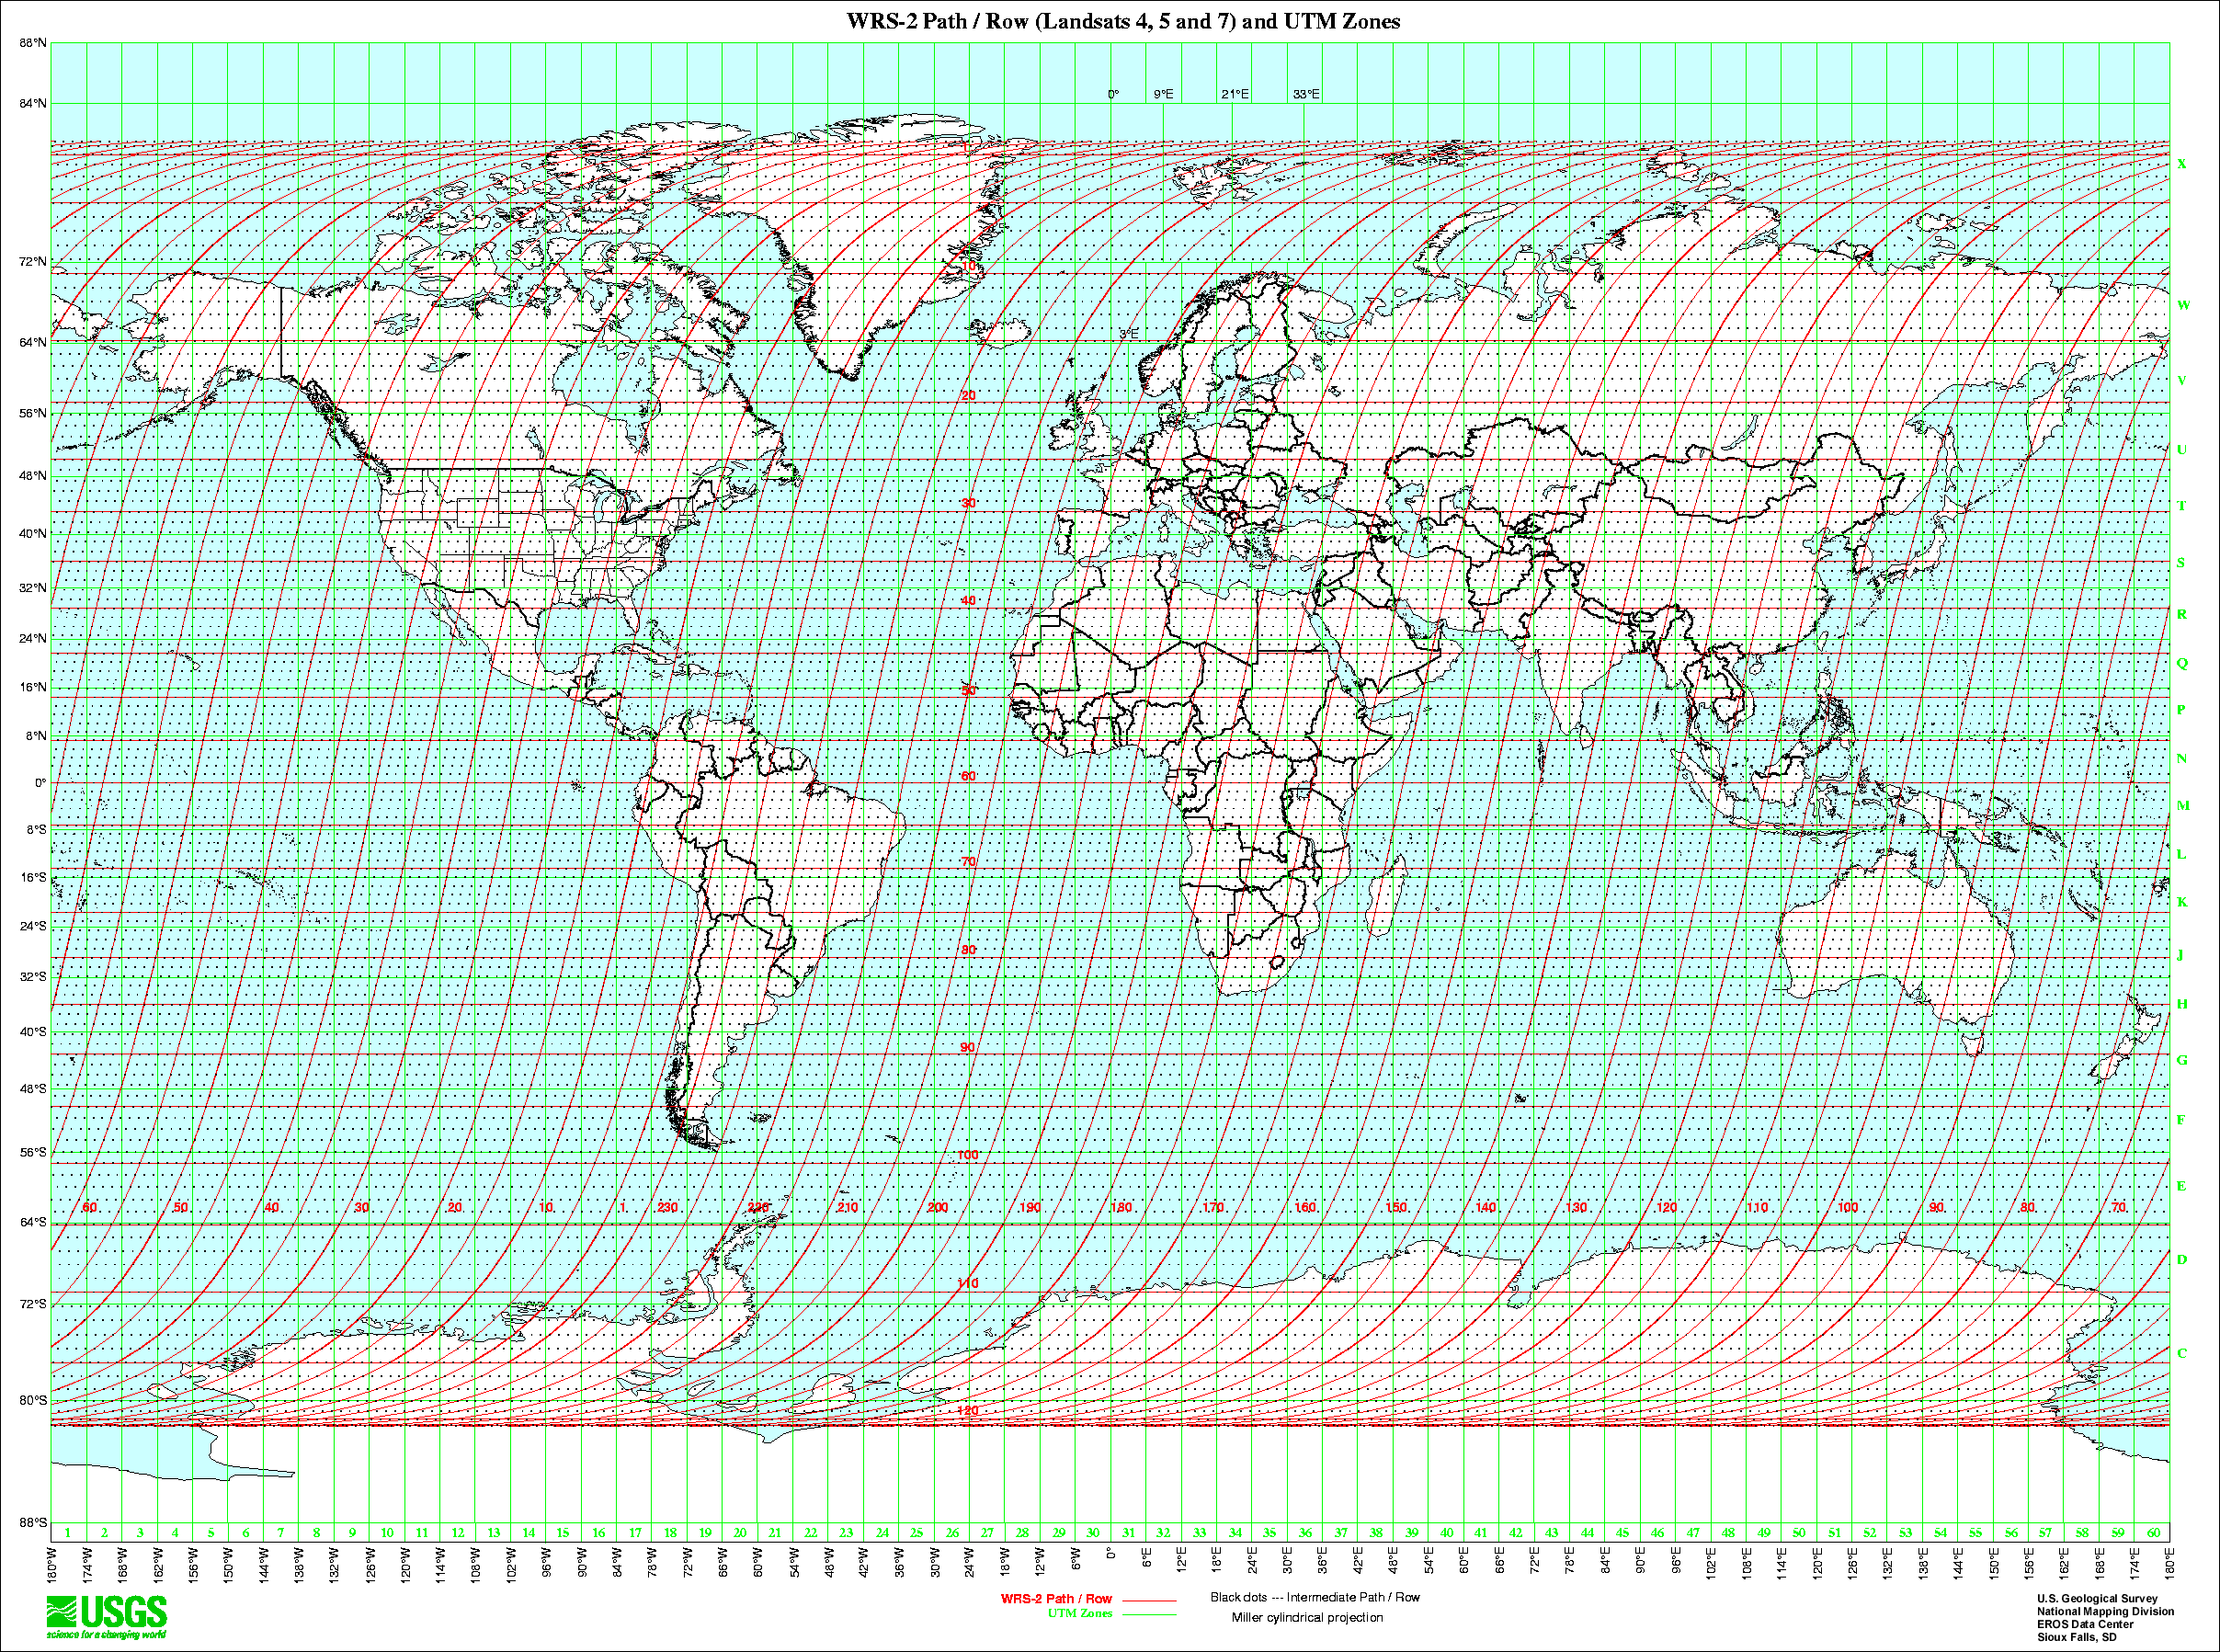
\includegraphics[scale=0.2]{../images/wrs2.png}
		\caption{WRS-2 Path/Row for Landsat \cite{wrs}.}
		\label{fig:wrs2}
	\end{figure}
	
	\subsubsection{Landsat scene naming convention}
	\label{seq:landsat_naming}
	
	\par Each Landsat scene is named after a well-defined convention in order to easily check information such as the WRS path, row and the date of acquisition. Having access to this information without the need to download the scene itself or the metadata file which holds this information represents a valuable asset, since we can easily filter the data based on the naming convention itself. In the table \ref{table:landsat_table} below we represent what each part of a Landsat scene of the form \textbf{LXS PPPRRR YYYYDDD GSIVV} means.
	\begin{table} [h]
		\center
		\begin{tabularx}{480pt}{|X|X|}
			\toprule
			\textbf{L} & Landsat \\ [0.2ex]
			\midrule
			\textbf{X} & Sensor \\ [0.2ex]
			\midrule
			\textbf{SS} & Satellite \\ [0.2ex]
			\midrule
			\textbf{PPP} & WRS path \\ [0.2ex]
			\midrule
			\textbf{RRR} & WRS row \\ [0.2ex]
			\midrule
			\textbf{YYYY} & Acquisition year \\ [0.2ex]
			\midrule
			\textbf{DDD} & Julian day of the acquisition year \\ [0.2ex]
			\midrule
			\textbf{GSI} & Ground station identifier \\ [0.2ex]
			\midrule
			\textbf{VV} & Archive version number \\ [0.2ex]
			\midrule
			\midrule
			\bottomrule
		\end{tabularx}
		\caption{Landsat 8 scene naming convention \cite{sn}.}
		\label{table:landsat_table}
	\end{table}
	
	\subsubsection{Operational Land Imager}
	
	\par The Operational Land Imager (OLI) represents remote sensing instrument which can be found abroad Landsat 8. It is built by Ball Aerospace \& Technologies and it collects moderate resolution data which is used for monitoring changes in trends on the surface and evaluating how it changes over time. The images and data which OLI has helped collect have practical applications today in various fields such as mapping and monitoring changes in snow, ice, water and agriculture, \cite{lolidcp}. 
	The OLI operates in the short wave infrared spectral and visible region with a width of 185 km. Wavelengths of 443 nm to 2,200 nm are translated into nine channels, from which  eight are multispectral and one is panchromatic. The eight multispectral ones have a 30-meter spatial resolution, while the panchromatic channel has a 15 meters one.
	The OLI generates 9 bands for Landsat as shown in Figure~\ref{fig:L8OLI}.
	\begin{figure}[h]
		\centering
		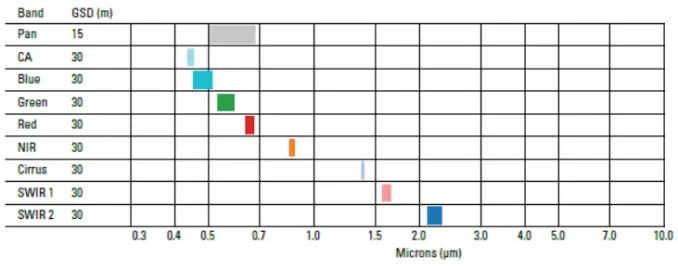
\includegraphics[scale=0.5]{../images/Landsat8-OLI-Bands.png}
		\caption{Landsat 8 OLI generated bands \cite{l8otb}}
		\label{fig:L8OLI}
	\end{figure}
	
	\subsubsection{Thermal Infrared Sensor}
	
	\par The Thermal Infrared Sensor (TIRS) measures land surface temperature in two thermal bands with a new technology that uses quantum mechanic techniques in order to detect thermal infrared wavelengths of light which are emitted by the Earth \cite{lgng}. The thermal infrared sensor generates 2 bands for Landsat as shown in Figure~\ref{fig:L8TIRS}.
	
	\begin{figure}[h!]
		\centering
		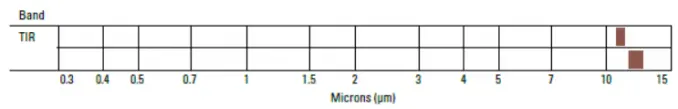
\includegraphics[scale=0.5]{../images/Landsat8-TIRS-Bands.png}
		\caption{Landsat 8 TIRS generated bands \cite{l8otb}}
		\label{fig:L8TIRS}
	\end{figure}
	
	\subsubsection{OLI and TIRS bands}
	
	Landsat 8 acquires data from these sensors in in 11 bands, as following in Table~\ref{table:bands_table}.
	
	\begin{table} [h]
		\center
		\begin{tabularx}{480pt}{|p{0.3\linewidth}|X|X|}
			\toprule
			\textbf{Bands} & \textbf{Wavelength (micrometers)} & \textbf{Resolution (meters)} \\ [0.2ex]
			\midrule
			\midrule
			Band 1 (Coastal aerosol) & 0.43-0.45 & 30 \\ [0.2ex]
			\midrule
			Band 2 (Blue) & 0.45-0.51 & 30 \\ [0.2ex]
			\midrule
			Band 3 (Green) & 0.53-0.59 & 30 \\ [0.2ex]
			\midrule
			Band 4 (Red) & 0.64-0.67 & 30 \\ [0.2ex]
			\hline
			Band 5 (Near Infrared) & 0.85-0.88 & 30 \\ [0.2ex]
			\midrule
			Band 6 (SWIR1) & 1.57-1.65 & 30 \\ [0.2ex]
			\midrule
			Band 7 (SWIR2) & 2.11-2.29 & 30 \\ [0.2ex]
			\midrule
			Band 8 (Panchromatic) & 0.50-0.68 & 15 \\ [0.2ex]
			\midrule
			Band 9 (Cirrus) & 1.36-1.38 & 30 \\ [0.2ex]
			\midrule
			Band 10 (TIR 1) & 10.6-11.19 & 100  \\ [0.2ex]
			\midrule
			Band 11 (TIR 2) & 11.50-12.51 & 100 \\ [0.2ex]
			\midrule
			\bottomrule
		\end{tabularx}
		\caption{Landsat 8-9 Operational Land Imager (OLI) and Thermal Infrared Sensor (TIRS) bands \cite{bands}.}
		\label{table:bands_table}
	\end{table}
	
	\subsection{World Glacier Inventory}
	\label{seq:wgi}
	
	\par The World Glacier Inventory (WGI) proves to be a useful resource for building our dataset, since it contains over 130,000 entries representing glaciers. Various parameters are stored in this file for each glacier, such as its geographic location in the form of latitude and longitude coordinates, total area, its elevation, orientation and many more. The dataset has been constructed through aerial satellite mapping,therefore the set can be viewed as a snapshot of the glacier distribution from 2012 \cite{WGI}.  
	
	\par There are a number of ways to retrieve data from the inventory:
	\begin{itemize}
		\item download the dataset in a single CSV file (wgi\_feb2012.csv);
		\item search by parameter using the Search Inventory interface;
		\item extract regions through the Extract Selected Regions interface.
	\end{itemize}

	\par The CSV text file will be used with the purpose to define which are the glaciers to be included in the dataset to be built. An example of how this file looks like can be found in Figure~\ref{fig:WGI_ASCII}.
	
	\begin{figure}[h]
		\centering
		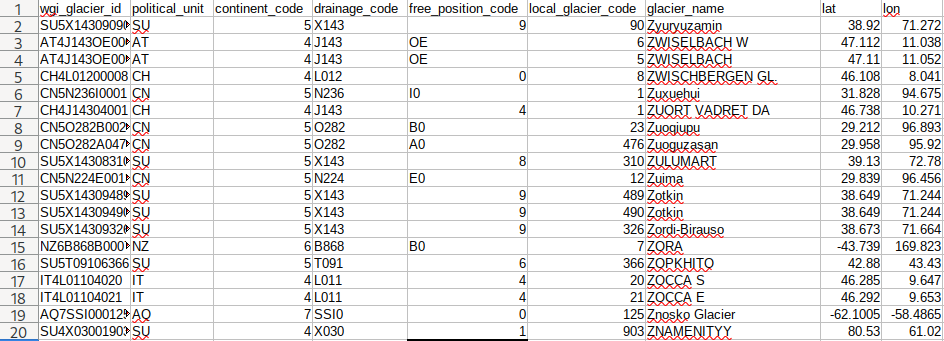
\includegraphics[scale=0.5]{../images/wgi_ASCII_file.png}
		\caption{World glacier inventory ASCII text file, as CSV}
		\label{fig:WGI_ASCII}
	\end{figure}
	
	\par The parameters which will be extracted for the dataset construction are the following:
	\begin{itemize}
		\item \textbf{wgi\_glacier\_id}: unique id representing one glacier (or part of it, if the coverage area is larger);
		\item \textbf{glacier\_name}: name of the glacier (if it has one);
		\item \textbf{lat}: latitude of the glacier;
		\item \textbf{lon}: longitude of the glacier.
	\end{itemize}

	\subsection{Asset Acquisition}
	
	\par Since Landsat 8 acquires over 700 scenes per day, this means that there are over two million scenes available for download, either making use of already built user friendly tools or by simply querying for them directly.
	
	\subsubsection{USGS Earth Explorer}
	
	\par One of the most popular services for satellite imagery downloading is USGS Earth Explorer. This is used for querying and ordering of satellite images, aerial photographs, and cartographic products through the U.S. Geological Survey. The tool is particularly useful when the main focus is to analyse a specific area rather than trying to acquire a large dataset of scenes. One can easily search for assets based on criteria such as world reference system path and row variables, latitude, longitude, cloud coverage, capture date and many others \cite{USGS}.
	
	\par However, downloading a large set of assets proves to be rather difficult by using this tool alone, since the parameters for each scene need to be manually set. On top of this, the query results have to be picked by hand and then passed for downloading through another application which handles their bulk download. This makes the process of building the dataset rather slow, frustrating and error prone. Such an example can be viewed in Figure~\ref{fig:EarthExplorer}, for the Belvedere glacier (45.942, 7.908).
	
	\begin{figure}[h]
		\centering
		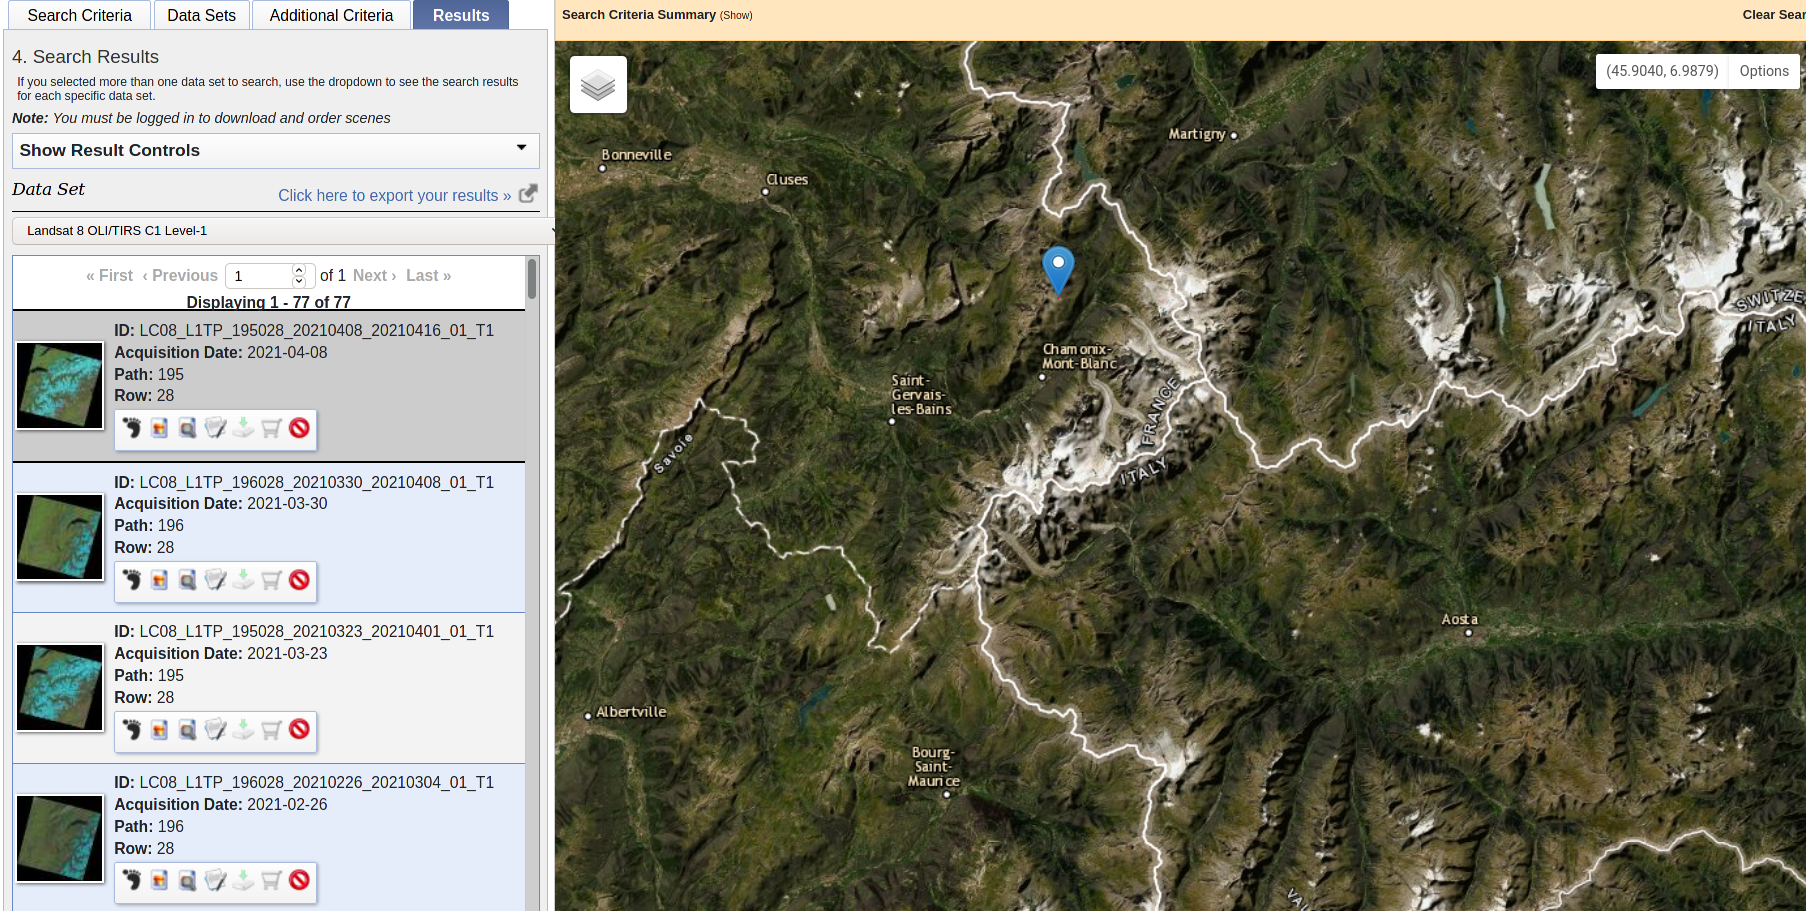
\includegraphics[scale=0.25]{../images/EarthExplorer.png}
		\caption{EarthExplorer}
		\label{fig:EarthExplorer}
	\end{figure}
	
	\subsubsection{SpatioTemporal Asset Catalog API}
	\label{seq:STAC}
	
	\par In order to fix the problem of excessive manual labour which appeared by using the USGS Earth Explorer, we rather implemented an endpoint of the SpatioTemporal Asset Catalog API, specifically, the following: \textbf{\url{http://nsidc.org/data/glacier_inventory/index.html}} \cite{STAC}. The main idea of searching by using parameters still remains, but instead of manual inputting data for the search data, we rely on using the above-mentioned World Glacier Inventory ASCII text file, since it already has all the required information for each glacier.
	
	\par By using this method we can pick which glaciers we want to download based on their coordinates and calculate a bounding box representing the area we want to search, required for the STAC API query. Since there might be clouds which could obfuscate the area of interest in the image, we also add a maximum allowed cloud coverage along the bounding box.
	
	\par The STAC API query also requires a name for the collection of assets we want our queries to be made on, which for us is landsat-8-l1 (Landsat 8 Collection 1, Level 1). Using these three parameters we can now easily acquire a large number of assets with minimal manual labour, as compared to the more user friendly tool provided by USGS.
	
	\par The downloaded assets will be stored at a user specified disk location and they will be structured as shown in the Figure~\ref{fig:DownloadDirectory}.
	\begin{figure}[h]
		\centering
		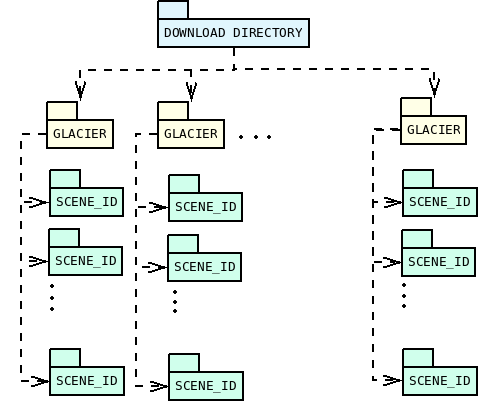
\includegraphics[scale=0.4]{../images/DownloadDirectory.png}
		\caption{Download Directory}
		\label{fig:DownloadDirectory}
	\end{figure}
	
	\subsubsection{Landsat 8 Collection 1, Tier 1}
	
	\par To support analysis  of the Landsat long-term data record, the Landsat archive was restructured into a more formal data collection structure with the aim of keeping consistent information for each level 1 product. By making sure that these standards are met, the library can be used for various applications such as data stacking and time-series analysis \cite{lc1l1}. By using data from this collection, we ensure that our images are fit for accurate pixel-to-pixel processing.
	
	\section{Dataset entities}
	
	\par We will further describe which are the bands necessary for the image generation and what are their uses. On top of this, we will further explain what is the normalized snow difference index and what is the optical flow used for.
	
	\subsection{Bands}
	
	\par Each Landsat 8 band is represented by a 16 bit grayscale image with a resolution between 7000 and 10000 pixels, each pixel representing 30 meters. We can conclude, therefore, that one scene covers around 200 and 300 km of Earth. Only the green and SWIR1 bands will be used for the purpose of this thesis and below we will discuss the specifications of each. 
	
	\subsubsection{Band 3 - Green Band}
	
	\begin{table} [h]
		\center
		\begin{tabular} {| l | l |}
			\hline
			\textbf{Wavelength} & {0.53- 0.59 micrometers} \\ [0.2ex]
			\hline
			\textbf{Spacial resolution} & {30 meters} \\ [0.2ex]
			\hline
			\textbf{Resolution} & {between 7000x7000 pixels and 10000x10000 pixels} \\ [0.2ex]
			\hline
			\textbf{Depth} & {16-bit}\\ [0.2ex]
			\hline
			\textbf{Format} & {grayscale}\\ [0.2ex]
			\hline
		\end{tabular}
		\caption{Landsat 8 green band specifications.}
		\label{table:green_table}
	\end{table}
	\par The green band, alongside with the red and blue ones, fall in the visible spectrum and it is usually used for mapping peak vegetation. Figure~\ref{fig:green} is an example of the green band for the LC81950282015098LGN01 scene.
	\begin{figure}[h]
		\centering
		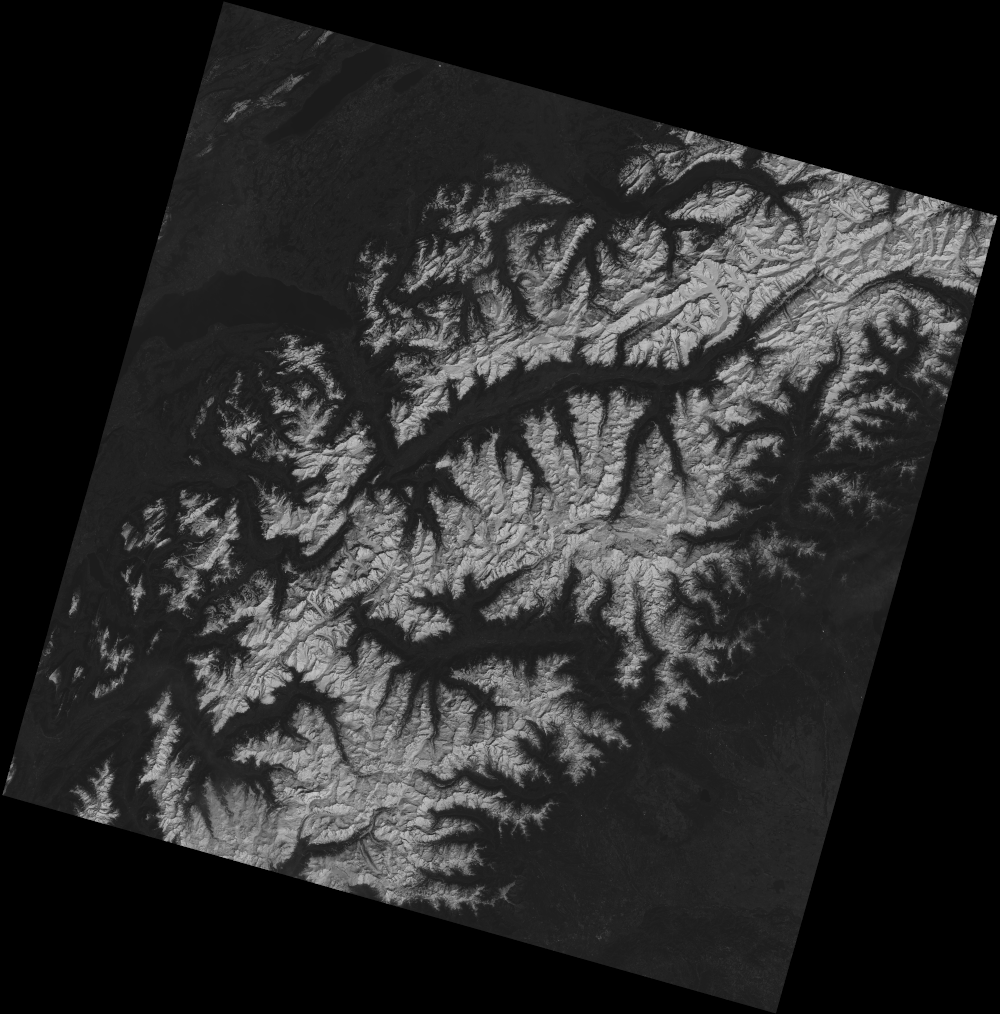
\includegraphics[scale=0.3]{../images/LC81950282015098LGN01_B3.png}
		\caption{Green band of scene LC81950282015098LGN01.}
		\label{fig:green}
	\end{figure}
	
	\subsubsection{Band 6 - SWIR1 Band}
	
	\begin{table} [h]
		\center
		\begin{tabular} {| l | l |}
			\hline
			\textbf{Wavelength} & {1.57 - 1.65 micrometers} \\ [0.2ex]
			\hline
			\textbf{Spacial resolution} & {30 meters} \\ [0.2ex]
			\hline
			\textbf{Resolution} & {between 7000x7000 pixels and 10000x10000 pixels} \\ [0.2ex]
			\hline
			\textbf{Depth} & {16-bit}\\ [0.2ex]
			\hline
			\textbf{Format} & {grayscale}\\ [0.2ex]
			\hline
		\end{tabular}
		\caption{Landsat 8 SWIR1 band specifications.}
		\label{table:swir1_table}
	\end{table}
	\par The shortwave infrared 1 band is particularly useful for enhancing object which look similar in other bands, such as soils and rocks \cite{bd}. Alongside this, it also discriminates moisture content of soil and vegetation and penetrates thin clouds \cite{bands}. Figure~\ref{fig:swir1} is illustrated below as an example of a SWIR1 band taken from the same scene as the green one above.
	\begin{figure}[h]
		\centering
		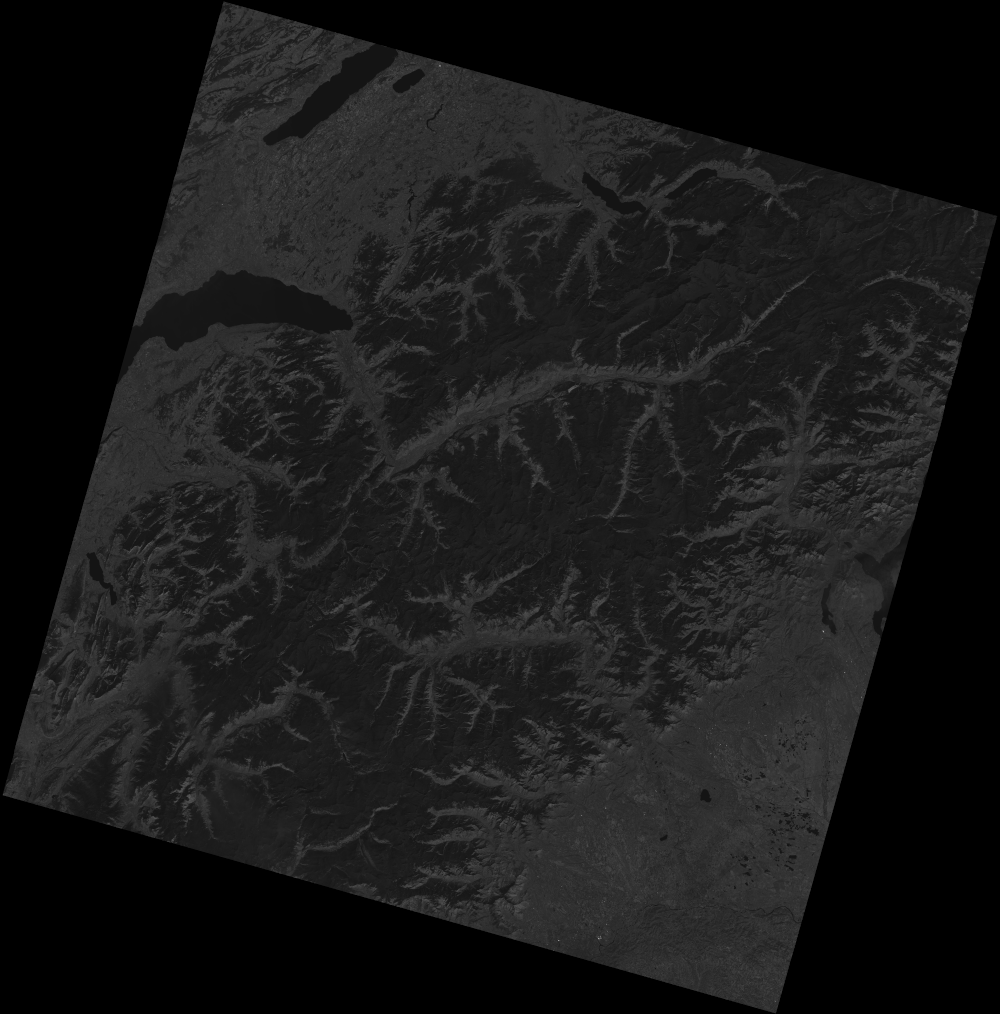
\includegraphics[scale=0.3]{../images/LC81950282015098LGN01_B6.png}
		\caption{SWIR1 band of scene LC81950282015098LGN01.}
		\label{fig:swir1}
	\end{figure}
	
	
	\subsubsection{Normalized Snow Difference Index}
	\label{seq:ndsi_functional}
	
	\par The normalized snow difference index (NDSI) is an index which relates to the presence of snow/ice in a pixel. Snow and ice usually have a very low reflectance in the shortwave infrared spectrum and very high in the visible one, which is useful for mapping out most types of clouds from the scene \cite{ndsi}. We can therefore use the formula from Equation~\ref{eq:ndsi_formula} in order to highlight the snow and ice pixels from a Landsat 8 image.
	
	\begin{equation}\label{eq:ndsi_formula}
		NDSI = \frac{green - SWIR1}{green + SWIR1}
	\end{equation}

	\par By combining the snow reflectance behaviour of snow and ice for each of these bands, we can create a normalized snow difference index image which has values in the range [-1, 1]. We can then apply a threshold on the pixels which states that if the NDSI value for a pixel is larger than 0.0, then that pixel represents snow/ice covered land; similarly, if its value is smaller than 0.0, that pixel represents snow/ice free land \cite{ndsi}, \cite{viirs}, as represented in Equation~\ref{eq:ndsi_threshold}. Of course, this represents the general value for the threshold, but with the increase of its value, we can more accurately differentiate between snow and ice. With larger threshold values we can state that a pixel represents ice covered land rather than just snow fall land \cite{viirs}. We have tried different values for the threshold and came to the conclusion that a value of 0.3 is best suited for our needs.
	
	\begin{equation}
		\begin{cases}\label{eq:ndsi_threshold}
			\text{snow/ice land} & \text{if } NDSI \geq 0.0\\
			\text{snow-free land}, & \text{NDSI < 0.0}
		\end{cases}
	\end{equation}

	\par An example of a generated NDSI for the Jungfrau-Aletsch-Bietschhorn glacier (46.47735081308319, 8.056887228860798), scene LC81940282013341LGN01, can be viewed in Figure~\ref{fig:ndsi}.
	
	\begin{figure}[h!]
	\centering
	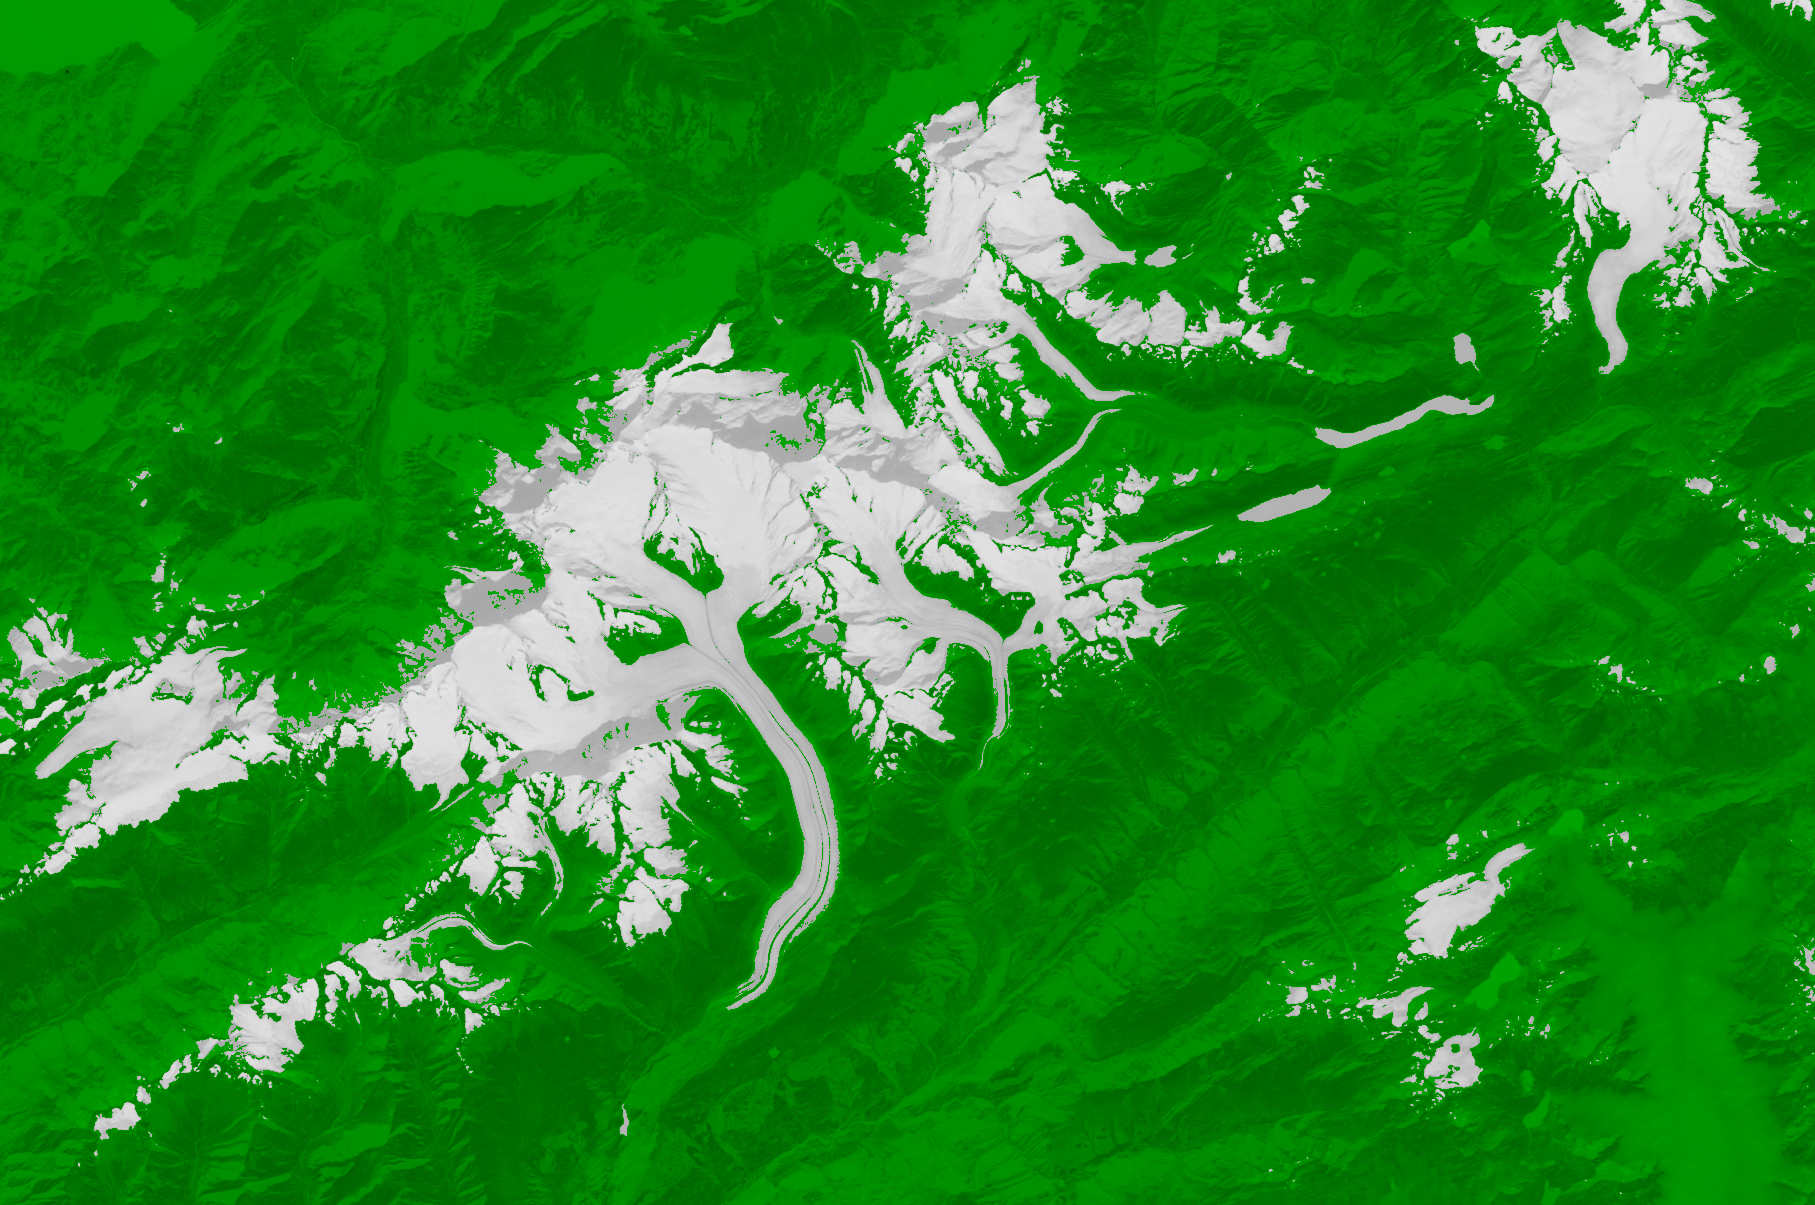
\includegraphics[width=\linewidth]{../images/LC81950282014271_ndsi.png}
	\caption{NDSI image of scene LC81950282014271, Jungfrau-Aletsch-Bietschhorn glacier.}
	\label{fig:ndsi}
	\end{figure}

	\par The image is colour coded in order to enhance the difference between pixels which are considered either snow or ice (white), and the rest of the terrain (green).

	% ==================================================================================

	\section{Alignment}
	\label{seq:alignment_functional}
	
	\par Landsat's trajectory orbiting Earth is not fully precise, therefore not all images will be pixel-to-pixel aligned, which is a problem for image processing. Since we want to track each pixel's movement, we must be sure that its coordinates in the image do not change between any two given scenes. Figure~\ref{fig:unaligned} highlights the misalignment from scene between scenes LC81950282013316 and LC81950282013364, as an example.
	
	\begin{figure}[h!]
	\centering
	\centering
	\includegraphics[width=\linewidth]{../images/unaligned_LC81950282014271LGN01_and_LC819502820162245LGN01.png}
	\caption{Overlapped unaligned green band of scene LC81950282014271LGN01 and reference LC819502820162245LGN01.}
	\label{fig:scene_unaligned}	
	\end{figure}

	\par Since the bands we work with have a spacial resolution of 30 meters, which means that each pixel in the image represents 30 meters. Even with a misalignment of just 50 pixels we would end up with a 1.5 km difference between two scenes. Tracking pixels through the image without aligning them first would mean that we could never be sure that what we are looking at is indeed the same location. We have used different approaches on alignment which will be described in Section~\ref{seq:alignment_implementation}. Figure~\ref{fig:scene_aligned} highlights the alignment corrected scene from Figure~\ref{fig:scene_unaligned}. 
	
	\begin{figure}[h!]
		\centering
		\includegraphics[width=\linewidth]{../images/aligned_LC81950282014271LGN01_and_LC81950282016245LGN01.png}
		\caption{Overlapped aligned green band of scene LC81950282014271LGN01 and reference LC819502820162245LGN01.}
		\label{fig:scene_aligned}
	\end{figure}

	\subsubsection{NDSI's Optical Flow}
	\label{seq:ndsi_motion_matrix}
	
	\par Since our dataset represents a \textbf{time series of satellite images}, as described in Section~\ref{seq:landsat8_section}, we thought that in order to generate a new image of this series, we could extract the \textbf{motion of each pixel} from one scene to another. This information could then be applied between any two consecutive (date-wise) scenes from the set and we could update a pixel's coordinates based on the value its motion vector and store it in a new image.
	
	\par Extracting the motion vectors between two consecutive frames can be achieved by calculating their optical flow. \textbf{Optical flow} is defined as the motion of objects between consecutive frames of sequence, produced by the relative movement between the object and camera. By using computer vision algorithms which calculate the optical flow of two scenes, we could track the motion of melting glaciers across them in order to estimate their current velocity and possibly \textbf{predict their position} in the next frames \cite{opticalflow}.
	
	\begin{figure}[h]
		\centering
		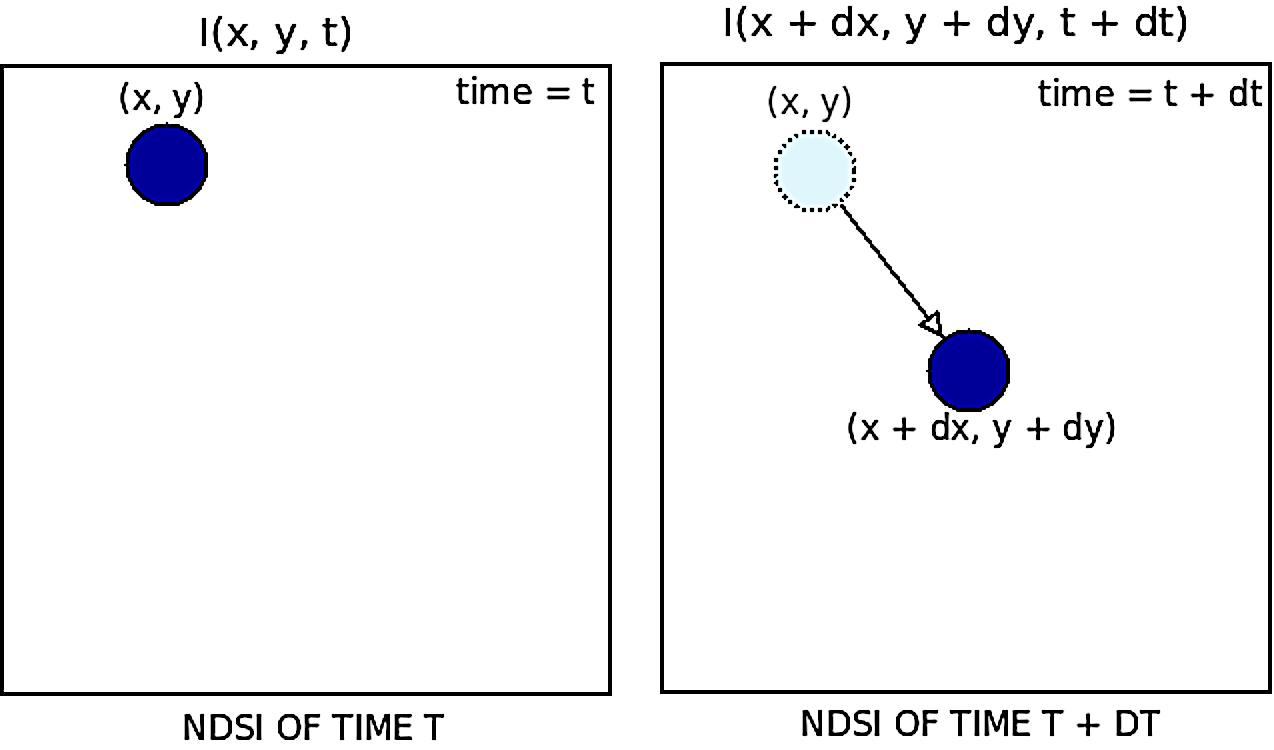
\includegraphics[scale=0.6]{../images/optical_flow_schema.png}
		\caption{Optical flow problem visualisation.}
		\label{fig:optical_flow_example}
	\end{figure}
	
	\par Figure~\ref{fig:optical_flow_example} emphasizes the problem visually, where we can express an image as a \textbf{function of space}, with the coordinates \textbf{\((x, y)\)}, and \textbf{time} \textbf{\(t\)}. If we take the first image\textbf{ \(I(x, y, t)\)} and we move its pixels by a distance of \textbf{\(dx, dy\)} over a timestamp \textbf{\(dt\)}, we obtain the new image as follows: \textbf{\(I(x + dx, y + dy, t + dt)\)} \cite{orb}.
	
	\par There are multiple types of optical flow algorithms, but for the purpose of our thesis, we have chosen the \textbf{dense optical flow} one, specifically \textbf{Gunnar Farneback's}. Even if dense implementations have higher cost we chose to make this trade mainly because it calculates the motion for each pixel of the frame and it also has a higher accuracy \cite{orb} compared to methods such as Lucas-Kanade (sparse) \cite{lukas}.
	
	\par We have used optical flow as a tool to generate \textbf{distance vectors} based on motion between the NDSI(\(time=t\)) and NDSI(\(time=t + dt\)), as it can be seen in Figure~\ref{fig:optical_flow}. These vectors will be used in order to create the \textbf{motion predicted NDSI}. 
	
	\begin{figure}[h!]
		\centering
		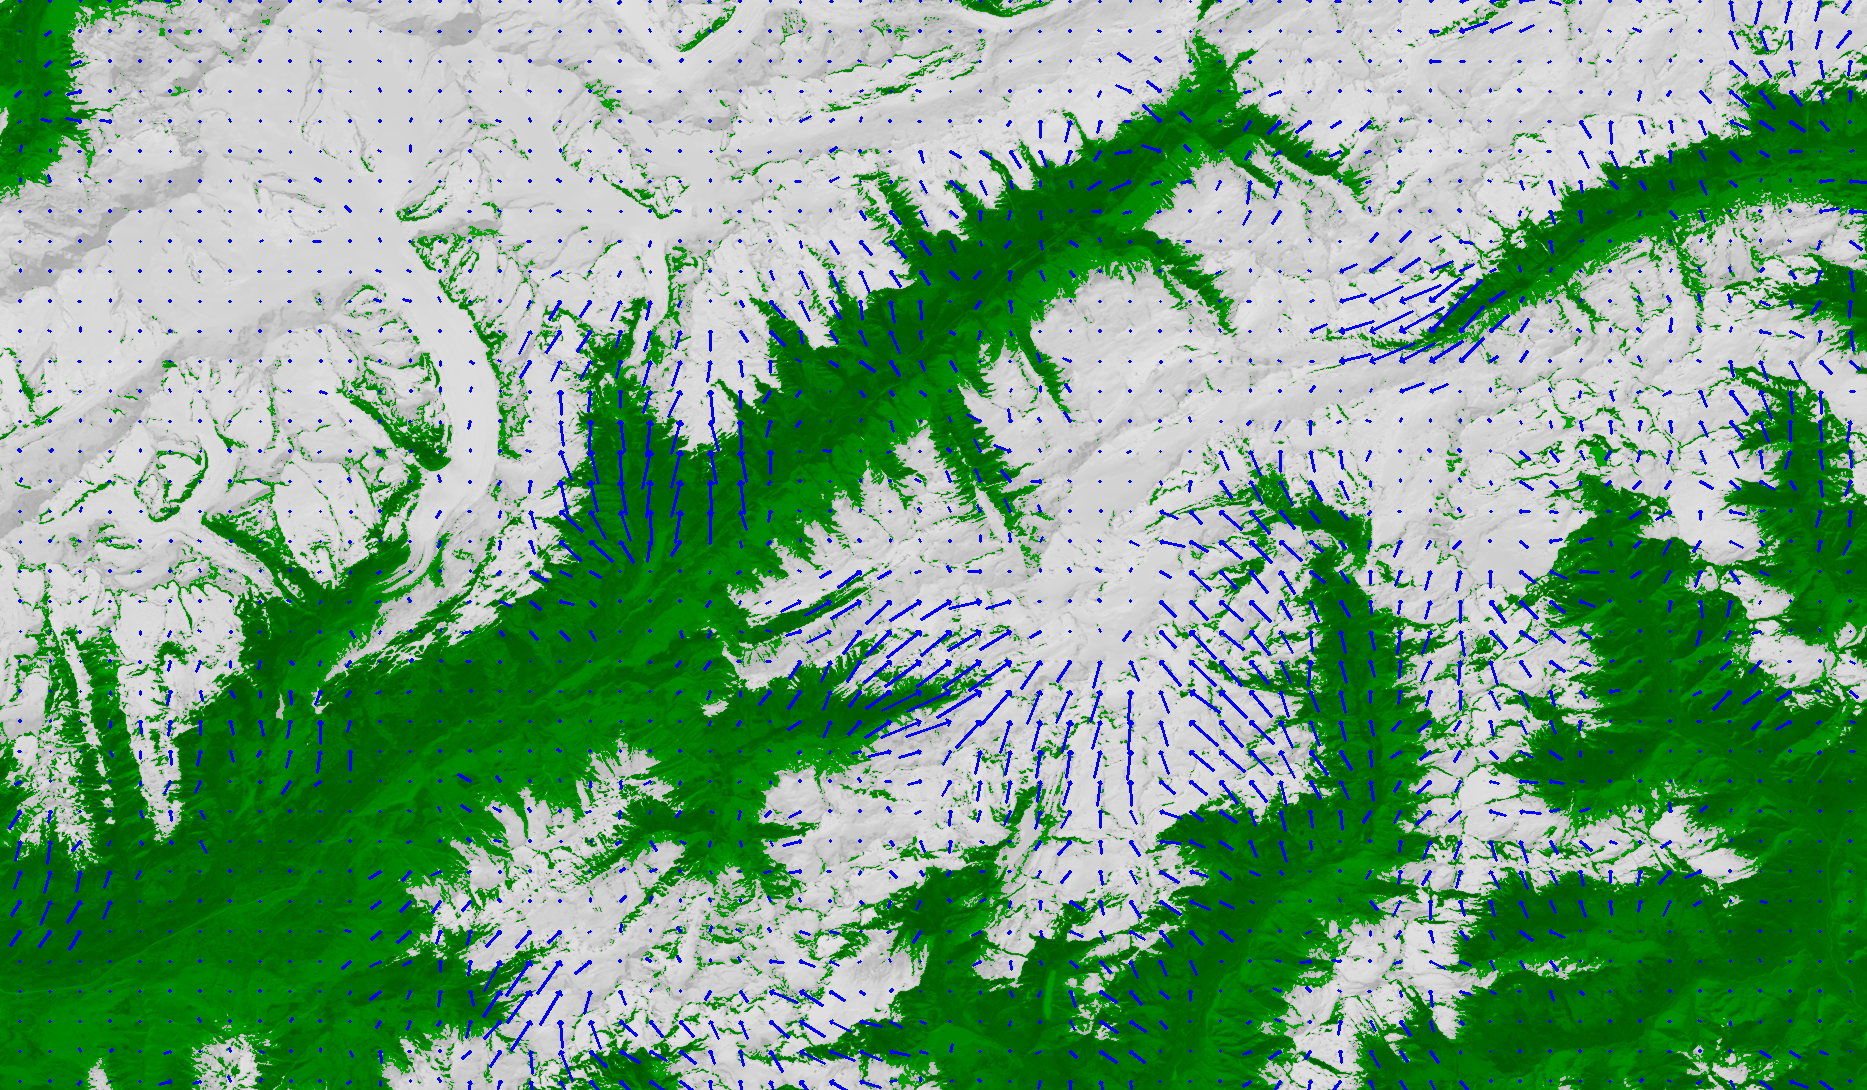
\includegraphics[scale=0.32]{../images/LC81940282015363LGN02_NDSI_vectros_small.png}
		\caption{Optical flow overlayed motion vectors.}
		\label{fig:optical_flow}
	\end{figure}

	\subsubsection{Motion Predicted NDSI}
	\label{seq:motion_ndsi_functional}
	
	\par Whilst optical flow allows us to see movement of the ice front which already happened in the past, we wanted to use this information and apply it on the most recent images such that we can estimate further glacier movements.

	\par We obtain the motion predicted generated NDSI by relocating each pixel value from the NDSI(\(time=t + dt\)) to a \textbf{predicted location}. For now, this location is generated by adding the distance vectors obtained by optical flow as described in Section~\ref{seq:motion_ndsi_implementation} to the pixels of the same image, therefore shifting them by twice as much as they originally did, in their respective directions, as it can be observed in Figure~\ref{fig:motion_generated_schema}. More methods of calculating the predicted location can be found in Section~\ref{seq:future_development}.
	
	\begin{figure}[h!]
		\centering
		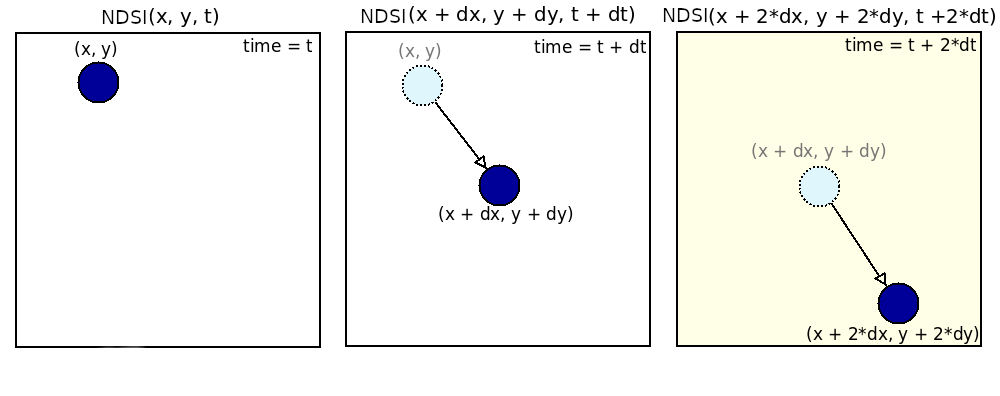
\includegraphics[scale=0.5]{../images/motion_generated_schema.png}
		\caption{Motion generated NDSI algorithm.}
		\label{fig:motion_generated_schema}
	\end{figure}

	\par By applying this function to each pixel of the NDSI (\(t + dt\)) image and by making some adjustments which are further described in Section~\ref{seq:motion_ndsi_implementation}, for scene LC81940282015363LGN02, we have generated the motion predicted NDSI as shown in Figure~\ref{fig:motion_predicted_image}. The ice coverage for the generated image is 5.0099\% while the one for the actual NDSI(\(time=t+dt\)) is 5.3066\%.
	
	\begin{figure}[h!]
	\centering
	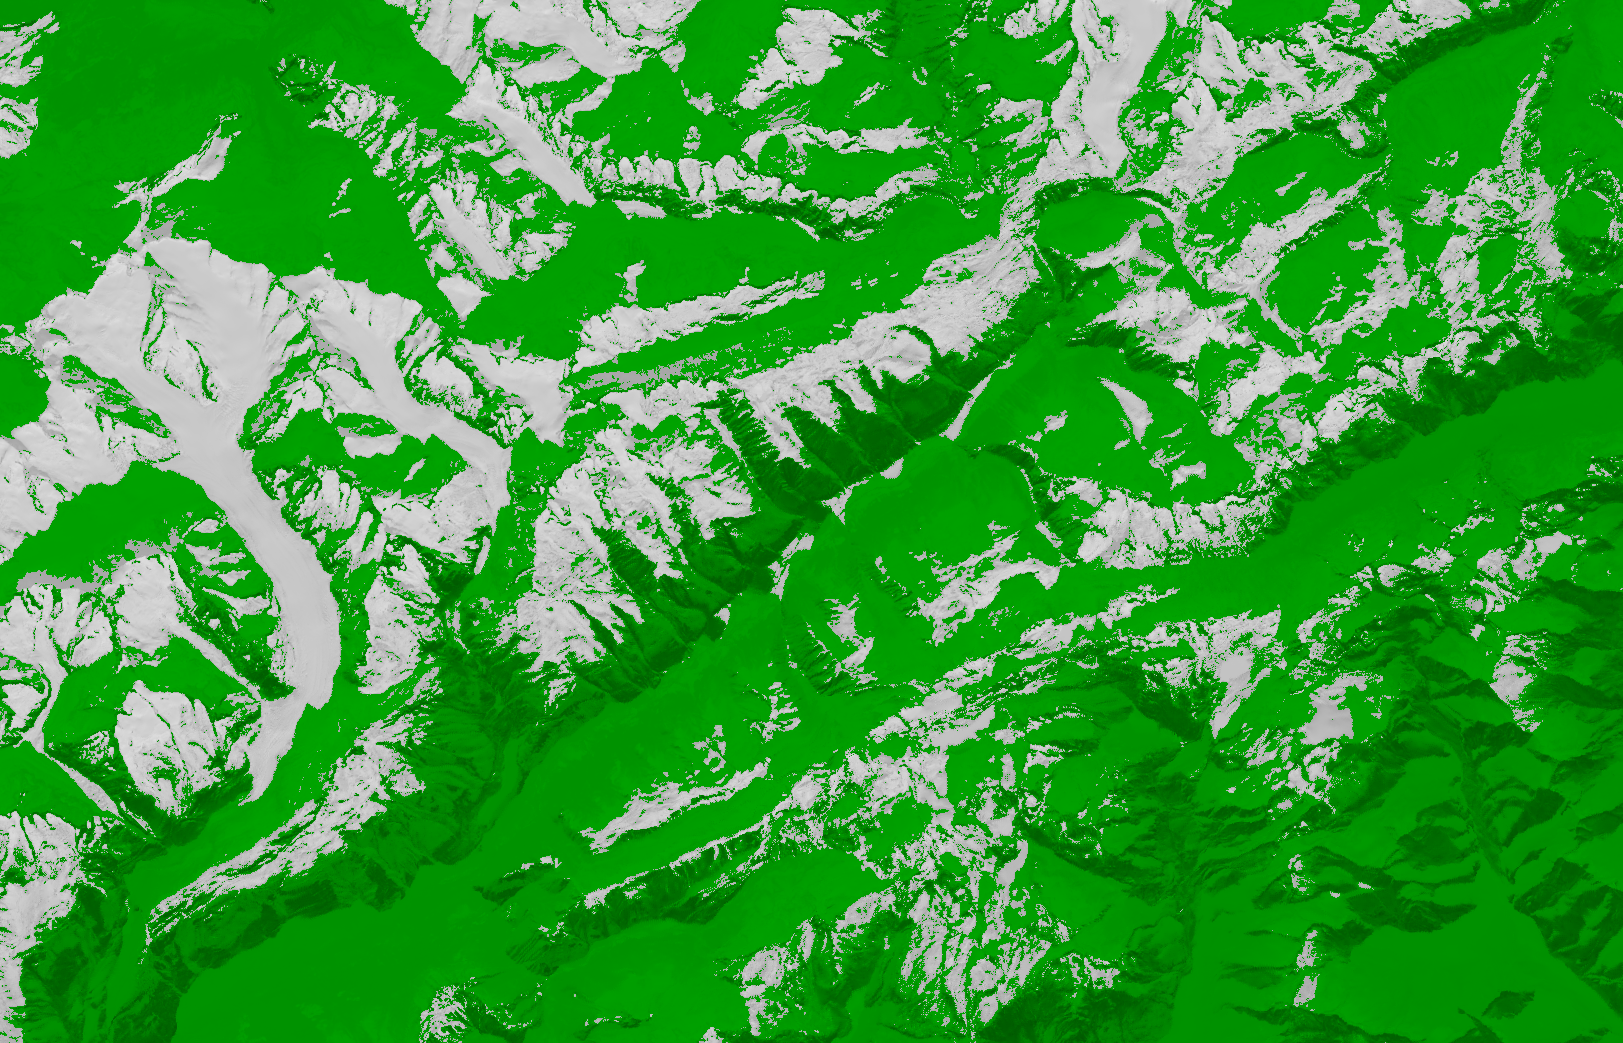
\includegraphics[width=\linewidth]{../images/LC81940282015363LGN02_motion_predicted.png}
	\caption{Motion generated NDSI for scene LC81940282015363LGN02.}
	\label{fig:motion_predicted_image}
	\end{figure}

	In order to better visualise the differences between the two images, they have been overlapped and colourized such that orange areas of snow that are predicted to melt, while blue represents areas which are predicted to develop snow build up.
	
	\begin{figure}[h!]
		\centering
		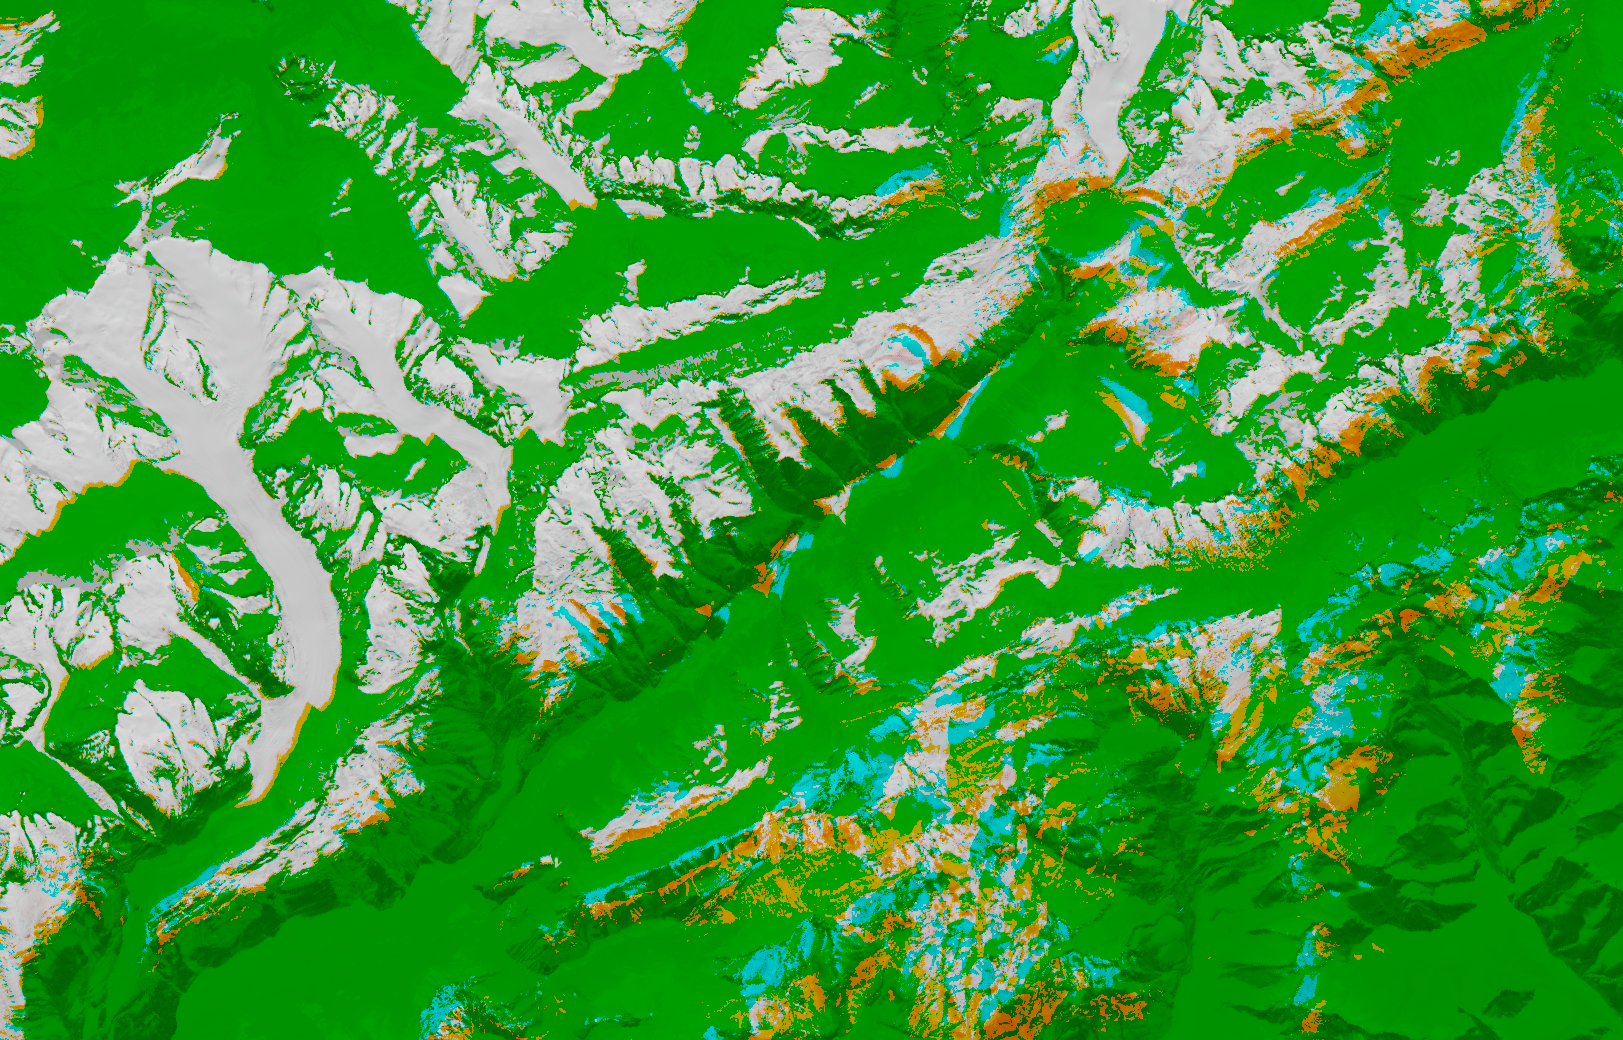
\includegraphics[width=\linewidth]{../images/LC81940282015363LGN02_motion_predicted_overlay.png}
		\caption{Overlapped motion generated NDSI for scene LC81940282015363LGN02.}
		\label{fig:overlapped_motion_predicted_image}
	\end{figure}


	% =========================================================================	
	\newpage{}
	\section{Graphical User Interface}
	\label{seq:gui}
	
	\subsection{Search and Download}
	\label{seq:search_download}

	% =========================================================================
	\newpage{}
	\chapter{Design and Implementation}
	\label{cha:design_and_implementation}
	
	\par The design of the application will be discussed while focusing on two different aspects:
	
	\begin{itemize}
		\item \textbf{search and download}
		\item \textbf{processing}
	\end{itemize}

	\par The first section is optional and can be run independently from the processing, since the user can have an already created database of images. However, we have focused on simplifying the process of satellite imagery downloading as described in \ref{seq:STAC} through using the sat-search library as a helper for searching and downloading assets. More information on querying can be found in \ref{seq:sd_implementation}. 
	Given an existing set of data, the next step is to pass the root folder which contains the glacier directories to the processing unit, also designed as a plug-in mechanism which will trigger the graphical user interface to pop up and allow for the processing options to appear. More information on this section can be found at \ref{seq:processing}. From there, one can start processing by simply making use of the predefined buttons described in \ref{seq:gui}.
	
	% =========================================================================
		
	\section{Search and Download}
	\label{seq:sd_implementation}
		
	\par Searching as well as downloading have been implemented on top of the sat-search library and it is used directly from the command line interface by running the script described in Section~\ref{seq:search_download}.
	
	\par As an input we will be using a CSV file which will have the form as described in Section~\ref{seq:wgi}. Mainly we will need just four attributes to be specified for each desired glacier in order to create a query for searching, as follows: \textit{wgi\_glacier\_id, glacier\_name, lat and lon}.
	
	\par The CSV file will be intercepted by the \textbf{Download } class and sent for processing row by row (glacier by glacier) to the \textbf{GlacierFactory} class. This one is responsible for parsing each row of the input CSV file and transforming the information in \textbf{Glacier} objects, which will be passed back to the \textbf{Download} class.
	
	\par Using the newly created Glacier object we can construct its \textbf{search query} by calculating its bounding box, specifying the asset collection from which we request data and setting other parameters (maximum allowed cloud coverage, in our case). Listing~\ref{lst:query} represents an example of querying for glacier Belvedere, with the following parameters set in the CSV file: \textit{"IT4L01211009","BELVEDERE","45.942","7.908"}.
	
	\begin{lstlisting}[caption={Search query created by sat-search},label={lst:query},language=Bash]
		{"page": 1, "limit": 170, "bbox": [7.907990000000001, 45.94199, 7.90801, 45.94201], "query": {"eo:cloud_cover": {"lt": 10}}, "collection": "landsat-8-l1"}
	\end{lstlisting}

	\par The result of each glacier query will be automatically saved in a \textbf{JSON file} which is used as a data buffer between the search and download. The downloader takes each JSON file generated by the search engine and sends the command for getting that asset.
	
	\par The technical specifications of the Download, GlacierFactory and Glacier classes can be found in Figure~\ref{fig:sd_diagram}.
	
	\begin{figure}[h]
		\centering
		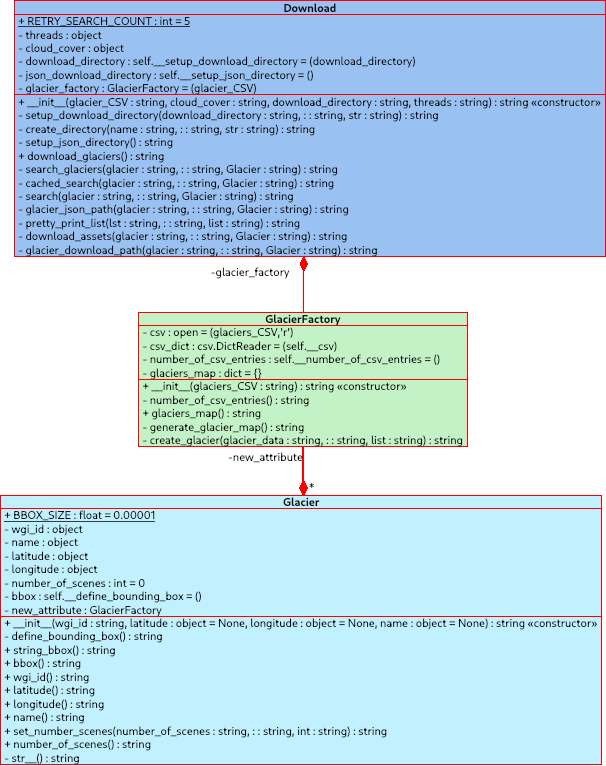
\includegraphics[scale=0.23]{../images/sd_diagram.png}
		\caption{Technical specifications of Download, GlacierFactory and Glacier classes.}
		\label{fig:sd_diagram}
	\end{figure}

	\paragraph{Data corruption verification}
	Both the searching and downloading functions are executed concurrently, since they are \textbf{time intensive} tasks. Each band has around 60 MB, which would make one scene approximately 360 MB. For the Belvedere glaciers, we found 78 scenes with a cloud coverage of 10\%. This means that the size of the entire glacier data will be around 28 GB. Given that one asset's size is quite large, it takes a lot of time to finish the download. In this time, even a small connection interruption might result in corrupted data files, which would interfere with processing. Therefore, we implemented an \textbf{extra security measure} in the sat-stac library which verifies whether a file with the same name already exists at the download location. If it does, its size will be compared to the size taken from the STAC-API servers. In case the two file sizes don't match, it means that the file got corrupted during download and it will be downloaded again. If the sizes match, the downloader will skip the file and continue when it finds one requested file which was not yet found on the disk, such that we do not end up unnecessarily overwriting the already existing files in case of failure.
	
	% =========================================================================

	\section{Processing}
	\label{seq:processing}
	
	\par Processing can be viewed as four different entities, as following:
	
	\begin{itemize}
		\item Image alignment;
		\item Normalized snow difference index;
		\item NDSI's motion matrix;
		\item Motion generated NDSI.
	\end{itemize}

	\par Before generating any images, we first need to make sure that the pixels between any two scenes are not misaligned. The details of the alignment process are described in Section~\ref{seq:alignment_implementation}. After we ensure that out images are fit, we move on to creating the normalized snow difference index image in order to enhance the ice through a set threshold (see Section~\ref{seq:ndsi_implementation}). We then create the matrix of pixel motions calculated between two consecutive (date-wise) scenes, process described in Section~\ref{seq:motion_matrix_implementation}. Based on the information of where each pixel has moved between two consecutive images, we can then create our future NDSI image by applying the motion vectors on each pixel from a scene. More details on the design and implementation of this part can be found in Section~\ref{seq:motion_ndsi_implementation}.
	The normalized snow difference index image will be computed for each scene as described in Section~\ref{seq:ndsi_functional}.
	
	%========================================================================================
	
	\subsection{Alignment}
	\label{seq:alignment_implementation}\
	
	\par In order to keep a high level of abstraction, we have split each scene into aligned and unaligned: Scene and AlignedScene objects. These and their children are created when crawling through the glaciers directory, specifically for each region of interest. However, aligning all the images when crawling would result into a lot of idle time for the user when starting the application and it would not be overall feasible to do so. Therefore, a scene is aligned only when it is specifically being selected in the graphical user interface (or when another entity needs it, such as optical flow and image generation). By doing this, we ensure that there is no unnecessary extra waiting time for each scene that we have when powering up the interface.
	
	\par As for the actual alignment, we have used an algorithm which \textbf{collects features} from each band of a scene and tries to match them with a given reference one's features. The obtained \textbf{matches} can be then used to create an \textbf{affine transformation matrix} which specifies by how much did the current image \textbf{rotated and translated} in comparison to its reference. The affine transformation matrix will be then applied to the current image by a \textbf{warping} algorithm with the goal of ensuring as much as possible that there is no misalignment between any pixel of two different images from the same time series. Section~\ref{seq:alignment_algorithm} describes more technically how we built this and what were the computer vision algorithms used for that matter. Figure~\ref{fig:alignment_diagram} contains the technical details of each class which takes part into the alignment process.
	
	\begin{figure}[h!]
		\centering
		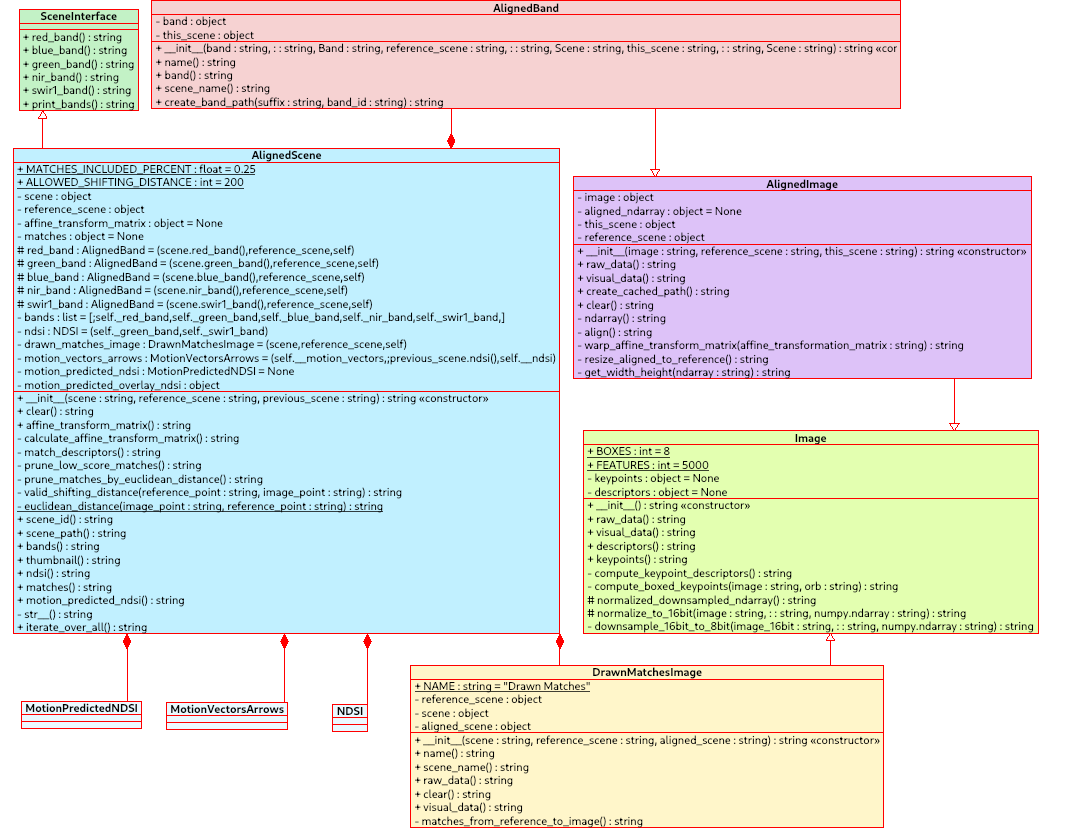
\includegraphics[scale=0.45]{../images/alignment_diagram.png}
		\caption{Technical diagram for the SceneInterface, AlignedScene, AlignedBand and Image classes.}
		\label{fig:alignment_diagram}
	\end{figure}

	\subsubsection{Alignment algorithms}
	\label{seq:alignment_algorithm}
	
	\par As we have seen in Section~\ref{seq:landsat8_section}, the Landsat 8 satellite does not have a perfect trajectory, which results into misaligned images. These changes are not obvious to the naked eye from scene to scene, but overlapping two scenes highlights this problem, as we can see in Figure~\ref{fig:unaligned}. Even so the scenes are almost similar, which means that aligning them does not prove to be very hard and it is done by using a strong \textbf{keypoint detection algorithm} which in our case detects edges formed by mountains and other geographical features present in the scenes. The \textbf{computer vision algorithms} used for this are \textbf{ORB (Oriented FAST and Rotated BRIEF)}, \textbf{Harris Corner Detector} and \textbf{RANSAC (Random Sample Consensus)} and they are applied on the raw 16bit grayscale image.
	
	\par \textbf{ORB} represents a fusion between the features from accelerated segment test (\textbf{FAST}) keypoint detector and binary robust independent elementary features (\textbf{BRIEF}) descriptor. The FAST detector finds keypoints in the image and uses Harris corner measure to select the a number of top points from the list (25\%, in our case) \cite{orb}. In order to use the detector we must first normalize and downsample the 16bit raw image to 8 bit, as it is required by ORB. Each keypoint is then represented by a circle of 16 pixels. The descriptors must then identify these keypoints and pair with each other.
	We compute for each scene its \textbf{keypoints and descriptors} taken from \textbf{each band}, in order to increase the precision of alignment later on. Also, since we are working with satellite imagery there might be cases when the algorithm only finds keypoints in a small part of the image, resulting in erroneous distortion. \textbf{Splitting} the image into multiple boxes and applying the orb detect algorithm on each separate part of the image proved to solve this problem and create much better results. 
	
	\par After ensuring that we have good enough keypoints we will be aligning each scene with its reference by simply comparing the keypoint-descriptor pairs between the two scenes and checking which are equal. If two pairs are found to be equal, it means that the algorithm has found the same feature in both images and can calculate by how much it \textbf{rotated and shifted}. However, not all of these matches represent good results in our case, since the trajectory Landsat 8 can vary. We have found that selecting only \textbf{5000 keypoints} in the \textbf{top 25\% matches} from the total yielded in the better results overall. We then set the \textbf{maximum allowed shifting euclidean distance} between any two pixels to be at most 200, so 6km on the map, therefore getting rid of outlier matches based on the distance.
	
	\par The \textbf{matches} from the reference and image to be aligned will be used alongside the \textbf{Random Sample Consensus (RANSAC)} algorithm in order to create the \textbf{affine transformation matrix} using the cv2 library. RANSAC, proposed by Fischler and Bolles \cite{ransac}, is a general parameter estimation approach designed to handle a large proportion of outliers in the input data \cite{ransac2}. After we have the transformation matrix, we can \textbf{warp} it on the image to be aligned in order to get the result. 
	%========================================================================================
	
	\subsection{Normalized Snow Difference Index}
	\label{seq:ndsi_implementation}
	
	\begin{figure}[h!]
		\centering
		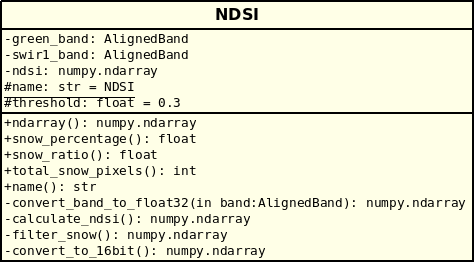
\includegraphics[scale=0.6]{../images/ndsi_diagram.png}
		\caption{Technical diagram for the NDSI class.}
		\label{fig:ndsi_diagram}
	\end{figure}

	\par The NDSI is generated by using the Formula~\ref{eq:ndsi_formula} described in section \ref{seq:ndsi_functional} on the green and shortwave infrared bands from a specific scene. Each band pixel is converted to \textbf{float32} in order to increase the \textbf{precision} of calculation; as each band is read as a n-dimensional array we can use numpy's optimised processing for generating the NDSI index image, since it converts the data and runs on native code rather than going through Python's interpretor. We then \textbf{filter} the generated image such that everything which is snow-free land will be -1 (\textbf{black}), but this is only applied for better visual analysis. In the background, we work with the full range of the image for better precision, which is the raw image. 
	\par Figure~\ref{fig:ndsi_diagram} holds the technical diagram for the NDSI.

	%========================================================================================

	\subsection{NDSI's Optical Flow}
	
	\begin{figure}[h!]
		\centering
		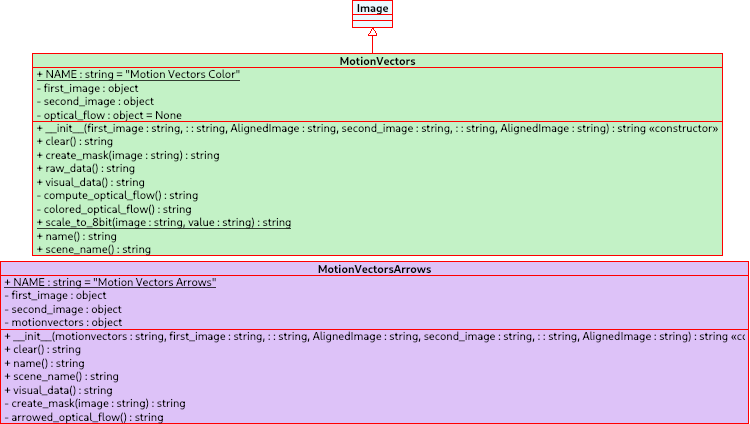
\includegraphics[scale=0.6]{../images/motion_vectors_diagram.png}
		\caption{Technical diagram for the MotionVectors class.}
		\label{fig:motion_vectors_diagram}
	\end{figure}

	\par As described in Section~\ref{seq:motion_ndsi_implementation}, in order to determine the motion vector for each pixel between two images, we have used \textbf{Gunnar Farneback's} algorithm for dense optical flow calculation, implemented by the \textbf{OpenCV} library. The MotionVectors class takes as input two NDSI images.
	
	\par Since the NDSI images have been aligned, depending on the affine transformation matrix, they will not overlap perfectly any more, resulting in \textbf{artifacts at their borders}. Applying optical flow by using two NDSI images as such would result in highly distorted motion vectors at the borders. For fixing this, we have created a \textbf{mask} from each image such that both of them are cropped with the mask of the other. This results in losing a small number of pixels at the borders which could not be taken into consideration anyway.
	
	\par In addition to the two NDSI image inputs, we have used the \textbf{optical flow algorithm} with the \textbf{parameters} specified in Listing~\ref{lst:opticalparameters}. We have used a \textbf{pyramid scale of 0.5} and \textbf{6 pyramid levels} having in mind that the images that we work with are large. By choosing this combination of parameters, we state that at each level, the image is going to be reshaped at half the size of the previous one; therefore the area of search for motion is small enough such that the optical flow is able to track movement.  

	\begin{lstlisting}[caption={Optical flow parameters},label={lst:opticalparameters},language=Python]
		cv2.calcOpticalFlowFarneback(..., pyr_scale=0.5, levels=6, winsize=15, iterations=3, poly_n=5, poly_sigma=1.2, flags=0)
	\end{lstlisting}

	\par After our images are perfectly overlaid, we can give them as inputs to the optical flow algorithm. The result of this will be the computed \textbf{motions} for each pixel, represented as a tuple of the \textbf{distance} that its coordinates moved from one frame to another. Specifically, as referring to Figure~\ref{fig:motion_generated_schema}, each item from the optical flow n-dimensional array will represent the \textbf{motion distance vector (\(dx, dy\))} as calculated between \textbf{NDSI(\(time=t\)) and NDSI(\(time=t + dt\))}.
	
	\par To be able to visually interpret the optical flow output, we have used a \textbf{colour coded image}. Colour intensity is directly proportional to the motion vector length, while its hue represents the direction of this vector, as represented in Figure~\ref{fig:hue_colour_wheel}.
	
	\begin{figure}[h!]
		\centering
		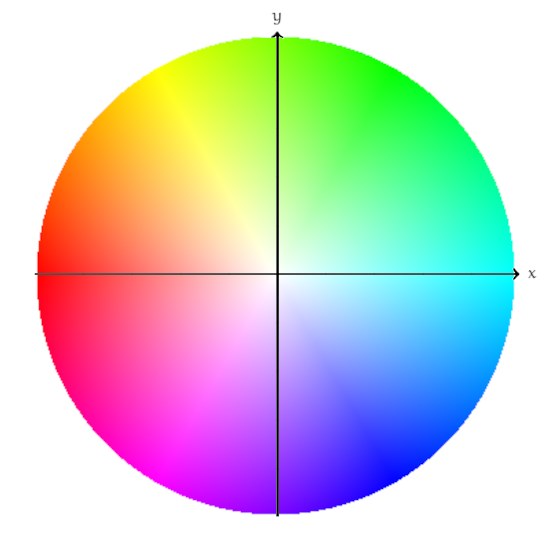
\includegraphics[scale=0.3]{../images/colorwheel.png}
		\caption{Hue representation of the optical flow.}
		\label{fig:hue_colour_wheel}
	\end{figure}
	
	\begin{figure}[h!]
		\centering
		\begin{minipage}{0.45\textwidth}
			\centering
			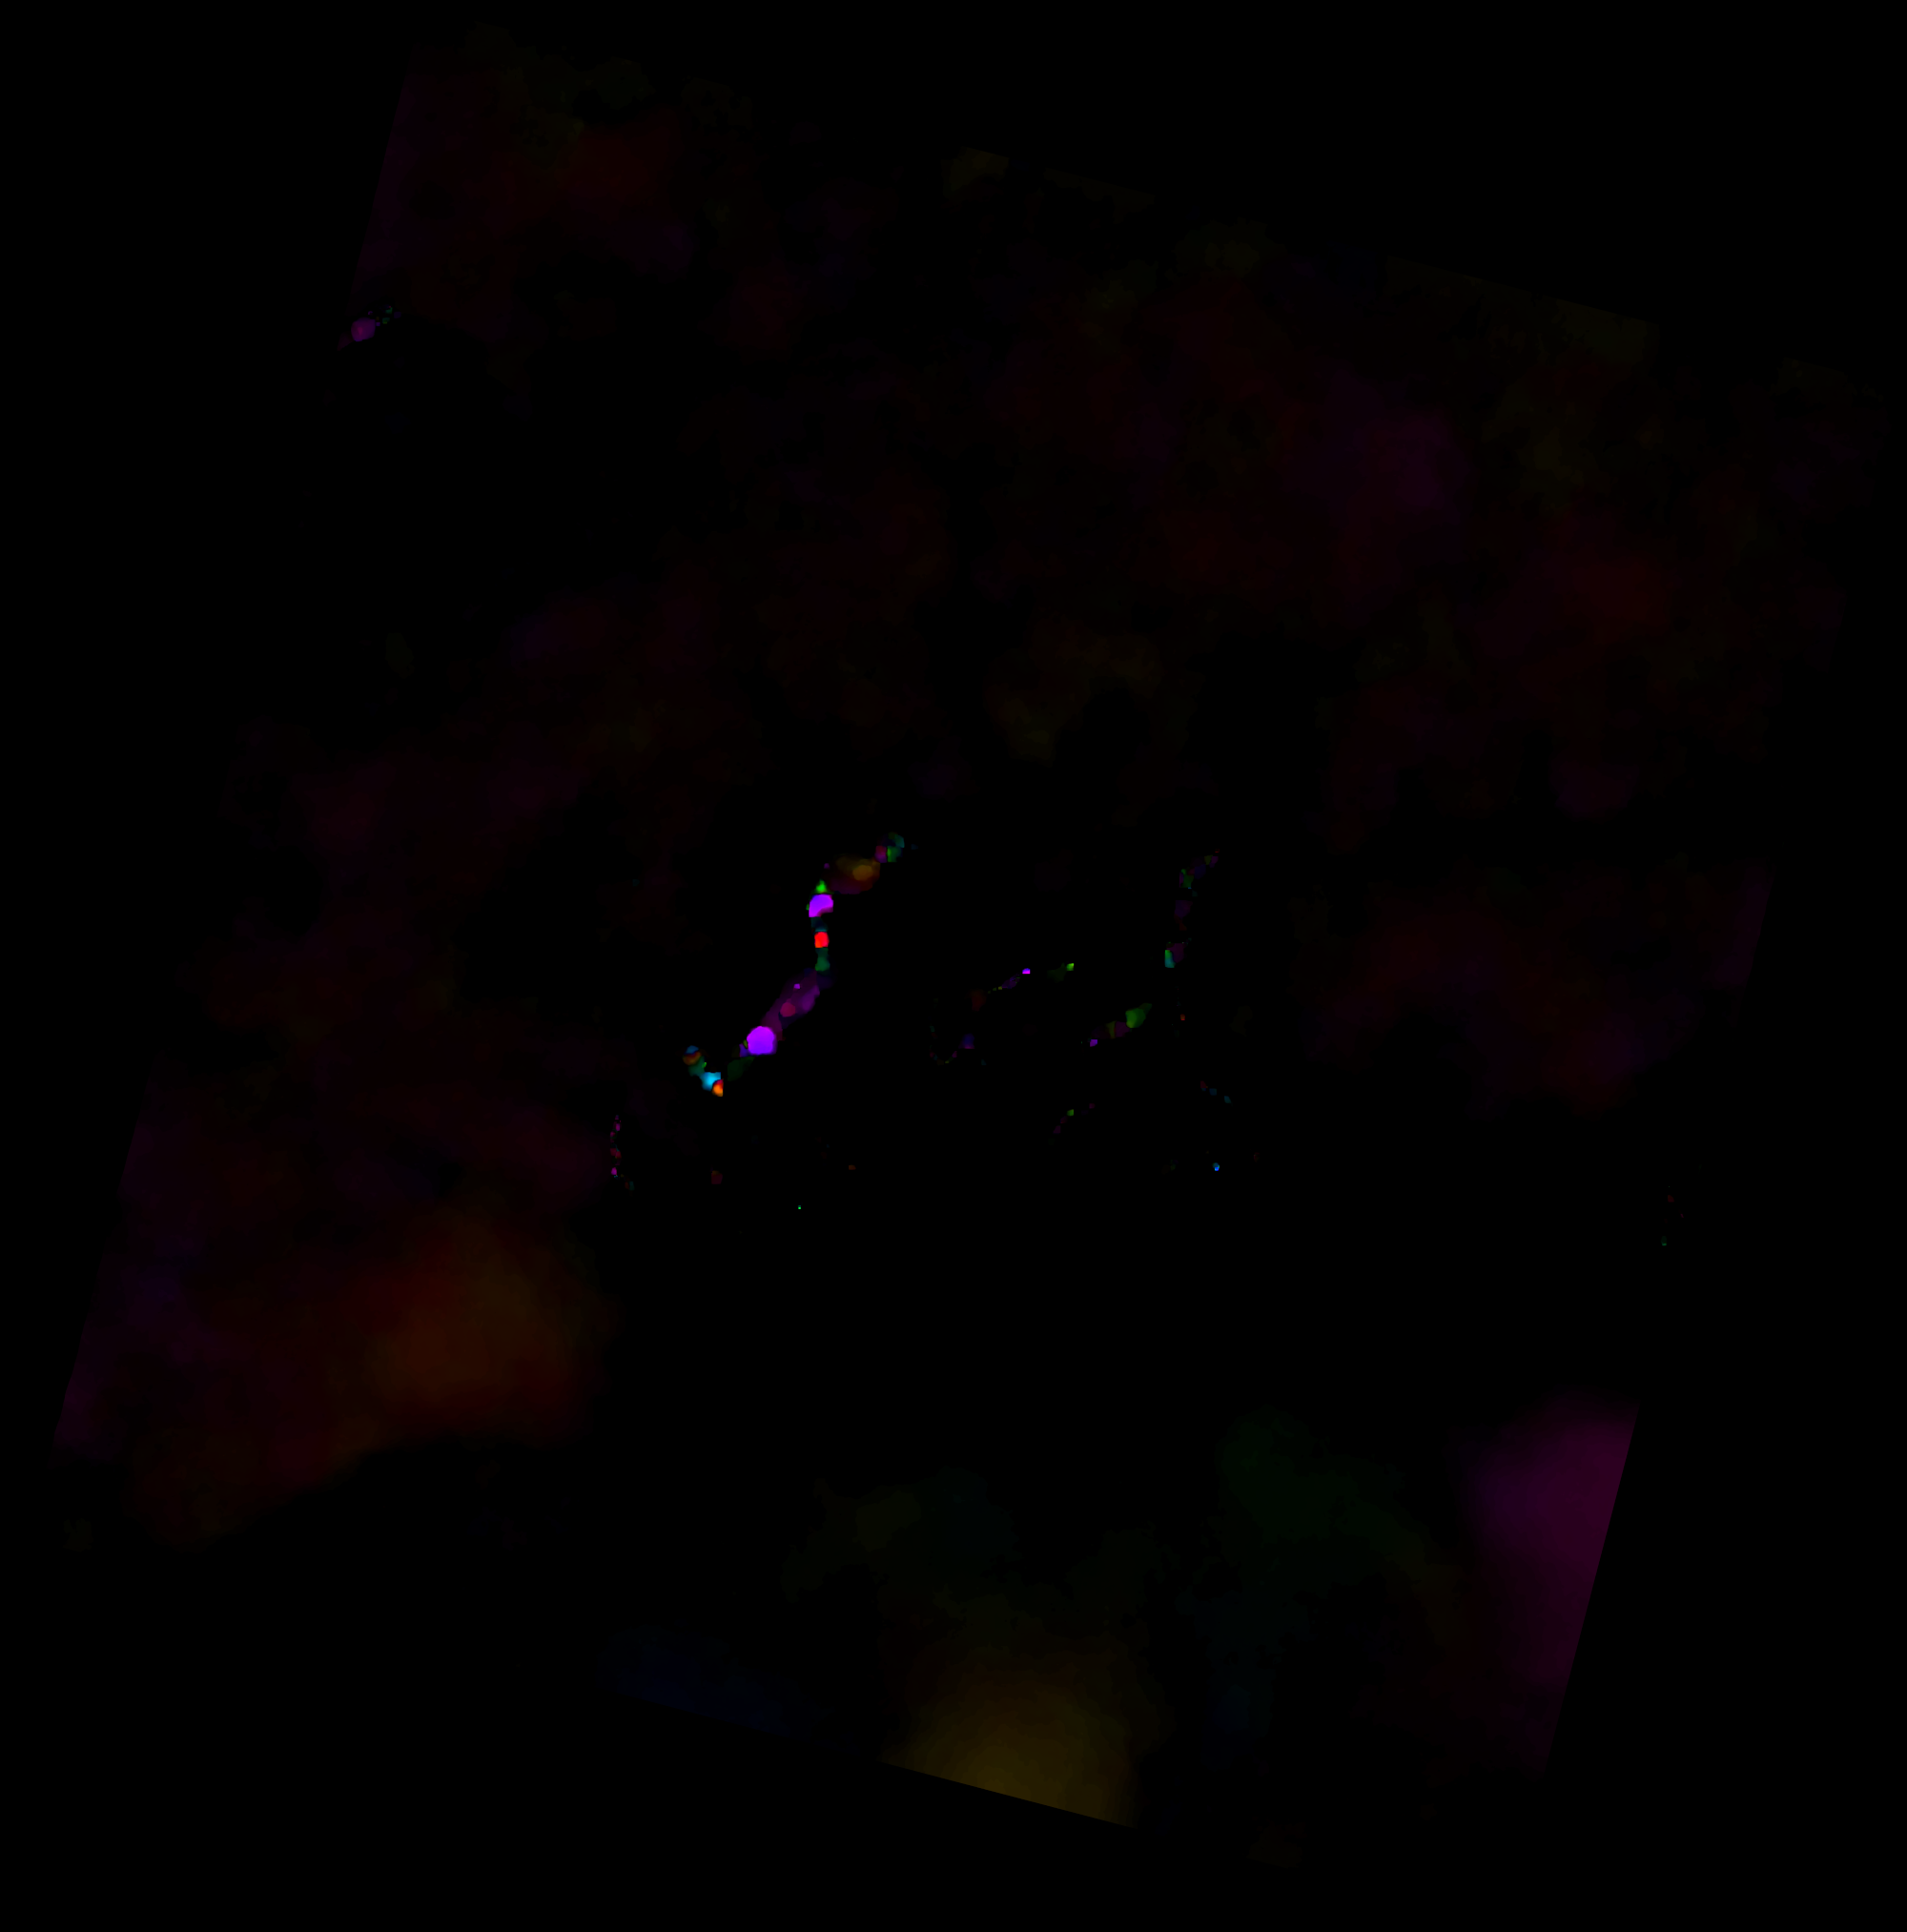
\includegraphics[width=\linewidth]{../images/LC81940282013341LGN01_Motion Vectros_color.png}
		\end{minipage}
		\begin{minipage}{0.45\textwidth}
			\centering
			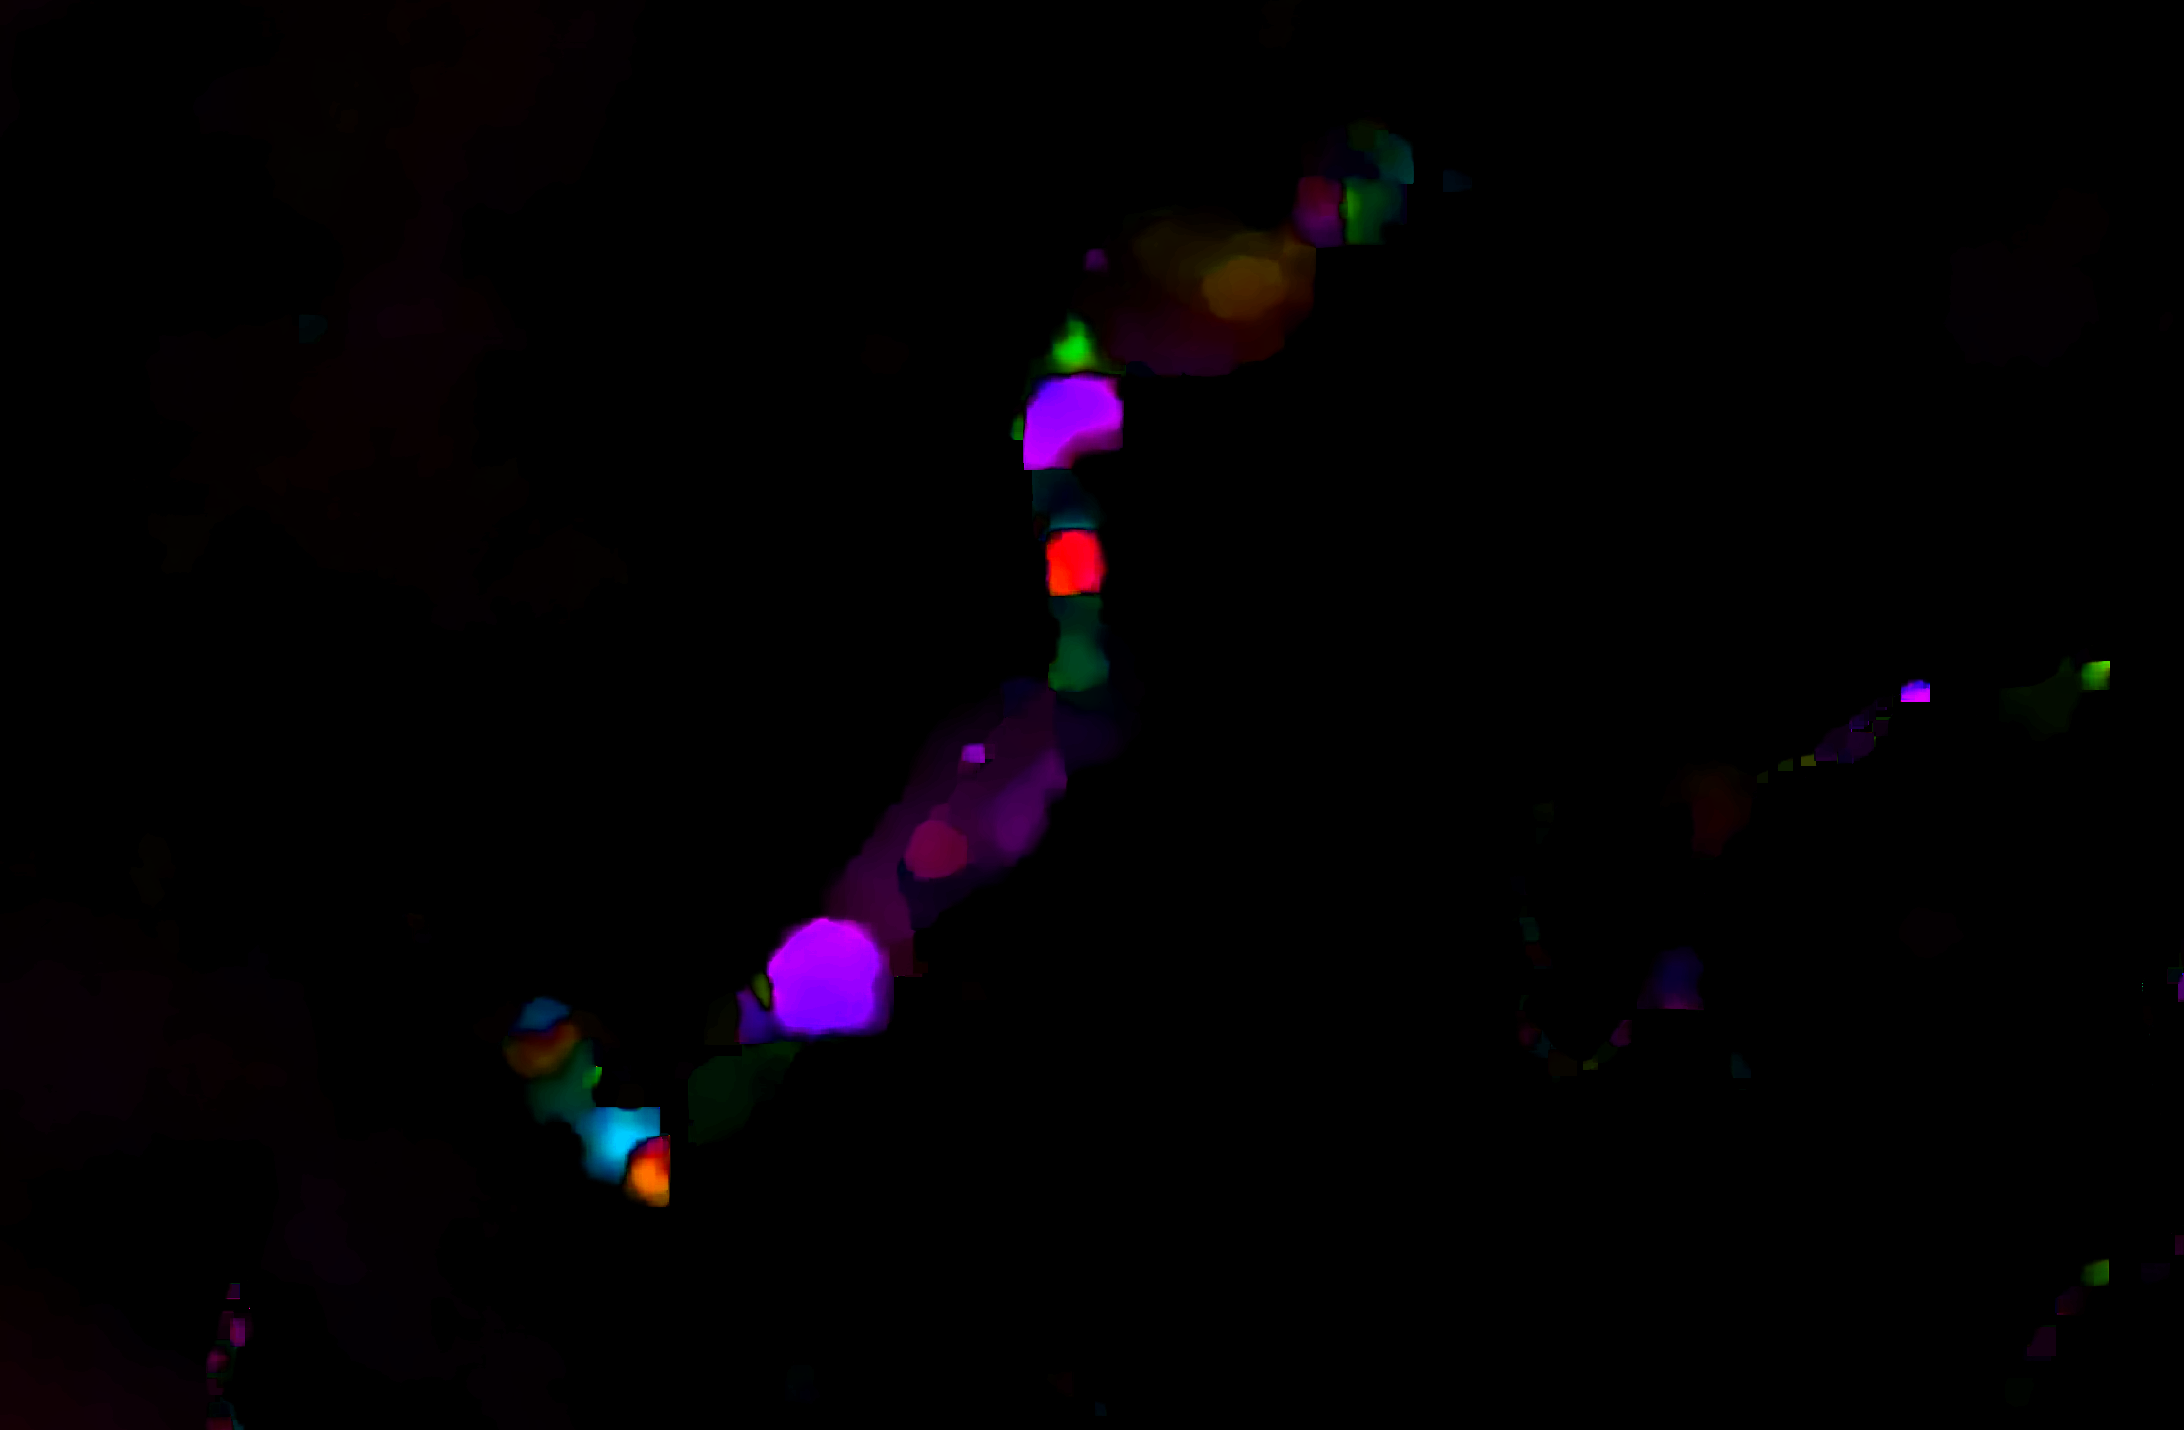
\includegraphics[width=\linewidth]{../images/LC81940282013341LGN01_Motion Vectros_color_small.png}
		\end{minipage}
		\caption{}
		\label{fig:NDSI}
	\end{figure}
	
	%========================================================================================

	\subsection{Motion Predicted NDSI}
	\label{seq:motion_ndsi_implementation}
	
	\par As means to put in practice what we described in Section~\ref{seq:motion_ndsi_functional}, we start by initialising a new numpy n-dimensional array based of the \textbf{shape} of the image \textbf{NDSI(\(time=t+dt\))}. The new array will be filled with the data generated by using the two required entities:
	
	\begin{itemize}
		\item \textbf{NDSI(\(time=t+dt\))};
		\item \textbf{motion vectors (\(dx, dy\))} extracted by optical flow.
	\end{itemize}
	
	\par Each \textbf{motion vector} (\(dx, dy\)) corresponds to the movement of a pixel from the NDSI(\(time=t+dt\)) image. We can use this information to \textbf{generate} the new \textbf{predicted position} (\(x + 2*dx, y + 2*dy\)) for each pixel of the NDSI(\(time=t+dt\)) image.
	
	
	\begin{algorithm}
			\SetKwInOut{Input}{Input}
			\SetKwInOut{Output}{Output}
			
			\underline{function generate} $(previous\_NDSI, motion\_vectors)$\;
			\Input{The NDSI(\(time=t+dt\) and the motion vectors generated by optical flow between NDSI(\(time=t\)) and NDSI(\(time=t+dt\))}
			\Output{The motion predicted NDSI(\(time=t+2*dt\)))}
			
			$motion\_predicted\_image \gets previous\_NDSI.shape$\;
			$width \gets NDSI.width()$\;
			$height \gets NDSI.height()$\;
			
			\For{$y$ in [$height, width$]}{
				\For{$x$ in [$height, width$]}{
					$dx \gets motion\_vectors[y][x][0]$\;
					$dy \gets motion\_vectors[y][x][1]$\;
	
					$new\_x \gets x + dx$\;
					$new\_y \gets y + dy$\;
					
					$motion\_predicted\_image[new\_y][new\_x] \gets previous\_NDSI[y][x]$\;
				} 
			}
			\Return{$motion\_predicted\_image$}\;

			\caption{Algorithm used for motion predicted image generation based on the optical flow vectors and NDSI(\(time=t+dt\))}
			\label{algo:change}
	\end{algorithm}
	
	\par As a first approach of populating the new image, we have simply \textbf{iterated} over all the pixels in the NDSI(\(time=t+dt\)) image and calculated their \textbf{new coordinates} based on their \textbf{motion vector} information, as it can be seen in Algorithm~\ref{algo:change}. Since this is an iterative approach, it does not scale for images as large as the ones we are using. On top of this, since we are using the Python language, which is an interpreted one, each operation has to go through an interpreter before being run. For very granular data processing this proves to be \textbf{inefficient}. For a typical image of 8543x8039 resolution, it takes as much as 10 minutes for generating the image on the machine that I have used (specifications at Section~\ref{seq:performance}).
	
	\par Since using the naive approach is not feasible in our application, we had to avoid iterating over the whole image in the first place. Therefore, instead of looping over each pixel in order to generate the values for the new image, we have made use of the \textbf{numpy} library to \textbf{heavily optimise} our data processing. By using numpy functions and vectorized operations directly instead of iterating we were able to improve the processing time by around 1700\%, bringing it down approximately from 10 minutes to 35 seconds.
	
	\par In the iterative approach, for each pixel we add its motion to its position such that we get its new location. These numbers can be computed ahead of time and transformed into arrays such that we only use numpy operations. By creating an \textbf{array of the initial coordinates} \(x, y\) and \textbf{adding the motion vectors} (\(dx, dy\)) array to it, we \textbf{generated the absolute coordinates} where each pixel from the NDSI image should be translated. By adding this modification we got rid of lines 5, 6, 7, 8, 9, 10 and 11 from the algorithm and replaced them with the code as it can be seen in Algorithm~\ref{algo:improved_generation}. The \(absolute\_coordinates\) and \(previous\_NDSI\) can be treated as a sparse array which is then densified using numpy capabilities.

	\begin{algorithm}
		\SetKwInOut{Input}{Input}
		\SetKwInOut{Output}{Output}
		
		\underline{function generate} $(previous\_NDSI, motion\_vectors)$\;
		\Input{The NDSI(\(time=t+dt\) and the motion vectors generated by optical flow between NDSI(\(time=t\)) and NDSI(\(time=t+dt\))}
		\Output{The motion predicted NDSI(\(time=t+2*dt\)))}
		
		$motion\_predicted\_image \gets previous\_NDSI.shape$\;
		$width \gets NDSI.width()$\;
		$height \gets NDSI.height()$\;
		
		$index\_array \gets [[[0, 0], [1, 0] ... [width, 0]$
		$[0, 1], [1, 1] ... [width, 1]$
		$...$
		$[0, height], [1, height] ... [width, height]]]$\;
		$absolute\_coordinates \gets motion\_vectors + index\_array$\;
		
		$motion\_predicted\_image[absolute\_coordinates] \gets previous\_NDSI$\;
	
		\Return{$motion\_predicted\_image$}\;
		
		\caption{Improved algorithm used for motion predicted image generation based on the optical flow vectors and NDSI(\(time=t+dt\))}
		\label{algo:improved_generation}
	\end{algorithm}

	\par The technical description of the MotionPredictedNDSI class can be found in Figure~\ref{fig:motion_predicted_diagram}.
	
	\begin{figure}[h!]
		\centering
		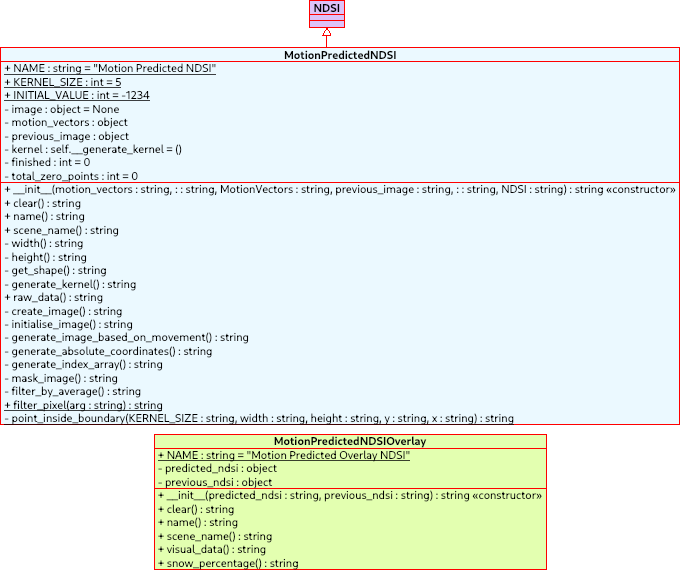
\includegraphics[scale=0.6]{../images/motion_created_diagram.png}
		\caption{Technical diagram for the MotionPredictedNDSI class.}
		\label{fig:motion_predicted_diagram}
	\end{figure}

	\par The function used to generate the predicted NDSI does not have a \textbf{one-to-one domain}, thus making it undefined for certain inputs. This results in a very \textbf{noisy} generated image, as it can be seen in Figure Figure~\ref{fig:unfiltered}. We have implemented a \textbf{filter} which uses the weighted average of the neighbouring pixels values to fill the missing ones. The detailed description of the implementation can be found in Section~\ref{seq:filter}.
	
	\subsection{Generated image filtering}
	\label{seq:filter}
	
	\begin{figure}[h!]
		\centering
		\begin{minipage}{0.45\textwidth}
			\centering
			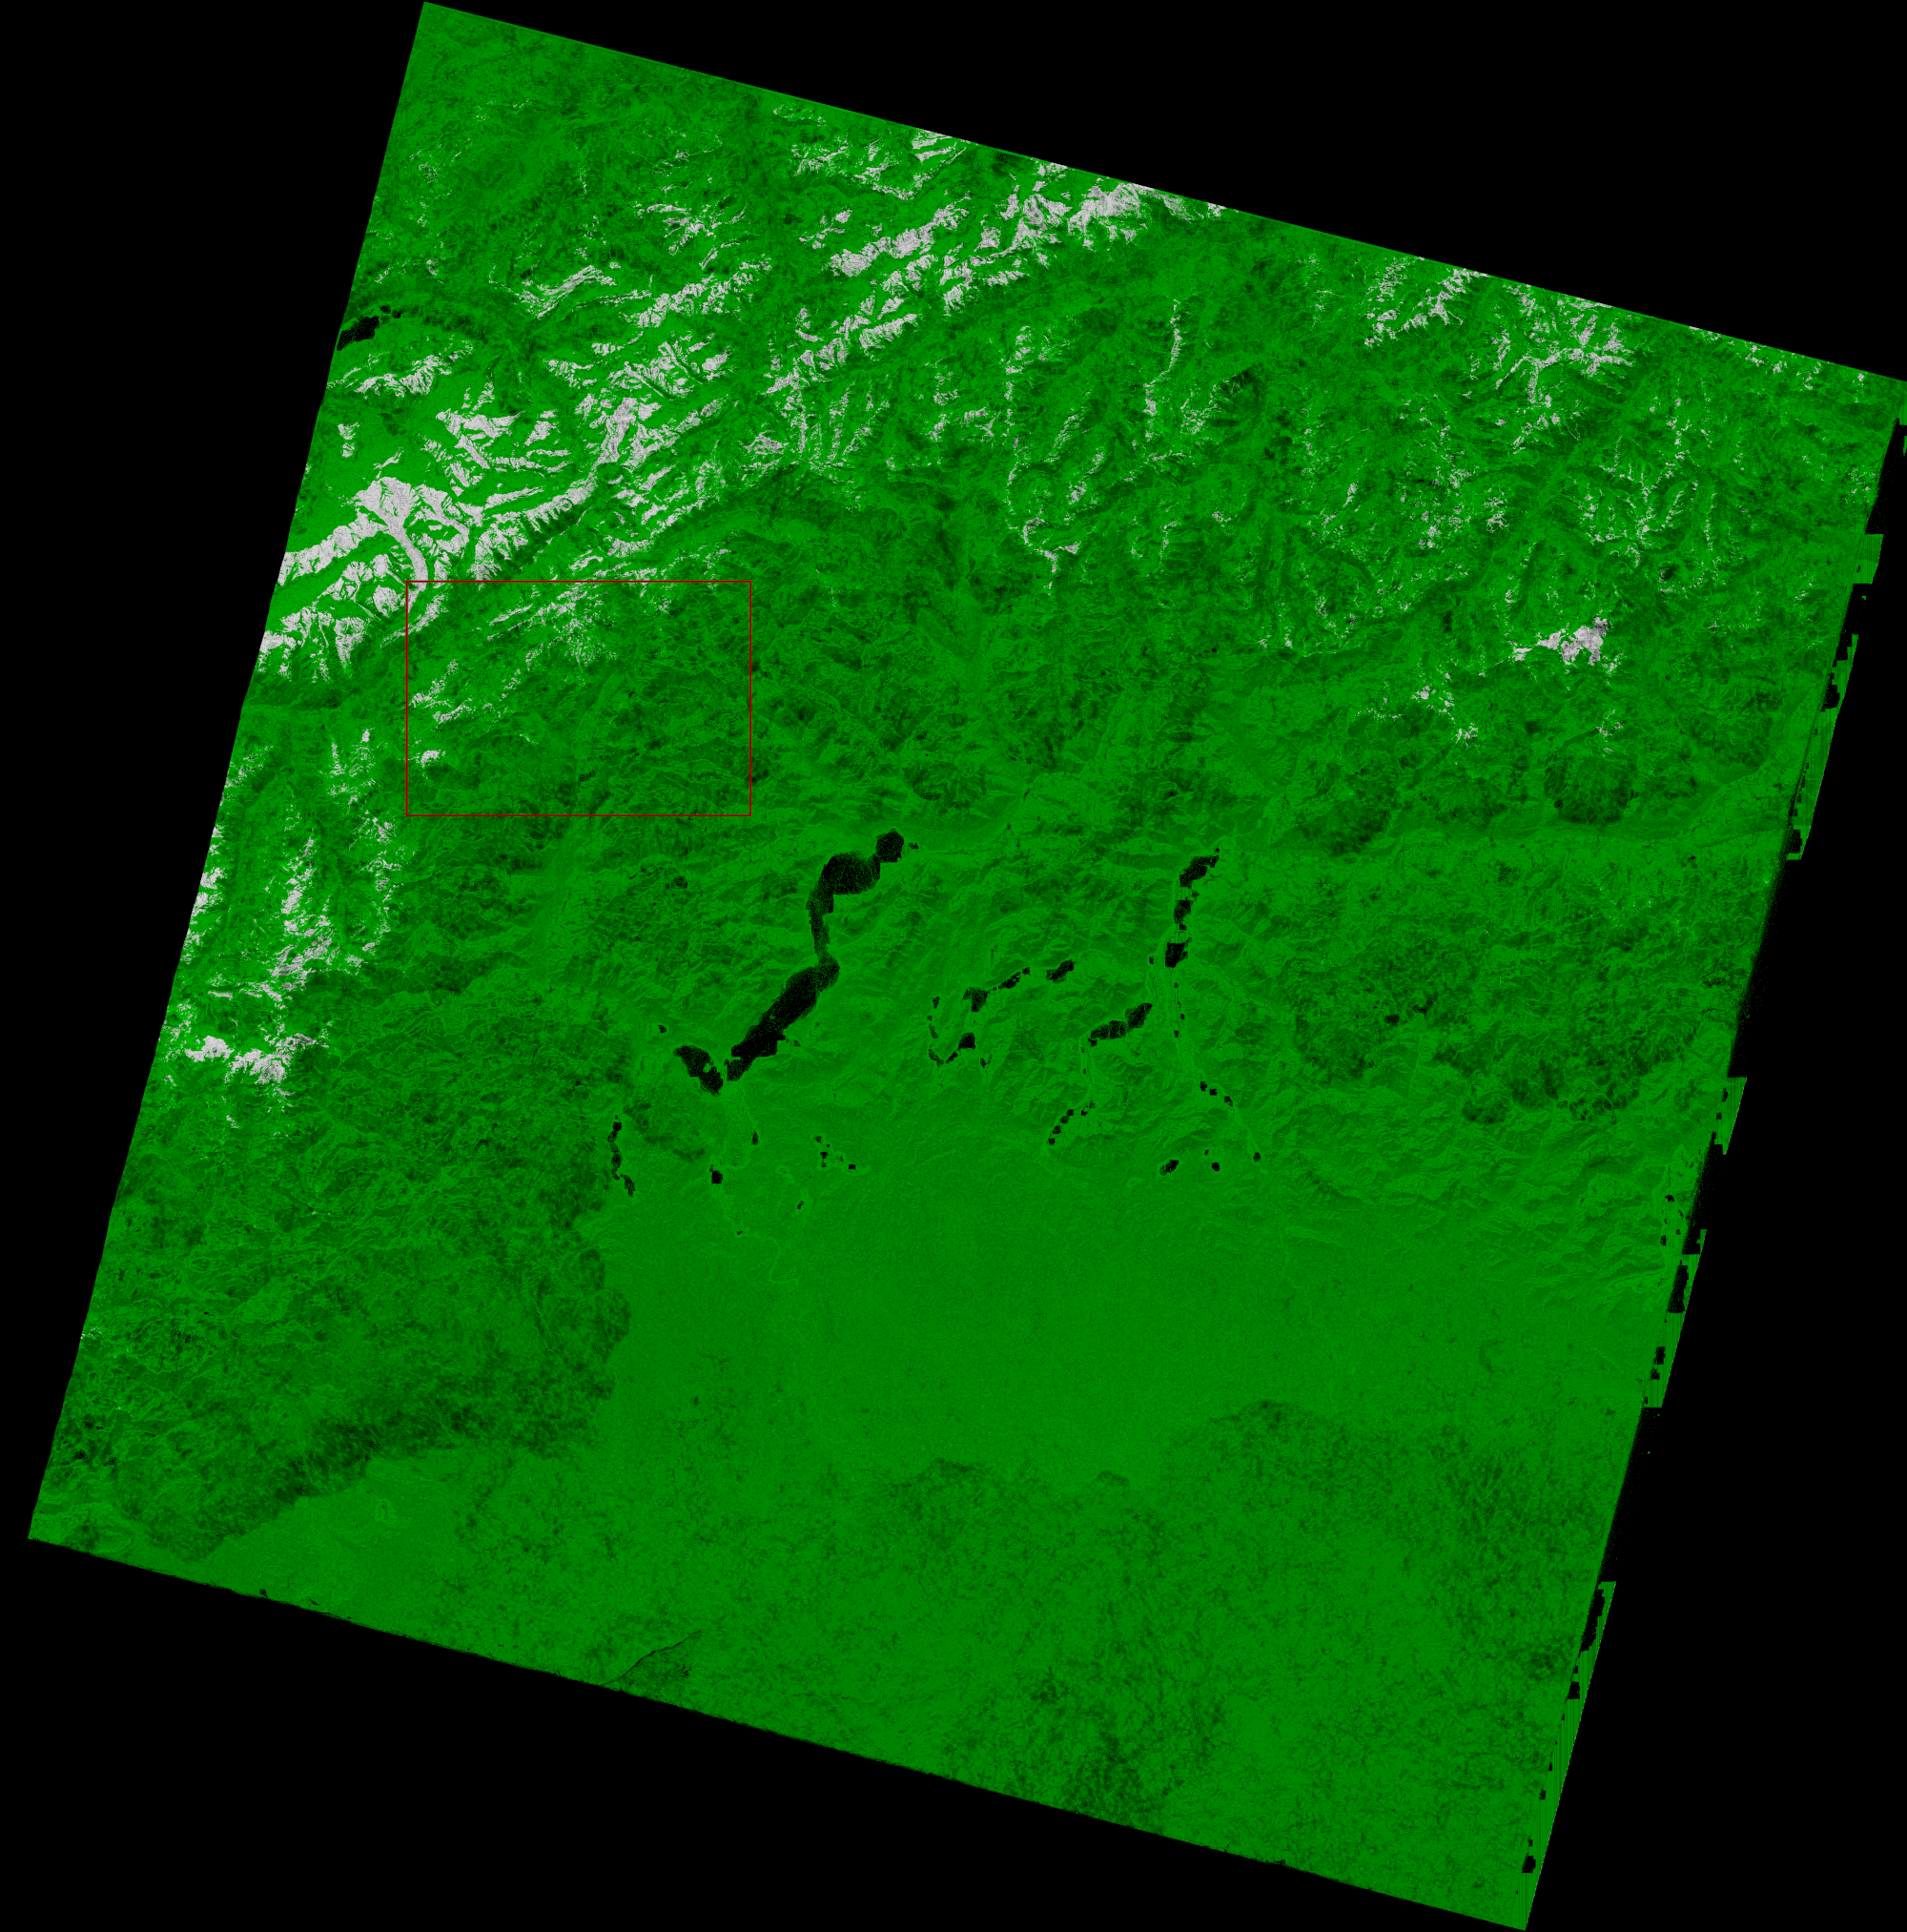
\includegraphics[width=\linewidth]{../images/LC81940282015363LGN02_Motion Predicted NDSI_unfiltered.png}
		\end{minipage}
		\begin{minipage}{0.45\textwidth}
			\centering
			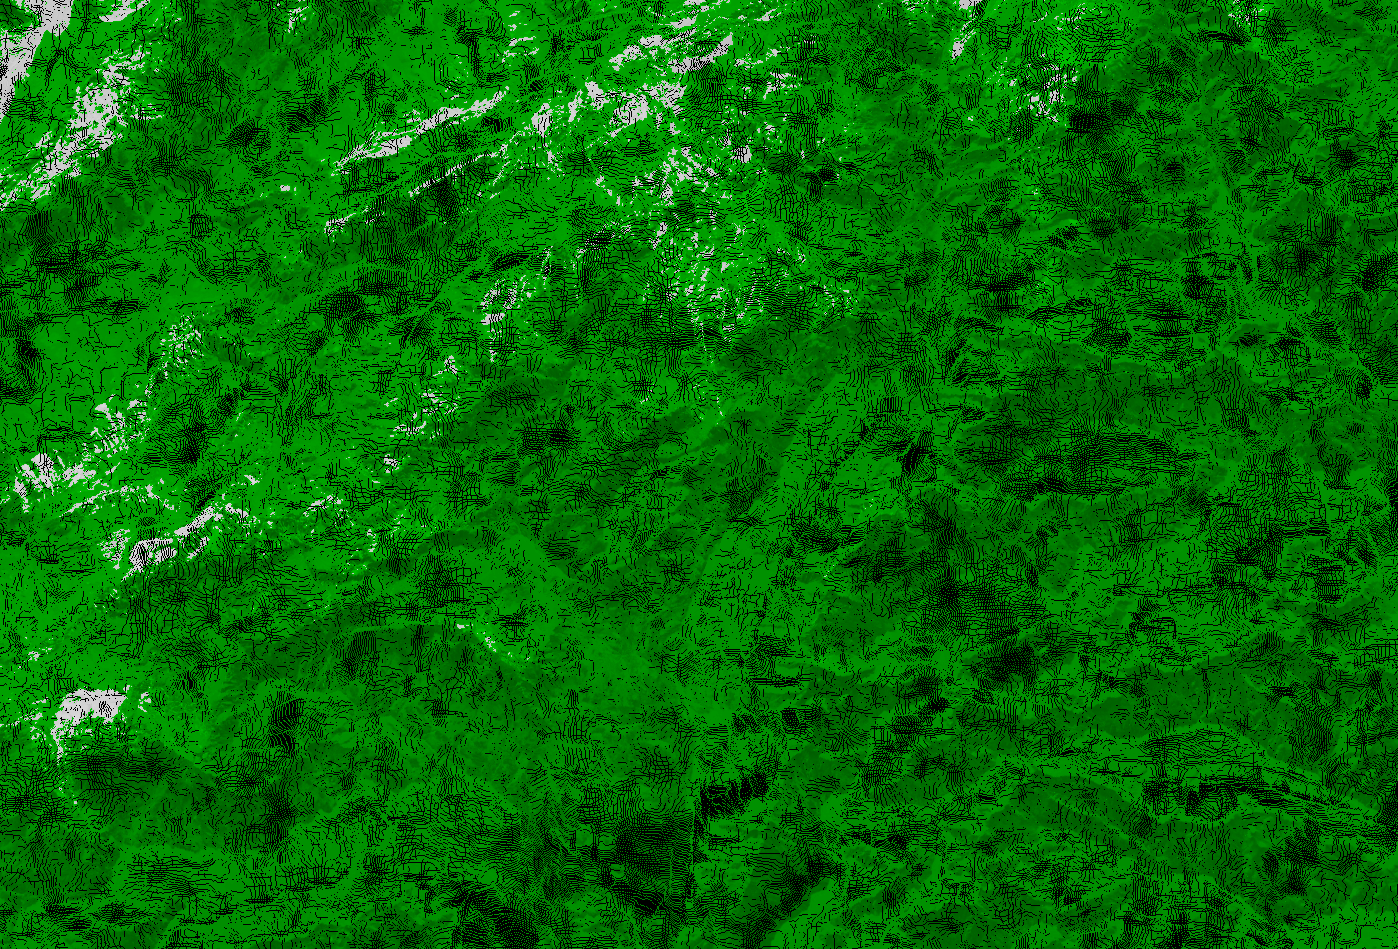
\includegraphics[width=\linewidth]{../images/LC81940282015363LGN02_Motion Predicted NDSI_unfiltered_small.png}
		\end{minipage}
		\caption{}
		\label{fig:unfiltered}
	\end{figure}

	\begin{figure}[h!]
	\centering
	\begin{minipage}{0.44\textwidth}
		\centering
		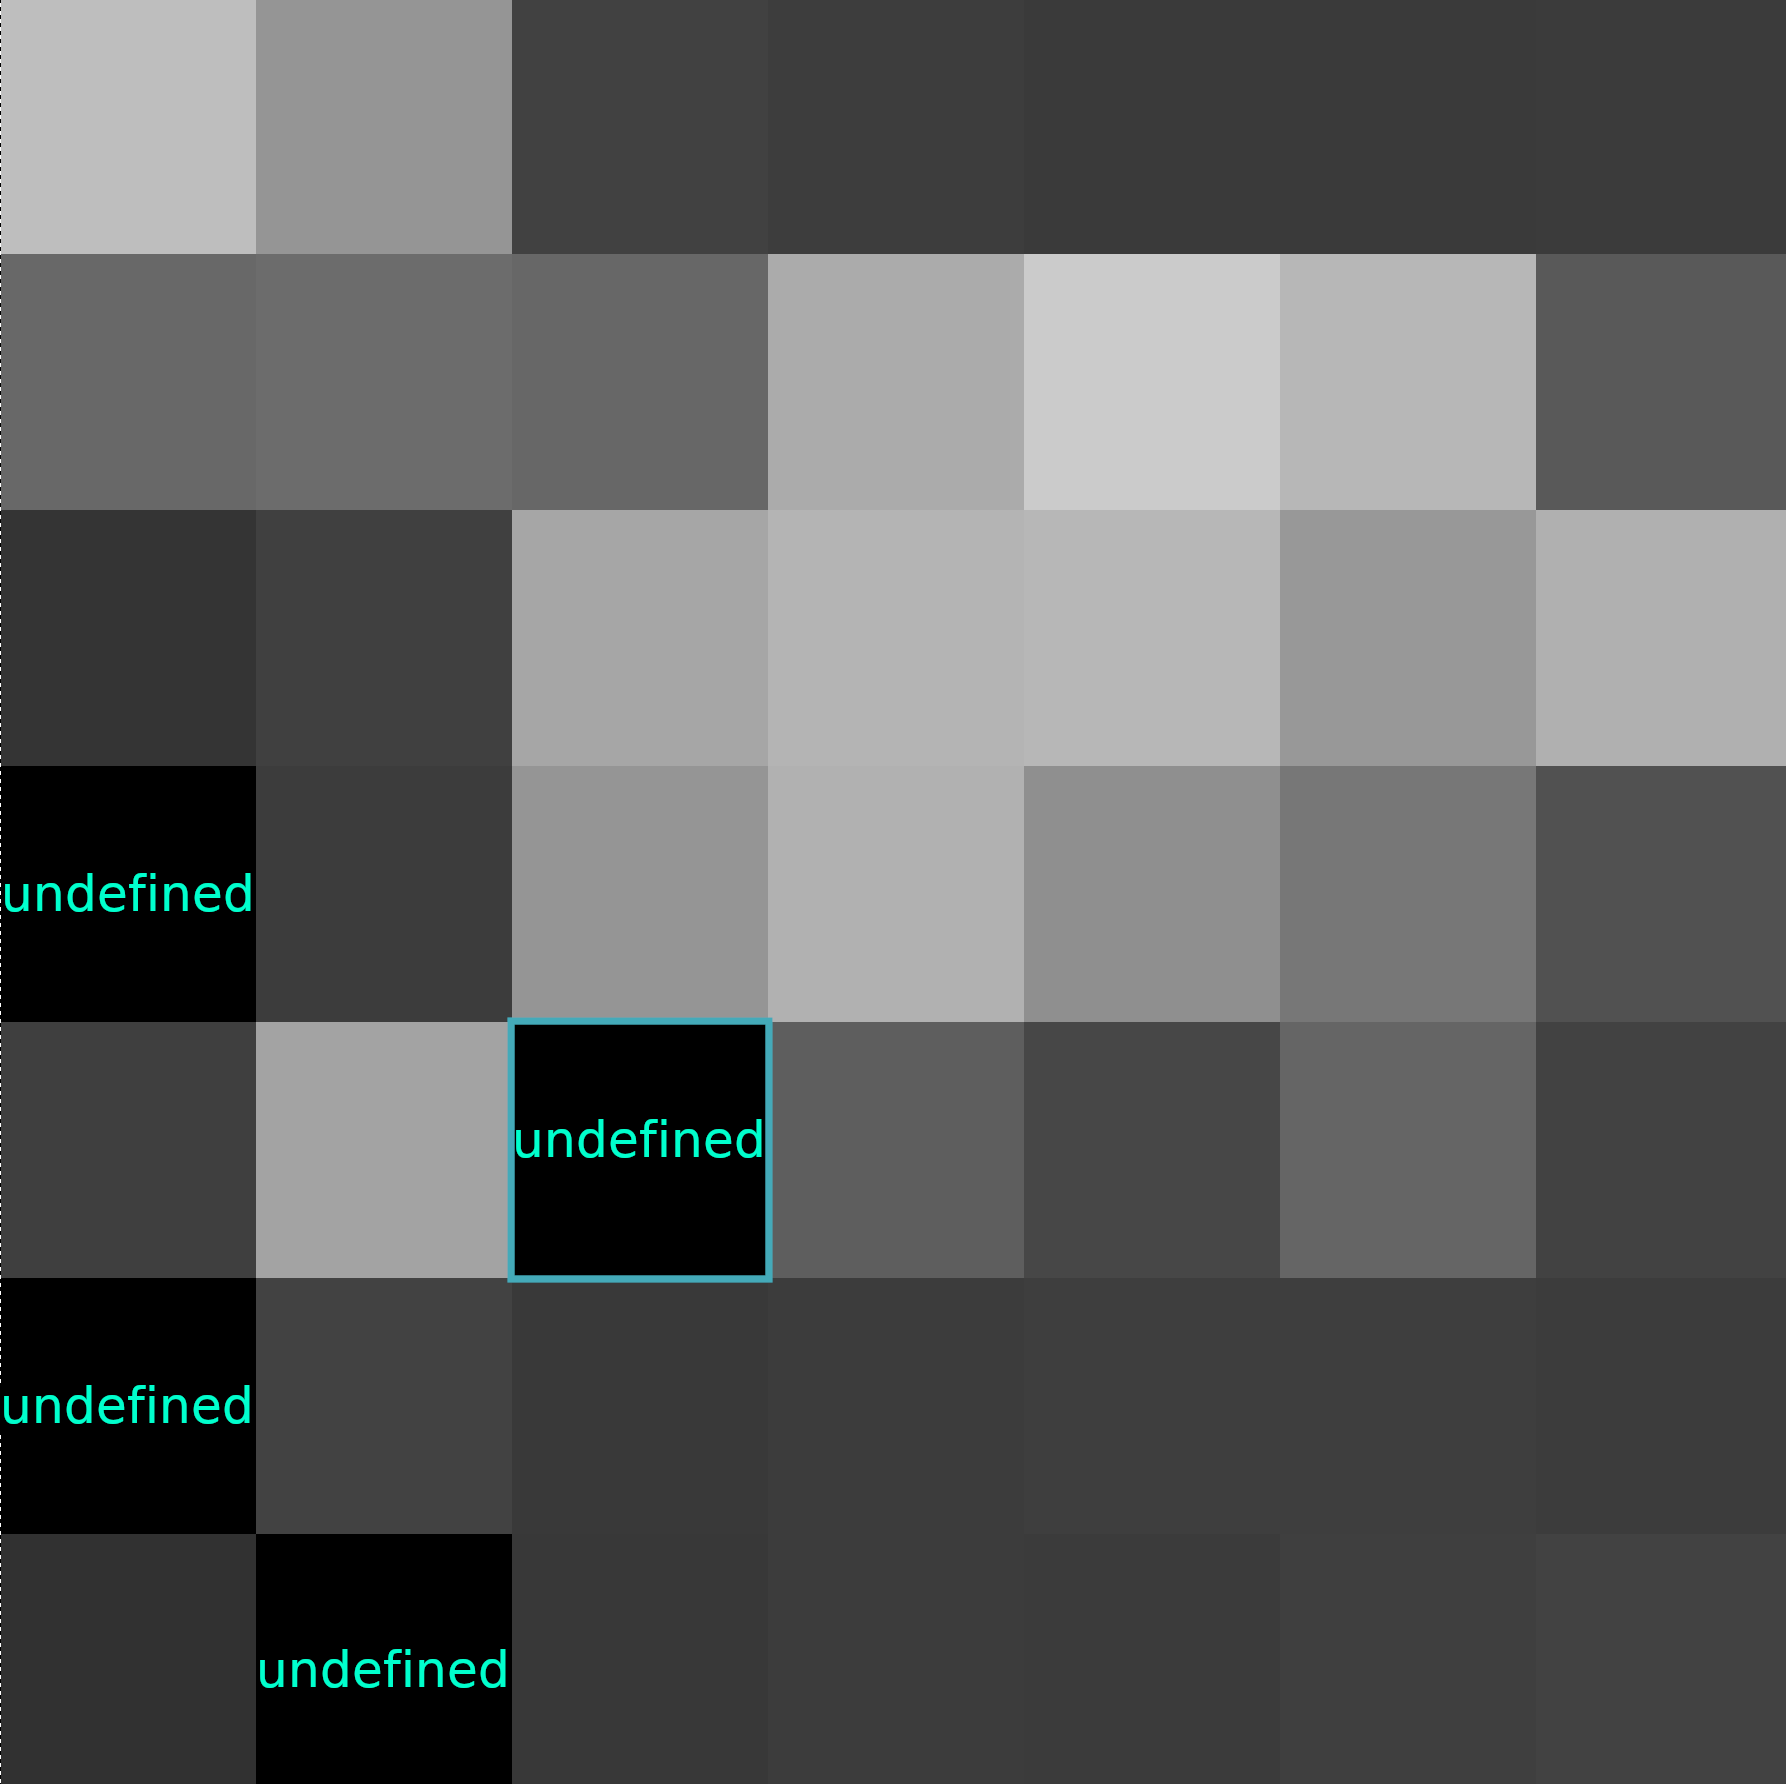
\includegraphics[width=\linewidth]{../images/gaussian_image.png}
	\end{minipage}
	\begin{minipage}{0.44\textwidth}
		\centering
		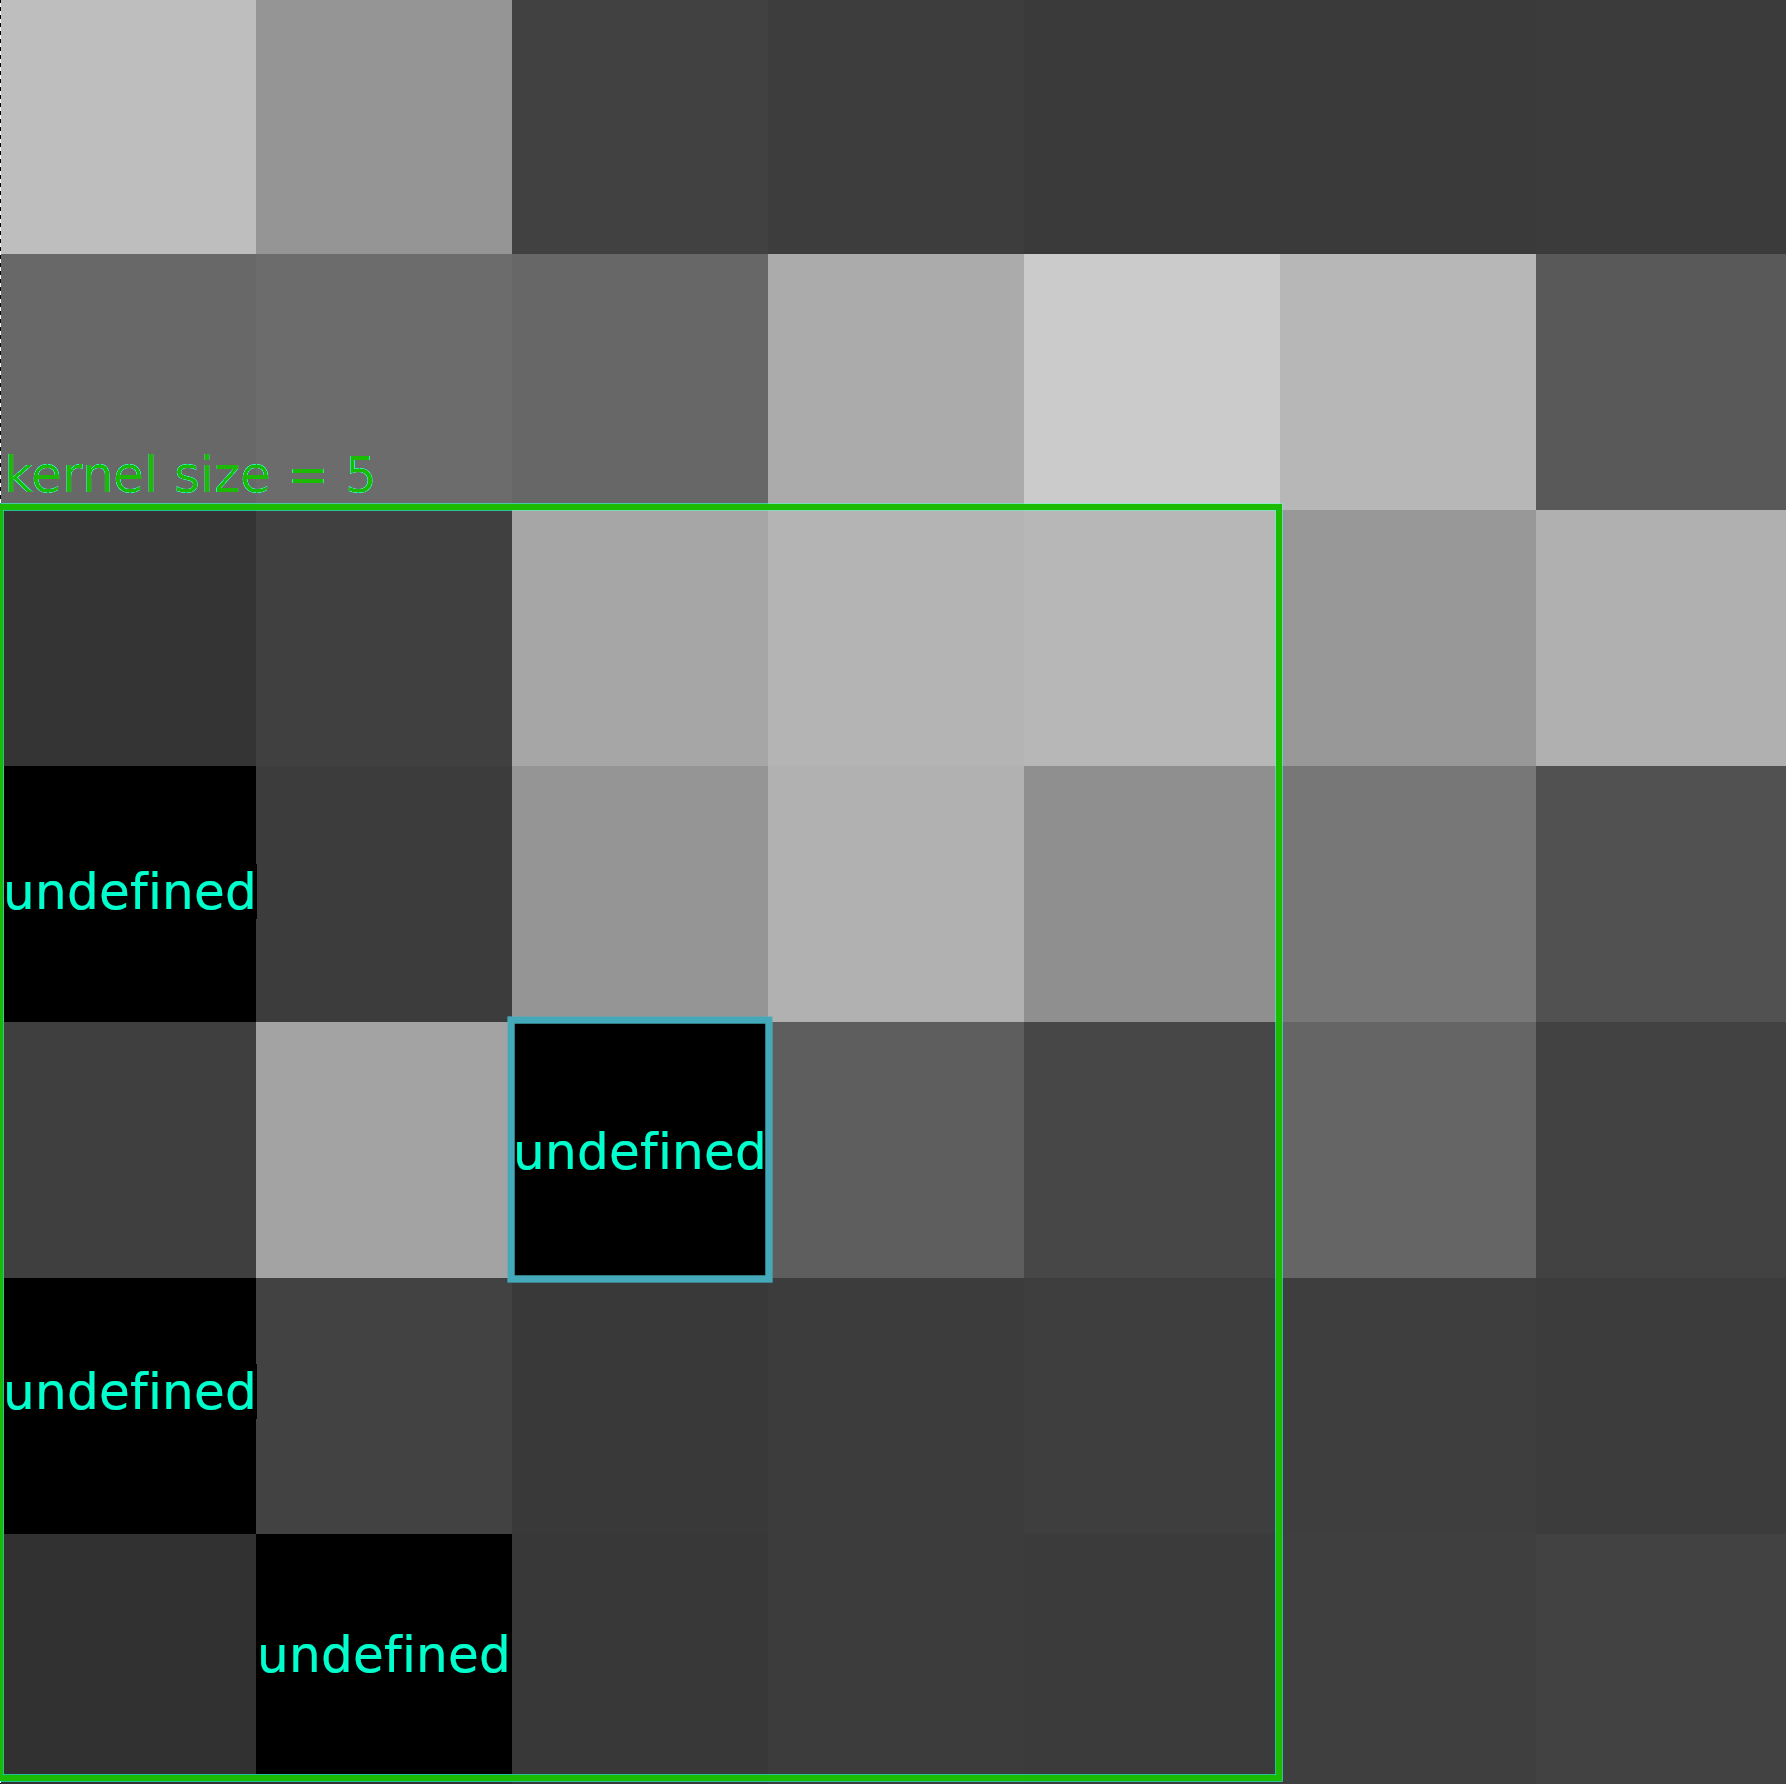
\includegraphics[width=\linewidth]{../images/gaussian_kernel1.png}
	\end{minipage}
	\begin{minipage}{0.44\textwidth}
		\centering
		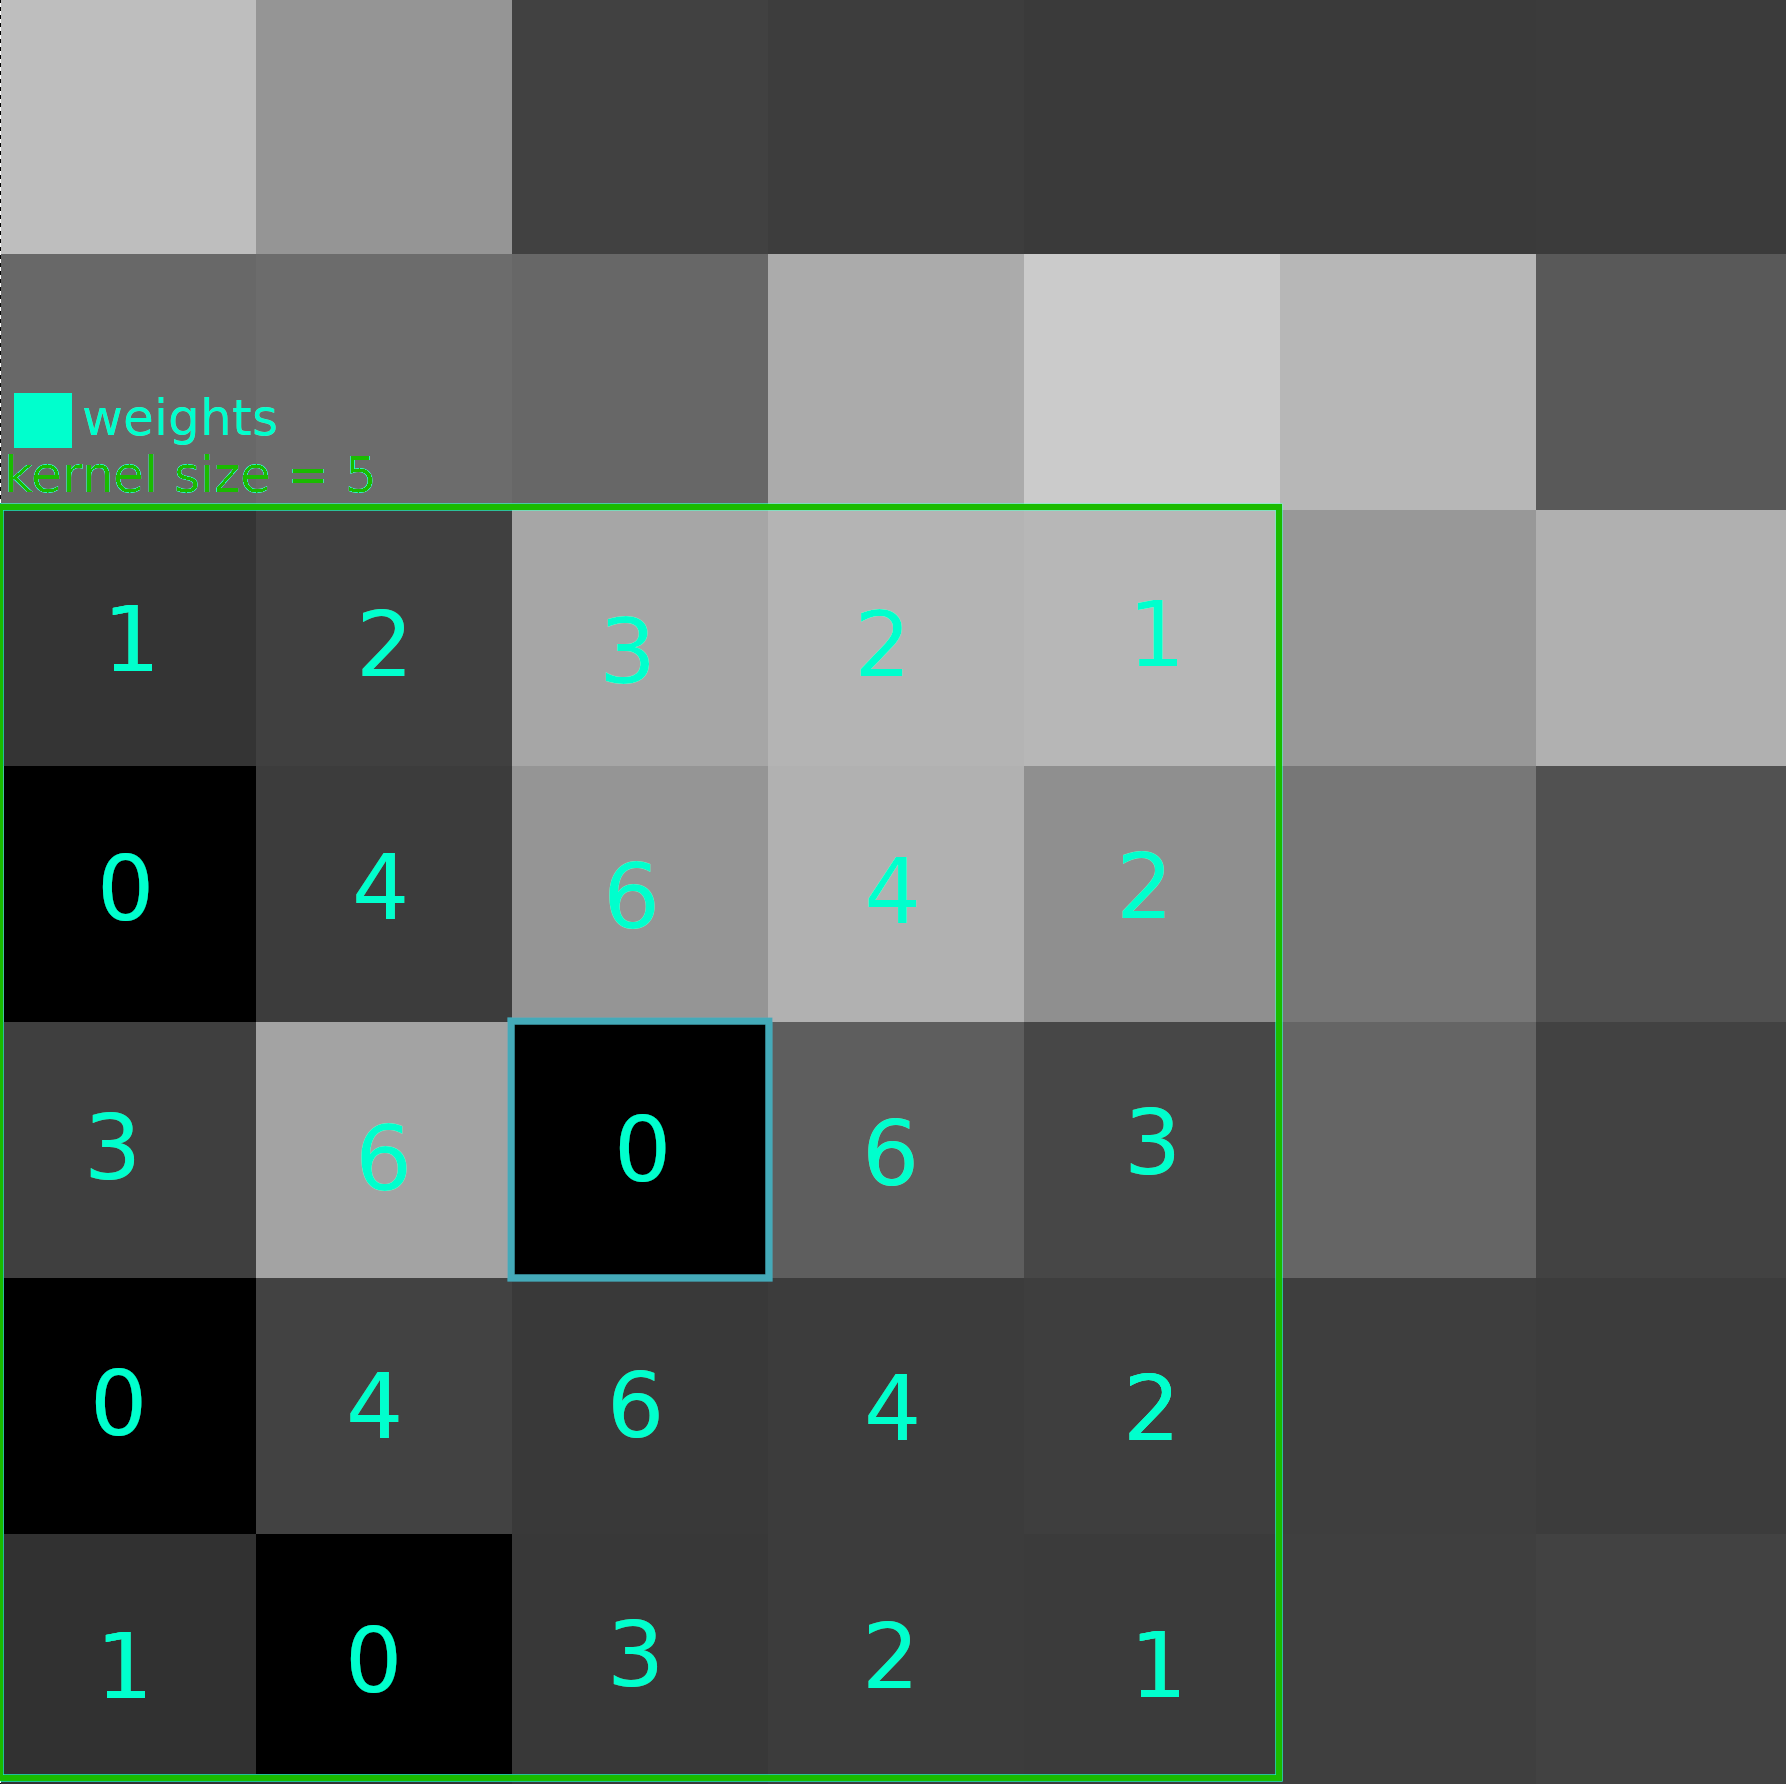
\includegraphics[width=\linewidth]{../images/gaussian_weights.png}
	\end{minipage}
	\begin{minipage}{0.44\textwidth}
		\centering
		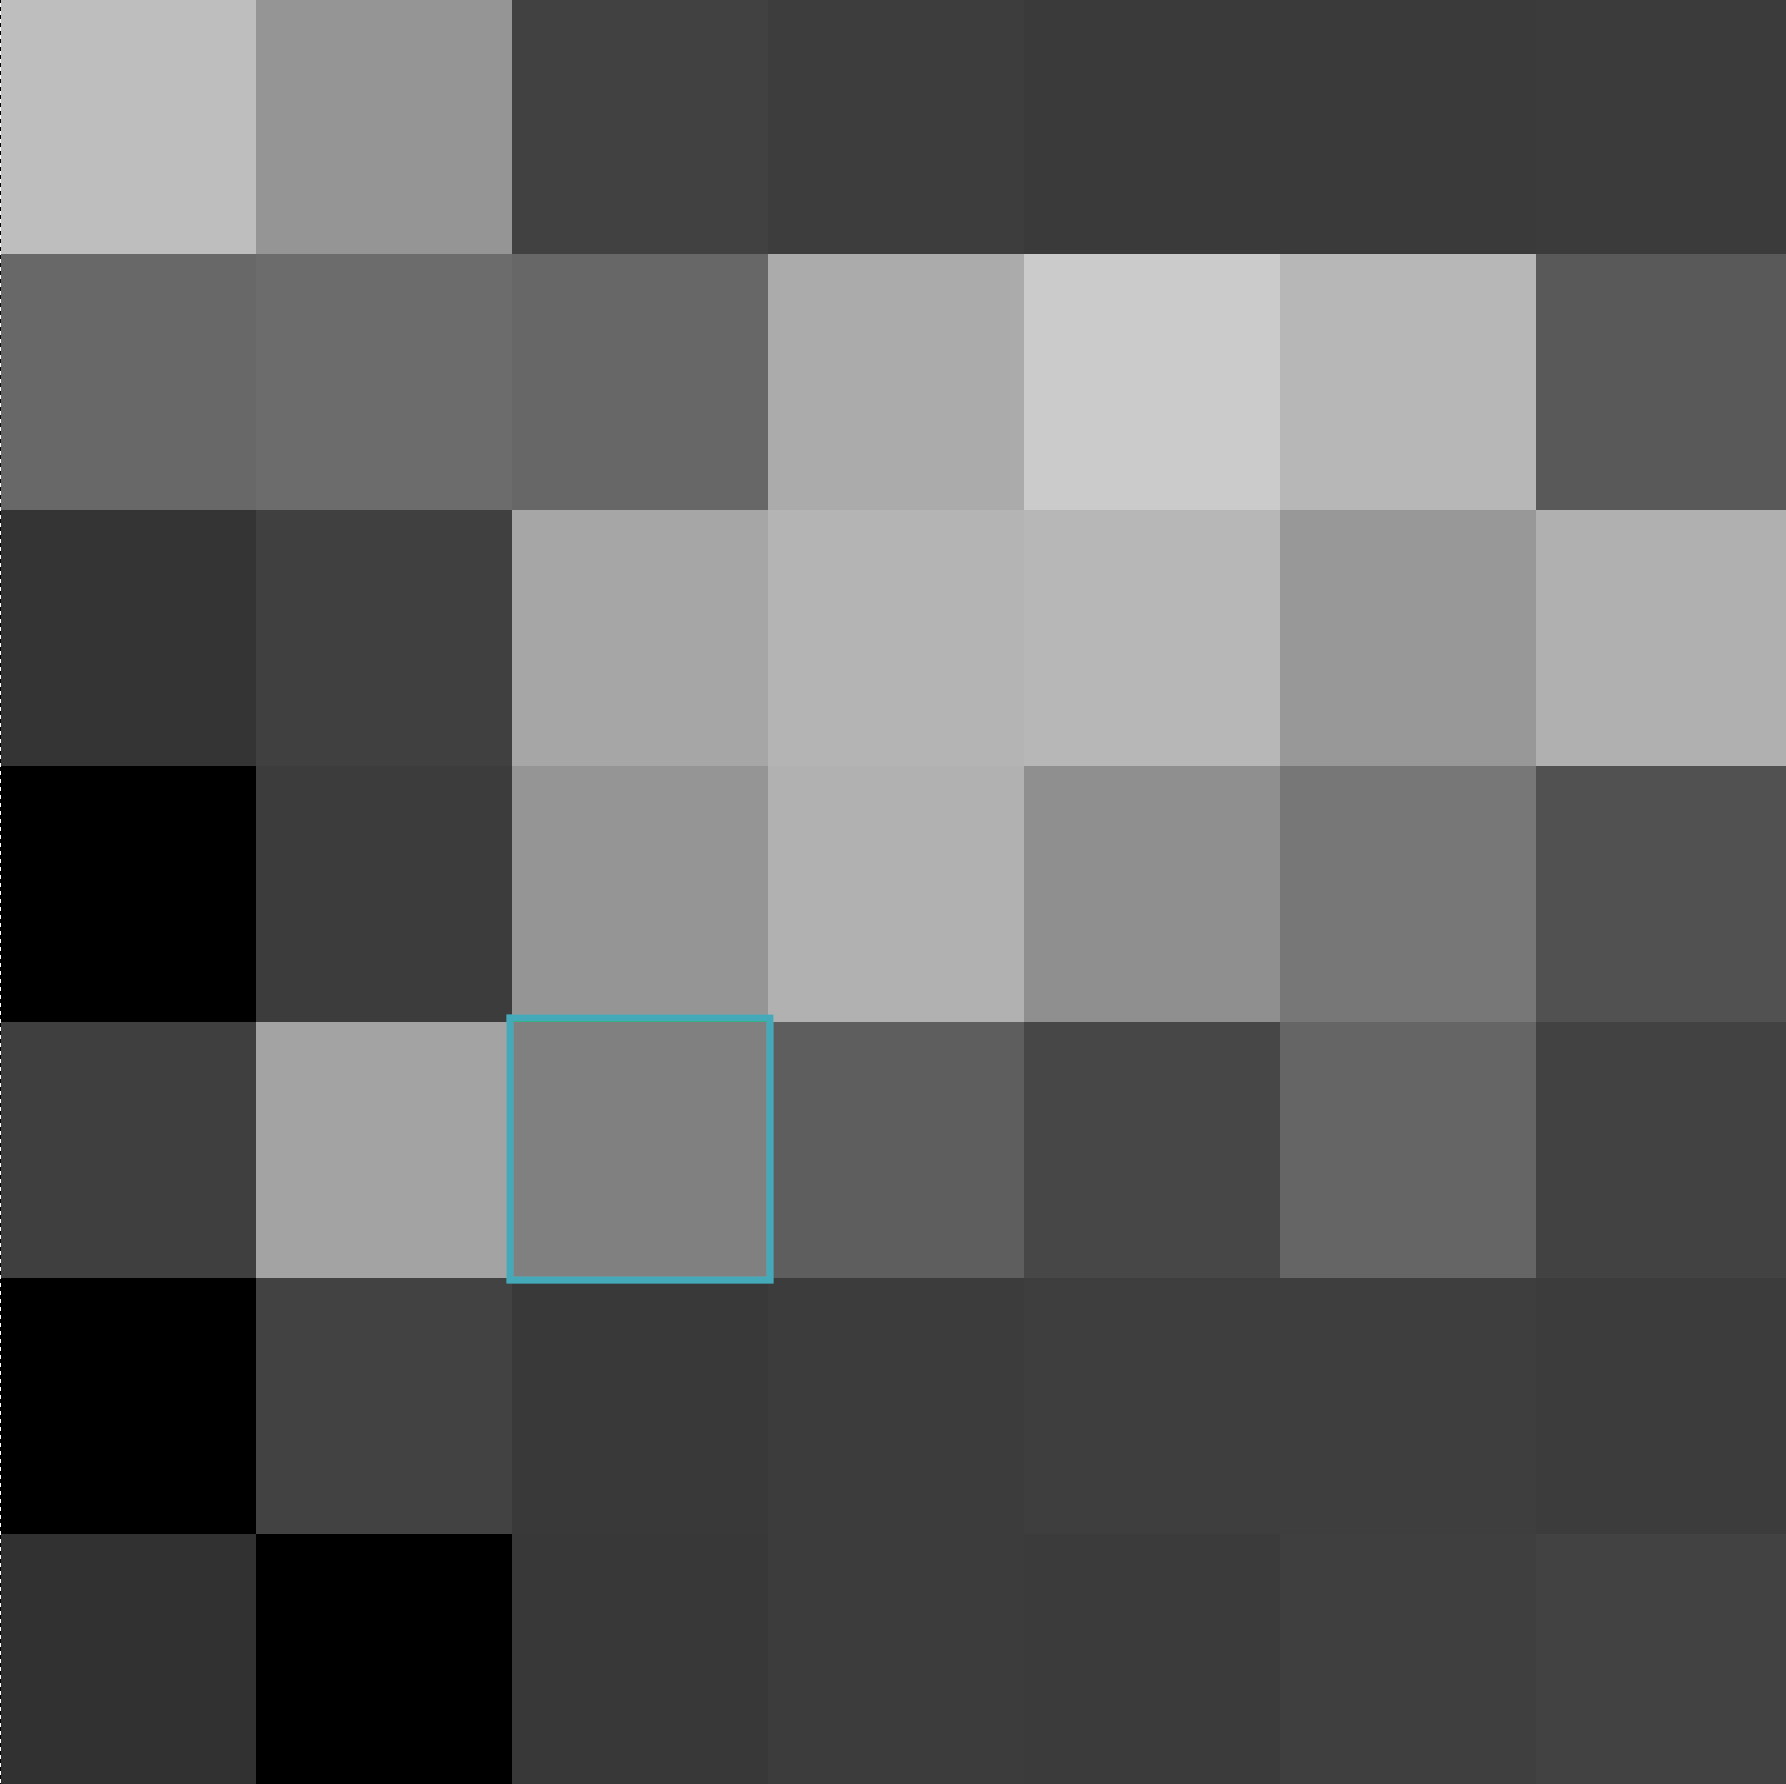
\includegraphics[width=\linewidth]{../images/gaussian_pixel.png}
	\end{minipage}
	\caption{Zoomed in part of the predicted NDSI (left, top). Neighbourhood extracted (right, top). Kernel of weights (left, bottom). Generated value (right, bottom).}
	\label{fig:gaussian}
	\end{figure}
	
	\par A first step into creating the filter for the motion predicted NDSI image is to create a \textbf{mask} which will be applied on the black border of the scene such that we are looking for \textbf{undefined values} only inside it. Using numpy, the \textbf{coordinates} of these pixels are extracted into an array which then can be processed in parallel by Pythons' \textbf{multiprocessing} library. We have used multiprocessing instead of threading because Python does not have true parallelization in multithreading, only concurrency, which would not be a real improvement on the processing time. Since all the processes have to write different chunks of the same image and they do not share the same memory space, we chose to solve this problem by creating a shared memory buffer to hold the image.

	\par The value of each found undefined pixel has to be calculated as an \textbf{weighted average} composed of its \textbf{neighbouring pixels}, as shown in Figure~\ref{fig:gaussian} top. We created the \textbf{kernel} which holds the weight of each pixel in the neighbourhood such that pixels closer to the centre have a higher weights than those near the edge. However, we have the case when we have multiple undefined pixels in the same neighbourhood. Since we cannot take their values in consideration, we do not want to include them in the weighted average, thus we set their weight to be 0, as shown in Figure~\ref{fig:gaussian} left, bottom. The result of the weighted average will be then stored as the value of the currently focused undefined pixel, as highlighted in Figure~\ref{fig:gaussian} right, bottom.

	% ===================================================================================
		
	\section{Extras}
	\label{seq:extras}
	Below we will talk about the 

	
	\subsection{Programming environment}
	\label{seq:programmingenv}
	
	\par The application part of the thesis has been written with the help of the \textbf{Emacs} text editor, mainly because it provides a uniformity which supports various working flows, since it is not focused on a specific programming language, like PyCharm or Eclipse, for example. The editor is highly customizable and it provides structured, powerful commands for text editing, file searching, in-place code versioning and many more.
	
	\subsection{Programming language}
	\label{seq:programminglang}
	
	\par For the purpose of the thesis we have used the \textbf{Python} programming language mainly because of its numerous available libraries which support computer vision, heavy mathematical computations and raster image processing. The most important libraries used in this application are listed at Section~\ref{seq:libraries}.
	
	\subsection{Libraries}
	\label{seq:libraries}
	
	\subsubsection{NumPy}
	
	\par Since the data used for this thesis is large in size, relying on Python alone for data structures for processing does not scale. Python is an interpreted language, not a compiled one, which means that for each operation its interpreter has to do extra work such that it translated the bytecode instruction into a form that is machine executable. For a large number of operation, such as we have high resolution images, this does not scale. Instead, we resorted to using NumPy, which is an open-source library which brings support of large data computation, such as multi-dimensional arrays and matrices, as well as a large collection of mathematical functions which can be easily used for their operation \cite{arraynumpy}. The library has a \textbf{well optimised C code core} which can handle large processing by bypassing the python interpreter, which results in the speed of a compiled language, not an interpreted one. Therefore, based on the needs of our dataset, we have used NumPys' main data structure, the ndarray (n-dimensional array) as a data structure to hold our images and various optimisations applied throughout processing focused on using only this type of data structure in order to make use of NumPys' optimisations and speed.
	
	\subsubsection{Open Source Computer Vision Library (OpenCV)}
	
	\par The OpenCV library brings support for \textbf{computer vision processing}, by providing programming functions which can be reliably used \cite{cuda}. Its use in our thesis both for image alignment and detecting motion through deep optical flow, by using its already integrated functions as a support. OpenCV, as well as NumPy, is open-source and it is written and optimised in native code, which is needed for the large size of our dataset entities.
	
	\subsubsection{Geospatial Data Abstraction Library (GDAL)}
	
	\par The GDAL library is a translator for vector and \textbf{raster geo-spatial data formats}, which presents a single data model to work with \cite{gdal}. Since our images are represented in the tiff format, reading them by using GDAL proved to be the easy and reliable.
	
	\subsubsection{Version-control}
	\label{seq:versioning}
	
	\par In order to keep track of various changes, bugs and enhancements of our application, we had to make sure that we are using a \textbf{reliable version-control} system. For this purpose, Git was chosen for its fast performance with the aim of data integrity and support for distributed workflows \cite{git}. When a directory is flagged as a git repository, it keeps track of any changes made to that location, independent of a central server of network accessibility. By keeping a clean workflow, one can easily include enhancements and try experiments without the worry of losing stability. We have kept track of every change, bug and enhancement from the beginning of developing this application by using git, and the repository which contains all of this information can be found on Github, at \textbf{\url{https://github.com/BabyCakes13/GlacierImagePredictor}}.
	
	\newpage{}
	\chapter{Performance and experiments}
	\label{seq:performance}
	
	\par To exemplify the functionality of our application, we have picked two glaciers and downloaded all their public available satellite imagery with at most 20\% cloud coverage. 
	
	\par The first glacier which will be analysed is named \textbf{Jungfrau-Aletsch-Bietschhorn}, located in the \textbf{Swiss Alps}, specifically at latitude 46.47735081308319 and longitude 8.056887228860798. This location is at the intersection of multiple WRS-2 coordinates, therefore we will have multiple sets of \(path, row, month\) which we will be focusing on.
	
	\subsection{Jungfrau-Aletsch-Bietschhorn (194, 28, 4)}
	
	\begin{figure}[h!]
		\centering
		\begin{minipage}{0.5\textwidth}
			\centering
			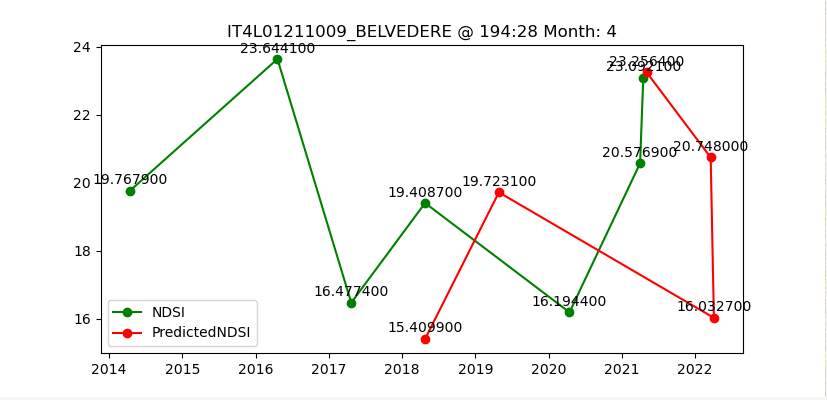
\includegraphics[width=\linewidth]{../images/experiment_194284.png}
		\end{minipage}
		\caption{Comparison between the NDSI values of the actual NDSI images for Jungfrau-Aletsch-Bietschhorn(194, 28, 4), and the NDSI of each predicted motion image.}
		\label{fig:jungfrau_194284}
	\end{figure}
	
	\begin{figure}[h!]
		\centering
		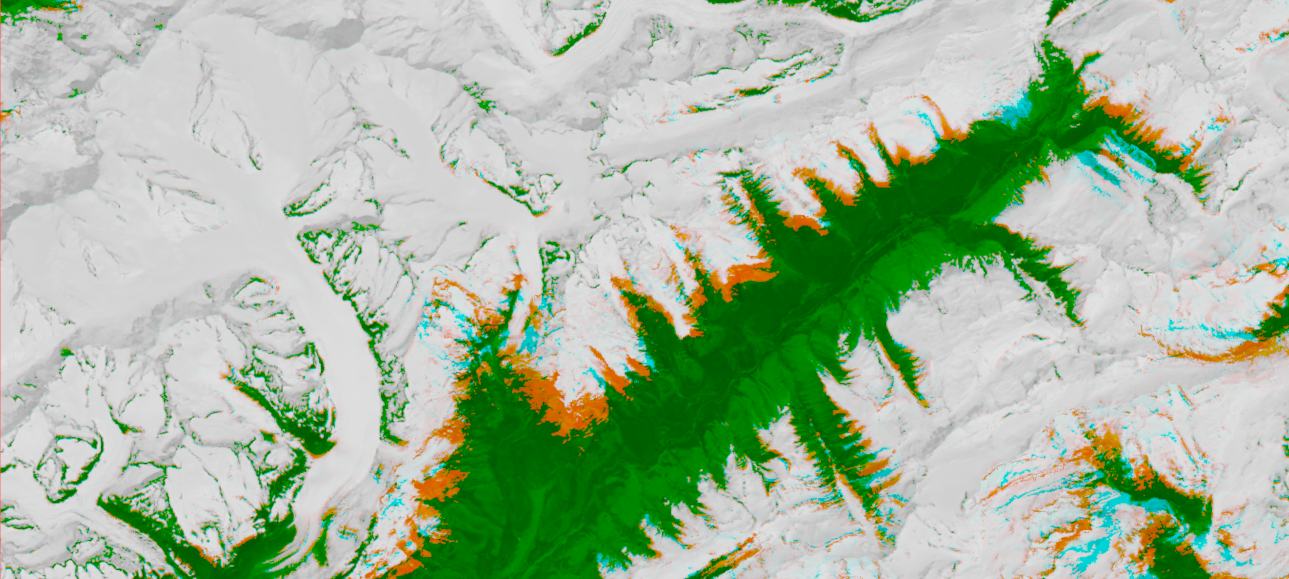
\includegraphics[width=\linewidth]{../images/experiment_1940284_image.png}
		\caption{Overlapped motion generated NDSI for scene LC81940282017112LGN00.}
		\label{fig:experiment_1940284_image}
	\end{figure}

	% =================================================================
	
	\subsection{Jungfrau-Aletsch-Bietschhorn (194, 28, 7)}
	
	\begin{figure}[h!]
		\centering
		\begin{minipage}{0.44\textwidth}
			\centering
			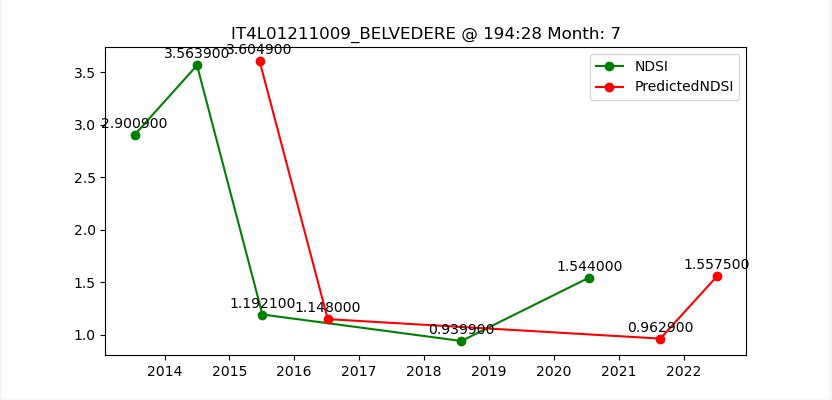
\includegraphics[width=\linewidth]{../images/experiment_194287.png}
		\end{minipage}
		\caption{Comparison between the NDSI values of the actual NDSI images for Jungfrau-Aletsch-Bietschhorn(194, 28, 7), and the NDSI of each predicted motion image.}
		\label{fig:jungfrau_194287}
	\end{figure}
	
	\begin{figure}[h!]
		\centering
		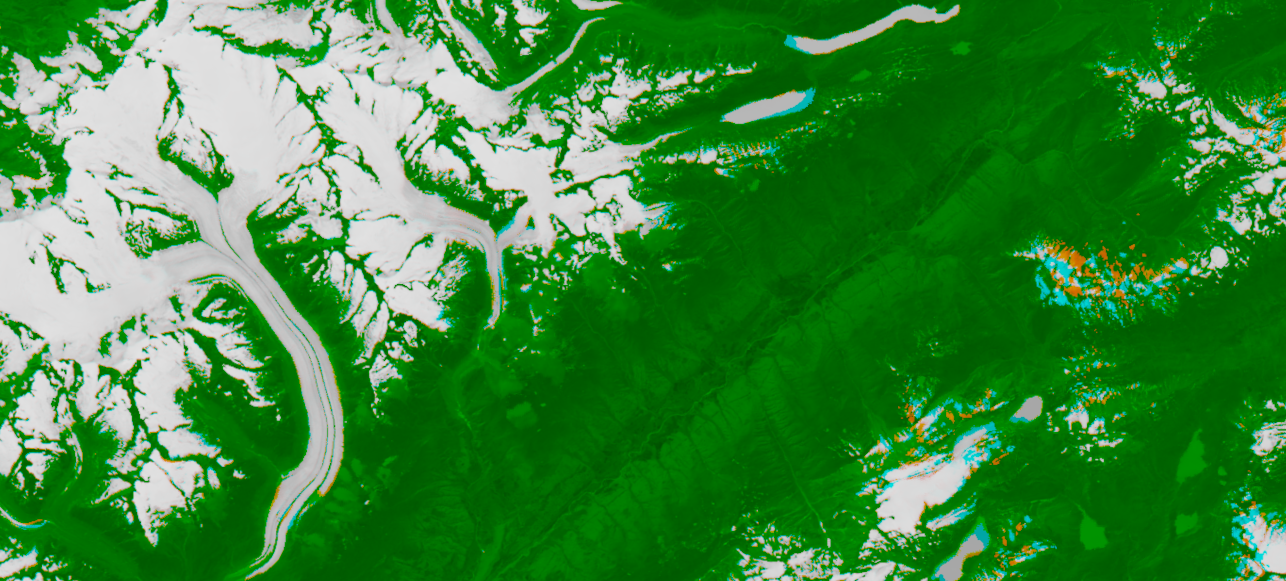
\includegraphics[width=\linewidth]{../images/experiment_1940287_image.png}
		\caption{Overlapped motion generated NDSI for scene LC81940282020201.}
		\label{fig:experiment_1940287_image}
	\end{figure}

	% ===================================================================
	
	\subsection{Jungfrau-Aletsch-Bietschhorn (194, 28, 8)}
	
	\begin{figure}[h!]
		\centering
		\begin{minipage}{0.44\textwidth}
			\centering
			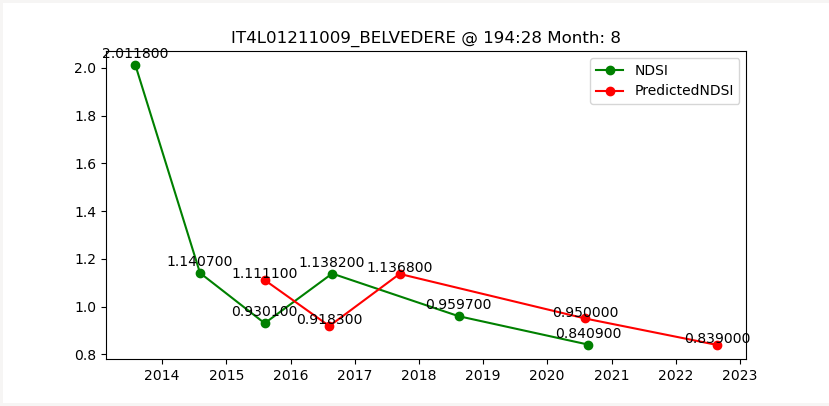
\includegraphics[width=\linewidth]{../images/experiment_194288.png}
		\end{minipage}
		\caption{Comparison between the NDSI values of the actual NDSI images for Jungfrau-Aletsch-Bietschhorn(194, 28, 7), and the NDSI of each predicted motion image.}
		\label{fig:jungfrau_194288}
	\end{figure}
	
	\begin{figure}[h!]
		\centering
		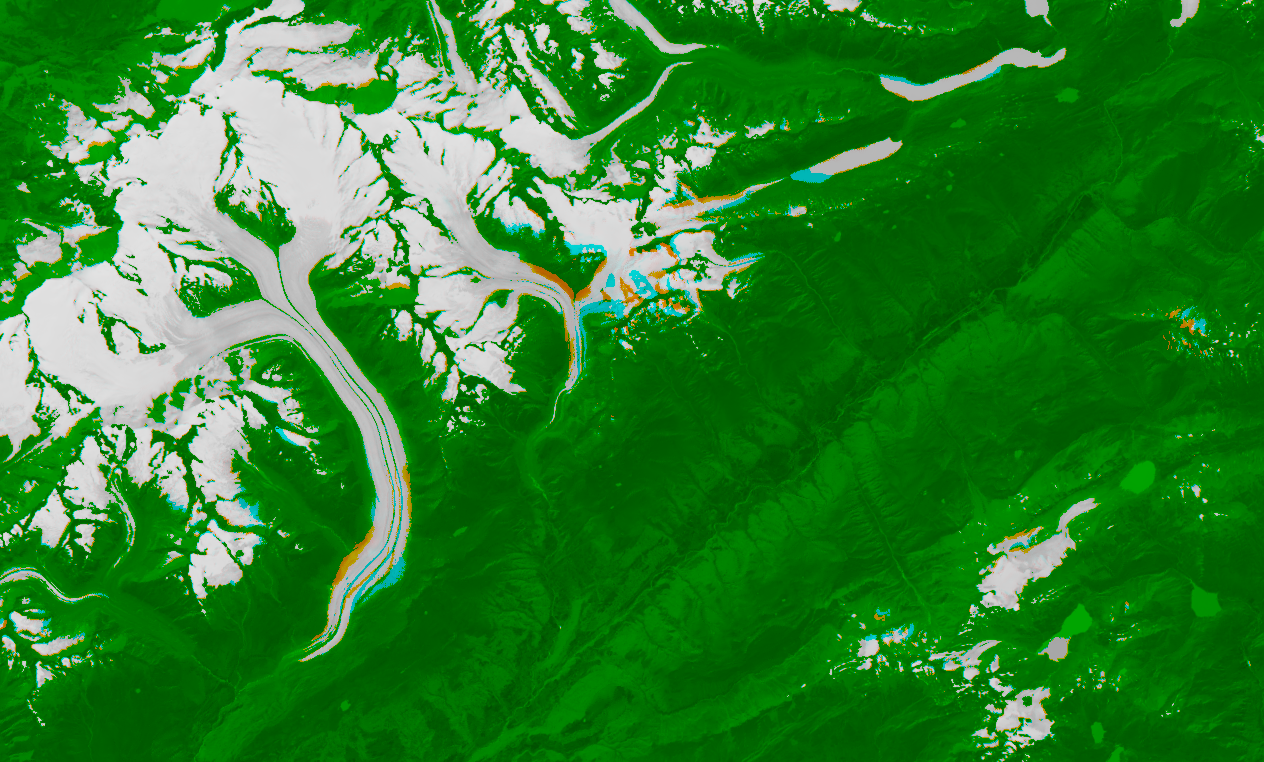
\includegraphics[width=\linewidth]{../images/experiment_1940288_image.png}
		\caption{Overlapped motion generated NDSI for scene LC81940282016238LGN01.}
		\label{fig:experiment_1940288_image}
	\end{figure}
	
	% ==================================================================
	
	\subsection{Jungfrau-Aletsch-Bietschhorn (195, 28, 9)}
	
	\begin{figure}[h!]
		\centering
		\begin{minipage}{0.44\textwidth}
			\centering
			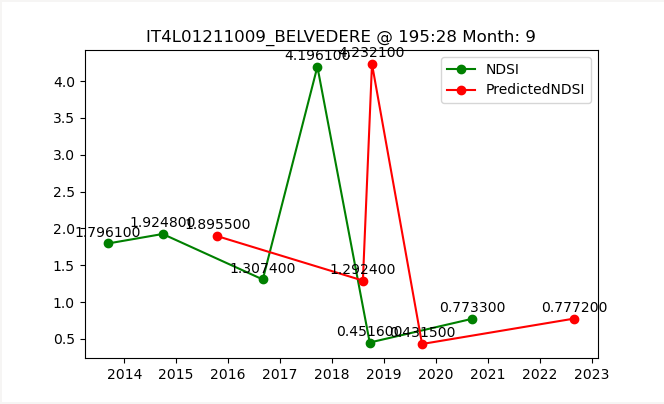
\includegraphics[width=\linewidth]{../images/experiment_195289.png}
		\end{minipage}
		\caption{Comparison between the NDSI values of the actual NDSI images for Jungfrau-Aletsch-Bietschhorn(195, 28, 9), and the NDSI of each predicted motion image.}
		\label{fig:jungfrau_195289}
	\end{figure}

	\begin{figure}[h!]
	\centering
	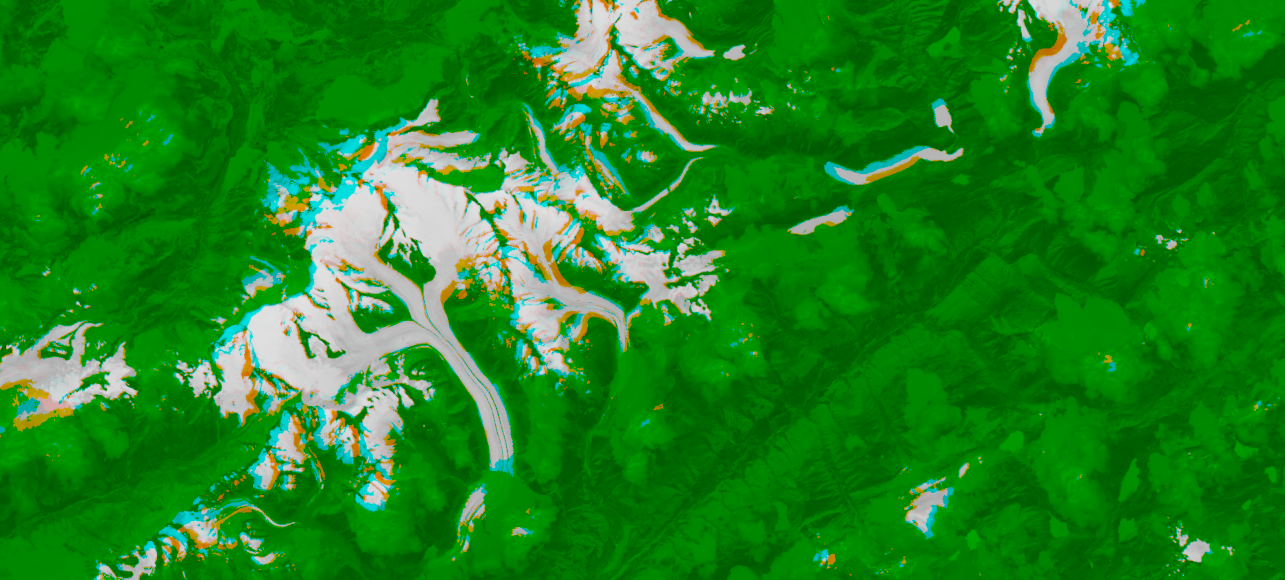
\includegraphics[width=\linewidth]{../images/experiment_1950289.png}
	\caption{Overlapped motion generated NDSI for scene LC81950282020256.}
	\label{fig:experiment_1950289_image}
	\end{figure}
	
	\par The second glacier which we have taken into consideration is named \textbf{Parvati} and it is located in \textbf{India}, at latitude 31.754 and longitude 77.675. We have chosen this glacier such that we can compare our results with the ones provided in \cite{parvati}. They have chosen a dataset of images located at WRS-2 path 147, row 38. However, we could not fetch enough quality images for that specific path and row in order to be able to make this comparison. The result that were achieved are however listed below for the available path and row.
	
	\subsection{PARVATI (146, 38, 4)}
	
	\begin{figure}[h!]
		\centering
		\begin{minipage}{0.44\textwidth}
			\centering
			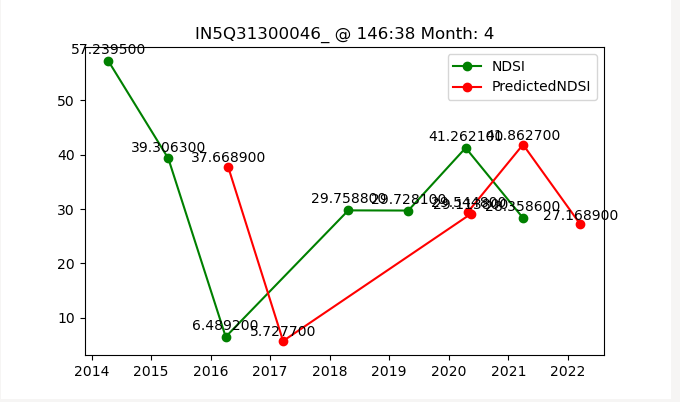
\includegraphics[width=\linewidth]{../images/experiment_146385.png}
		\end{minipage}
		\caption{Comparison between the NDSI values of the actual NDSI images for Parvati(146, 38, 4), and the NDSI of each predicted motion image.}
		\label{fig:parvati_146384}
	\end{figure}

	\begin{figure}[h!]
	\centering
	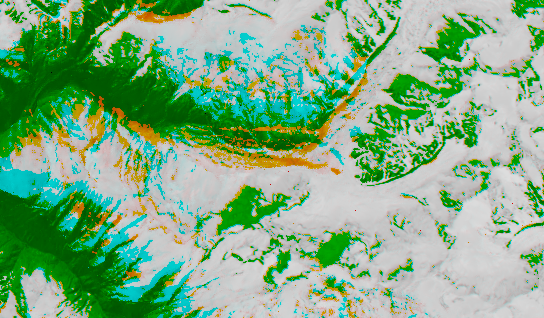
\includegraphics[width=\linewidth]{../images/experiment_1460384_image.png}
	\caption{Overlapped motion generated NDSI for scene LC81460382021091.}
	\label{fig:experiment_1460384_image}
	\end{figure}
	
	\begin{itemize}
		\item 
	\end{itemize}
	
	\par Here we should also write on what machine I ran the code and try it on different ones as a thing. Also write about the idea of moving the processing on cloud, but there might be traffic overhead because the images are large. Also say that we store it on hard drive, NOT ssd. Make tests with both.
	
	\newpage{}	
	\chapter{Conclusions}
	\label{seq:conclusions}
	
	\section{Future Development}
	\label{seq:future_development}
	
	\par During the process of creating the application, multiple \textbf{problems} were met. One of them was that even though there are a large number of aerial images collected in the collection provided for the Landsat 8 satellite, there are not many which have a small enough cloud coverage. This results in datasets with a low number of entities, which means that we cannot test our results on a longer period of time. Since clouds interfere with delimiting snow and pixels from a scene, if we wanted to broaden our dataset, we thought of two options:
	
	\begin{itemize}
		\item harvesting images from \textbf{multiple satellites}, such as Sentinel and older versions of Landsat. Even if these satellites use other types of sensors on board for Earth observation, by matching the wavelengths of their bands one could make a match between them. By using multiple satellites, more populated datasets can be created, since we are taking into consideration collected scenes over the years for pairs of paths, rows and months. By only using Landsat 8, even with an allowed cloud coverage of 20\%, the average length of a \(path, row, month\)) dataset was around 15;
		\item implementing \textbf{cloud mapping algorithms} such that cloud could be detected and trimmed out before the calculation of the normalized snow difference index and optical flow extraction. For now, the optical flow algorithm ran between scenes which have a high cloud coverage finds large vectors of motion at the locations where clouds existed from one frame to another. The result does not take into consideration the difference between snow pixels and cloud ones, therefore all of them are moved. 
	\end{itemize}

	\par Another improvement could be changing the way that the coordinates of the pixels of the motion generated image are calculated. For now, we are predicting their location by using the method described in \ref{fig:motion_generated_schema}, where we are multiplying by two both the original coordinates and the time. A more interesting approach would be using \textbf{time series forecasting models} applied on the distance vectors generated by optical flow for each pixel over time in order to generate future entries. This could be done with statistical methods such as the autoregressive integrated moving average (ARIMA). However, doing this forecast over each pixel of a high resolution image would take a lot of processing power; also, a larger \(path, row, month\) dataset would be needed for such an analysis.
	
	\par One of the main slow downs in developing and using the application was the \textbf{slow time of processing} due to the large data files. As described in Section~\ref{seq:performance}, running the NDSI calculation, alignment, optical flow generation and motion image creation took around two minutes for each scene. By having access to a more powerful machine, this time could be reduced. This could be done by \textbf{migrating} the processing unit to \textbf{cloud} and hiring a machine with a CPU which has a high number of cores and better performance. One of the possible downsides would then be the amount of time needed for passing the large \textbf{scene files} through he network to the machine on cloud, which, depending on the \textbf{bandwidth}. A solution to this downside would be passing the dataset before starting the processing and make sure that they are on the same machine. However, cloud storage can get very expensive and the trade off between processing time and \textbf{expenses} could prove too big.
	
	\par As for a final future development idea, migrating the codebase from Python to a compiled programming language, such as C or C++ would yield in much faster results.
	
	\newpage{}	
	\bibliographystyle{alpha}
	\bibliography{references}
	
	\newpage{}
	\chapter{Glossary}
	
	% ==================================================================
	
	\section{Acronyms}
	
		\begin{table} [H]
		\centering
		\begin{tabular} {|  l | L{10cm} |}
			\hline
			WGI & World Glacier Inventory \\ [0.2ex]
			\hline
			NDSI & Normalized Snow Difference Index \\ [0.2ex]
			\hline
			\hline
			CSV & Comma separated values \\ [0.2ex]
			\hline
			\hline
			JSON & JavaScript Object Notation \\ [0.2ex]
			\hline
		\end{tabular}
		\caption{Acronyms table }
		\label{table:acron}
	\end{table}
	\end{document}

